% 若编译失败,且生成 .synctex(busy) 辅助文件,可能有两个原因:
% 1. 需要插入的图片不存在:Ctrl + F 搜索 'figure' 将这些代码注释/删除掉即可
% 2. 路径/文件名含中文或空格:更改路径/文件名即可

% --------------------- 文章宏包及相关设置 --------------------- %
% >> ------------------ 文章宏包及相关设置 ------------------ << %
% 设定文章类型与编码格式
\documentclass[UTF8]{article}		

% 物理实验报告所需的其它宏包
\usepackage{ulem}   % \uline 下划线支持
\usepackage{circuitikz} % 电路图 tikz 支持
\usepackage{pdfpages}   % 用于导入 pdf 文件

% 本 .tex 专属的宏定义
    \def\V{\ \mathrm{V}}
    \def\uV{\ \mu\mathrm{V}}
    \def\mV{\ \mathrm{mV}}
    \def\K{\ \mathrm{K}}
    \def\kV{\ \mathrm{KV}}
    \def\KV{\ \mathrm{KV}}
    \def\MV{\ \mathrm{MV}}
    \def\uA{\ \mu\mathrm{A}}
    \def\mA{\ \mathrm{mA}}
    \def\A{\ \mathrm{A}}
    \def\kA{\ \mathrm{KA}}
    \def\KA{\ \mathrm{KA}}
    \def\MA{\ \mathrm{MA}}
    \def\O{\ \Omega}
    \def\mO{\ \Omega}
    \def\kO{\ \mathrm{K}\Omega}
    \def\KO{\ \mathrm{K}\Omega}
    \def\MO{\ \mathrm{M}\Omega}
    \def\Hz{\ \mathrm{Hz}}
    \def\uF{\ \mu\mathrm{F}}
    \def\mF{\ \mathrm{mF}}
    \def\F{\ \mathrm{F}}
    \def\Re{\mathrm{\,Re}\,}
    \def\Im{\mathrm{\,Im}\,}
    \def\sinc{\mathrm{\,sinc}\,}

% 自定义宏定义
    \def\N{\mathbb{N}}
    \def\F{\mathbb{F}}
    \def\Z{\mathbb{Z}}
    \def\Q{\mathbb{Q}}
    \def\R{\mathbb{R}}
    \def\C{\mathbb{C}}
    \def\T{\mathbb{T}}
    \def\S{\mathbb{S}}
    %\def\A{\mathbb{A}}
    \def\I{\mathscr{I}}
    \def\d{\mathrm{d}}
    \def\p{\partial}


% 导入基本宏包
    \usepackage[UTF8]{ctex}     % 设置文档为中文语言
    \usepackage{hyperref}  % 宏包:自动生成超链接 (此宏包与标题中的数学环境冲突)
    \hypersetup{
        colorlinks=true,    % false:边框链接 ; true:彩色链接
        citecolor={blue},    % 文献引用颜色
        linkcolor={blue},   % 目录 (我们在目录处单独设置),公式,图表,脚注等内部链接颜色
        urlcolor={magenta},    % 网页 URL 链接颜色,包括 \href 中的 text
        % cyan 浅蓝色 
        % magenta 洋红色
        % yellow 黄色
        % black 黑色
        % white 白色
        % red 红色
        % green 绿色
        % blue 蓝色
        % gray 灰色
        % darkgray 深灰色
        % lightgray 浅灰色
        % brown 棕色
        % lime 石灰色
        % olive 橄榄色
        % orange 橙色
        % pink 粉红色
        % purple 紫色
        % teal 蓝绿色
        % violet 紫罗兰色
    }
    % \usepackage{docmute}    % 宏包:子文件导入时自动去除导言区,用于主/子文件的写作方式,\include{./51单片机笔记}即可。注:启用此宏包会导致.tex文件capacity受限。
    \usepackage{amsmath}    % 宏包:数学公式
    \usepackage{mathrsfs}   % 宏包:提供更多数学符号
    \usepackage{amssymb}    % 宏包:提供更多数学符号
    \usepackage{pifont}     % 宏包:提供了特殊符号和字体
    \usepackage{extarrows}  % 宏包:更多箭头符号 
    \usepackage{multicol}   % 宏包:支持多栏 

% 文章页面margin设置
    \usepackage[a4paper]{geometry}
        \geometry{top=0.75in}
        \geometry{bottom=0.75in}
        \geometry{left=0.75in}
        \geometry{right=0.75in}   % 设置上下左右页边距
        \geometry{marginparwidth=1.75cm}    % 设置边注距离(注释、标记等)

% 配置数学环境
    \usepackage{amsthm} % 宏包:数学环境配置
    % theorem-line 环境自定义
        \newtheoremstyle{MyLineTheoremStyle}% <name>
            {11pt}% <space above>
            {11pt}% <space below>
            {\kaishu}% <body font> 默认使用正文字体, \kaishu 为楷体
            {}% <indent amount>
            {\bfseries}% <theorem head font> 设置标题项为加粗
            {:\ \ }% <punctuation after theorem head>
            {.5em}% <space after theorem head>
            {\textbf{#1}\thmnumber{#2}\ \ (\,\textbf{#3}\,)}% 设置标题内容顺序
        \theoremstyle{MyLineTheoremStyle} % 应用自定义的定理样式
        \newtheorem{LineTheorem}{Theorem.\,}
    % theorem-block 环境自定义
        \newtheoremstyle{MyBlockTheoremStyle}% <name>
            {11pt}% <space above>
            {11pt}% <space below>
            {\kaishu}% <body font> 使用默认正文字体
            {}% <indent amount>
            {\bfseries}% <theorem head font> 设置标题项为加粗
            {:\\ \indent}% <punctuation after theorem head>
            {.5em}% <space after theorem head>
            {\textbf{#1}\thmnumber{#2}\ \ (\,\textbf{#3}\,)}% 设置标题内容顺序
        \theoremstyle{MyBlockTheoremStyle} % 应用自定义的定理样式
        \newtheorem{BlockTheorem}[LineTheorem]{Theorem.\,} % 使用 LineTheorem 的计数器
    % definition 环境自定义
        \newtheoremstyle{MySubsubsectionStyle}% <name>
            {11pt}% <space above>
            {11pt}% <space below>
            {}% <body font> 使用默认正文字体
            {}% <indent amount>
            {\bfseries}% <theorem head font> 设置标题项为加粗
            {:\\ \indent}% <punctuation after theorem head>
            {0pt}% <space after theorem head>
            {\textbf{#3}}% 设置标题内容顺序
        \theoremstyle{MySubsubsectionStyle} % 应用自定义的定理样式
        \newtheorem{definition}{}

%宏包:有色文本框(proof环境)及其设置
\usepackage{xcolor}    %设置插入的文本框颜色
    % rgb(4, 9, 103), rgb(5, 13, 164)
    % rgb(124, 131, 255), rgb(231, 232, 255)
    % rgb(255, 190, 190), rgb(255, 70, 70)
    \definecolor{stc}{RGB}{4, 10, 118}  % 设置各级标题结构颜色
\usepackage[strict]{changepage}     % 提供一个 adjustwidth 环境
\usepackage{framed}     % 实现方框效果
    % rgb(0, 0, 0), rgb(100, 100, 100)
    %#ECECED 为 0.93, 0.93, 0.93
    \definecolor{graybox_color}{rgb}{0.93, 0.93, 0.93} % 这里的 rbg 范围是 [0, 1]
    % 文本框颜色。修改此行中的 rgb 数值即可改变方框纹颜色,具体颜色的rgb数值可以在网站https://colordrop.io/ 中获得。(截止目前的尝试还没有成功过,感觉单位不一样)(找到喜欢的颜色,点击下方的小眼睛,找到rgb值,复制修改即可)
    \newenvironment{graybox}{%
    \def\FrameCommand{%
    \hspace{1pt}%
    {\color{gray}\small \vrule width 2pt}%
    {\color{graybox_color}\vrule width 4pt}%
    \colorbox{graybox_color}%
    }%
    \MakeFramed{\advance\hsize-\width\FrameRestore}%
    \noindent\hspace{-4.55pt}% disable indenting first paragraph
    \begin{adjustwidth}{}{7pt}%
    \vspace{2pt}\vspace{2pt}%
    }
    {%
    \vspace{2pt}\end{adjustwidth}\endMakeFramed%
    }

    \definecolor{bluebox_ruleColor}{rgb}{0.49, 0.51, 1} % 文本框颜色。修改此行中的 rgb 数值即可改变方框纹颜色,具体颜色的rgb数值可以在网站https://colordrop.io/ 中获得。(截止目前的尝试还没有成功过,感觉单位不一样)(找到喜欢的颜色,点击下方的小眼睛,找到rgb值,复制修改即可)
    \definecolor{bluebox_backgroundColor}{rgb}{0.93, 0.93, 1}
    \newenvironment{bluebox}{%
    \def\FrameCommand{%
    \hspace{1pt}%
    {\color{bluebox_ruleColor}\small \vrule width 2pt}%
    {\color{bluebox_backgroundColor}\vrule width 4pt}% 4pt 缩进比较合适
    \colorbox{bluebox_backgroundColor}%
    }%
    \MakeFramed{\advance\hsize-\width\FrameRestore}%
    \noindent\hspace{-4.55pt}% disable indenting first paragraph
    \begin{adjustwidth}{}{7pt}%
    \vspace{2pt}\vspace{2pt}%
    }
    {%
    \vspace{2pt}\end{adjustwidth}\endMakeFramed%
    }

    \definecolor{redbox_ruleColor}{rgb}{1, 0.27, 0.27} % 文本框颜色。修改此行中的 rgb 数值即可改变方框纹颜色,具体颜色的rgb数值可以在网站https://colordrop.io/ 中获得。(截止目前的尝试还没有成功过,感觉单位不一样)(找到喜欢的颜色,点击下方的小眼睛,找到rgb值,复制修改即可)
    \definecolor{redbox_backgroundColor}{rgb}{1, 0.90, 0.90}
    \newenvironment{redbox}{%
    \def\FrameCommand{%
    \hspace{1pt}%
    {\color{redbox_ruleColor}\small \vrule width 2pt}%
    {\color{redbox_backgroundColor}\vrule width 4pt}% 4pt 缩进比较合适
    \colorbox{redbox_backgroundColor}%
    }%
    \MakeFramed{\advance\hsize-\width\FrameRestore}%
    \noindent\hspace{-4.55pt}% disable indenting first paragraph
    \begin{adjustwidth}{}{7pt}%
    \vspace{2pt}\vspace{2pt}%
    }
    {%
    \vspace{2pt}\end{adjustwidth}\endMakeFramed%
    }

% 外源代码插入设置
    % matlab 代码插入设置
    \usepackage{matlab-prettifier}
        \lstset{style=Matlab-editor}    % 继承 matlab 代码高亮 , 此行不能删去
    \usepackage[most]{tcolorbox} % 引入tcolorbox包 
    \usepackage{listings} % 引入listings包
        \tcbuselibrary{listings, skins, breakable}
        \newfontfamily\codefont{Consolas} % 定义需要的 codefont 字体
        \lstdefinestyle{MatlabStyle_inc}{   % 插入代码的样式
            language=Matlab,
            basicstyle=\footnotesize\ttfamily\codefont,    % ttfamily 确保等宽 
            breakatwhitespace=false,
            breaklines=true,
            captionpos=b,
            keepspaces=true,
            numbers=left,
            numbersep=15pt,
            showspaces=false,
            showstringspaces=false,
            showtabs=false,
            tabsize=2,
            xleftmargin=15pt,   % 左边距
            %frame=single, % single 为包围式单线框
            frame=shadowbox,    % shadowbox 为带阴影包围式单线框效果
            %escapeinside=``,   % 允许在代码块中使用 LaTeX 命令 (此行无用)
            %frameround=tttt,    % tttt 表示四个角都是圆角
            framextopmargin=0pt,    % 边框上边距
            framexbottommargin=0pt, % 边框下边距
            framexleftmargin=5pt,   % 边框左边距
            framexrightmargin=5pt,  % 边框右边距
            rulesepcolor=\color{red!20!green!20!blue!20}, % 阴影框颜色设置
            %backgroundcolor=\color{blue!10}, % 背景颜色
        }
        \lstdefinestyle{MatlabStyle_src}{   % 插入代码的样式
            language=Matlab,
            basicstyle=\small\ttfamily\codefont,    % ttfamily 确保等宽 
            breakatwhitespace=false,
            breaklines=true,
            captionpos=b,
            keepspaces=true,
            numbers=left,
            numbersep=15pt,
            showspaces=false,
            showstringspaces=false,
            showtabs=false,
            tabsize=2,
        }
        \newtcblisting{matlablisting}{
            %arc=2pt,        % 圆角半径
            % 调整代码在 listing 中的位置以和引入文件时的格式相同
            top=0pt,
            bottom=0pt,
            left=-5pt,
            right=-5pt,
            listing only,   % 此句不能删去
            listing style=MatlabStyle_src,
            breakable,
            colback=white,   % 选一个合适的颜色
            colframe=black!0,   % 感叹号后跟不透明度 (为 0 时完全透明)
        }
        \lstset{
            style=MatlabStyle_inc,
        }

% table 支持
    \usepackage{booktabs}   % 宏包:三线表
    \usepackage{tabularray} % 宏包:表格排版
    \usepackage{longtable}  % 宏包:长表格

% figure 设置
    \usepackage{graphicx}  % 支持 jpg, png, eps, pdf 图片 
    \usepackage{svg}       % 支持 svg 图片
        \svgsetup{
            % 指向 inkscape.exe 的路径
            inkscapeexe = C:/aa_MySame/inkscape/bin/inkscape.exe, 
            % 一定程度上修复导入后图片文字溢出几何图形的问题
            inkscapelatex = false                 
        }
    \usepackage{subcaption} % 用于子图和小图注  

% 图表进阶设置
    \usepackage{caption}    % 图注、表注
        \captionsetup[figure]{name=图}  
        \captionsetup[table]{name=表}
        \captionsetup{
            labelfont=bf, % 设置标签为粗体
            textfont=bf,  % 设置文本为粗体
            font=small  
        }
    \usepackage{float}     % 图表位置浮动设置 
    \usepackage{etoolbox} % 用于保证图注表注的数学字符为粗体
        \AtBeginEnvironment{figure}{\boldmath} % 图注中的数学字符为粗体
        \AtBeginEnvironment{table}{\boldmath}  % 表注中的数学字符为粗体
        \AtBeginEnvironment{tabular}{\unboldmath}   % 保证表格中的数学字符不受额外影响

% 圆圈序号自定义
    \newcommand*\circled[1]{\tikz[baseline=(char.base)]{\node[shape=circle,draw,inner sep=0.8pt, line width = 0.03em] (char) {\bfseries #1};}}   % TikZ solution

% 列表设置
    \usepackage{enumitem}   % 宏包:列表环境设置
        \setlist[enumerate]{
            label=(\arabic*) ,   % 设置序号样式为加粗的 (1) (2) (3)
            ref=\arabic*, % 如果需要引用列表项,这将决定引用格式(这里仍然使用数字)
            itemsep=0pt, parsep=0pt, topsep=0pt, partopsep=0pt, leftmargin=3.5em} 
        \setlist[itemize]{itemsep=0pt, parsep=0pt, topsep=0pt, partopsep=0pt, leftmargin=3.5em}
        \newlist{circledenum}{enumerate}{1} % 创建一个新的枚举环境  
        \setlist[circledenum,1]{  
            label=\protect\circled{\arabic*}, % 使用 \arabic* 来获取当前枚举计数器的值,并用 \circled 包装它  
            ref=\arabic*, % 如果需要引用列表项,这将决定引用格式(这里仍然使用数字)
            itemsep=0pt, parsep=0pt, topsep=0pt, partopsep=0pt, leftmargin=3.5em
        }  

% 其它设置
    % 脚注设置
        \renewcommand\thefootnote{\ding{\numexpr171+\value{footnote}}}
    % 参考文献引用设置
        \bibliographystyle{unsrt}   % 设置参考文献引用格式为unsrt
        \newcommand{\upcite}[1]{\textsuperscript{\cite{#1}}}     % 自定义上角标式引用
    % 文章序言设置
        \newcommand{\cnabstractname}{序言}
        \newenvironment{cnabstract}{%
            \par\Large
            \noindent\mbox{}\hfill{\bfseries \cnabstractname}\hfill\mbox{}\par
            \vskip 2.5ex
            }{\par\vskip 2.5ex}

% 文章默认字体设置
    \usepackage{fontspec}   % 宏包:字体设置
        \setmainfont{SimSun}    % 设置中文字体为宋体字体
        \setCJKmainfont[AutoFakeBold=3]{SimSun} % 设置加粗字体为 SimSun 族,AutoFakeBold 可以调整字体粗细
        \setmainfont{Times New Roman} % 设置英文字体为Times New Roman

% 各级标题自定义设置
    \usepackage{titlesec}   
        % section标题自定义设置 
        \titleformat{\section}[hang]{\normalfont\Large\bfseries\boldmath}{\thesection}{8pt}{}
        % subsection 标题自定义设置
        \titleformat{\subsection}[hang]{\normalfont\large\bfseries\boldmath}{\thesubsection}{8pt}{}
        \titlespacing*{\subsection}{0pt}{10pt}{6pt} % 控制上下间距


% --------------------- 文章宏包及相关设置 --------------------- %
% >> ------------------ 文章宏包及相关设置 ------------------ << %




% ------------------------ 文章信息区 ------------------------ %
% ------------------------ 文章信息区 ------------------------ %
% 页眉页脚设置
\usepackage{fancyhdr}   %宏包:页眉页脚设置
    \pagestyle{fancy}
    \fancyhf{}
    \cfoot{\thepage}
    \renewcommand\headrulewidth{1pt}
    \renewcommand\footrulewidth{0pt}
    %\rhead{《线性电路实验》实验报告}    
    \lhead{\small \faGithub\ \href{https://github.com/YiDingg/UCAS-LinearCircuitExperiment}{\color{black} https://github.com/YiDingg/UCAS-LinearCircuitExperiment}}


    \graphicspath{{../}}   % 修改主文件图像路径,使得子文件能够直接使用相对路径,而不是从 assets 开始索引

    \usepackage{fontawesome}    % 宏包:更多符号与图标 (用于插入 GitHub 图标等)



%%%%%%%%%%%%%%%%%%%%%%%%%%%%%%%%%%%%%%%%%%%%%%%%%%%%%%%%%%%%%%%%
% 仅需修改页眉、实验名称、实验日期
%%%%%%%%%%%%%%%%%%%%%%%%%%%%%%%%%%%%%%%%%%%%%%%%%%%%%%%%%%%%%%%%


%%%%%%%%%%%%%%%%%% 1. 修改页眉内容 %%%%%%%%%%%%%%%%%%
\rhead{LCE-06-07 运算放大器设计 (2025.05.16, 丁毅)}

% 开始编辑文章
\begin{document}
\begin{center}\large
    \vspace*{-0.8cm}
    \noindent{\huge\bfseries《\ \ 线\ \ 性\ \ 电\ \ 路\ \ 实\ \ 验\ \ \ 》\ \ 实\ \ 验\ \ 报\ \ 告 }
    \\\vspace{0.1cm}
    \noindent{
    {\bfseries 
%
%%%%%%%%%%%%%%%%%% 2. 修改实验名称 %%%%%%%%%%%%%%%%%%
    实验名称:\uline{\hspace{1.4cm} 运算放大器设计 \hspace{1.4cm}}
%
    }\hspace{0.4cm}
    指导教师:\uline{\hspace{0.8cm}王东雷\ \ \ \  \ df4dac@sina.com     \hspace{0.8cm}}
    }
    \\\vspace{0.1cm}
    \noindent
    {
    姓名:\uline{\,\,\,丁毅\,\,\,}\hspace{0.2cm}
    学号:\uline{\,\,\,{ 2023K8009908031}\,\,\,}\hspace{0.2cm}
    班级/专业:\uline{\,\,\,{2308/电子信息}\,\,\,}\hspace{0.2cm}
    分组序号:\uline{\,\,\,{2-06}\,\,\,}
    }
    \\\vspace{0.1cm}
    \noindent{
%
%%%%%%%%%%%%%%%%%% 3. 修改实验日期 %%%%%%%%%%%%%%%%%%
    实验日期:\uline{\,\,{2025.05.16}\,\,}\hspace{0.2cm}
%
    实验地点:\uline{\,\,\,教学楼{ 607}\,\,\,}\hspace{0.2cm}
    是否调课/补课:\uline{\hspace{0.26cm}否 \hspace{0.26cm}}\hspace{0.2cm}
    成绩:\uline{\hspace{2cm}}
    }
\end{center}
\vspace{-0.4cm}
\noindent\rule{\textwidth}{0.075em}   % 分割线
\vspace{-1.0cm}

% 生成目录
\setcounter{tocdepth}{3}  % 目录深度为 2(不显示 subsubsection)
\noindent\tableofcontents\thispagestyle{fancy}   % 显示页码、页眉等

% ------------------------ 文章信息区 ------------------------ %
% ------------------------ 文章信息区 ------------------------ %



%%%%%%%%%%%%%%%%%%%%%%%%%%%%%%%%%%%%%%%%%%%%%%%%%%%%%%%%%%%%%%%%%%%%%%%%%%%%%%%%%
%%%%%%%%%%%%%%%%%%%%%%%%%%%%%%%%% 下面是正文内容 %%%%%%%%%%%%%%%%%%%%%%%%%%%%%%%%%
%%%%%%%%%%%%%%%%%%%%%%%%%%%%%%%%%%%%%%%%%%%%%%%%%%%%%%%%%%%%%%%%%%%%%%%%%%%%%%%%%

\newpage
\section{实验目的}

\begin{enumerate}
    \item 进行电路设计,加深对差分放大器、电流源、射随器、负反馈及稳定性等理论知识的理解;
    \item 加深对运放原理、参数的理解;
    \item 理解正弦波振荡器振荡条件,加深对负反馈放大器稳定性的理解;
    \item 理解文氏桥 (Wien-Bridge) 的选频特性,利用设计的运放搭建文氏振荡器。
\end{enumerate}

\section{实验仪器}

\begin{enumerate}
    \item 数字万用表: Unit UT61E (C190241394)
    \item 数字示波器: RIGOL 200MSO2202A (DS2F192200361)
    \item 信号发生器: GWINSTEK AFG-22225 (GER910370)
    \item 数字直流电源: GWINSTEK GPD-3303S (GES813705)
    \item 多功能数字测量仪: 
    % 这里是链接
    \href{https://digilent.com/reference/test-and-measurement/analog-discovery/start
    }{ % 这里是文字
    Analog Discovery 1
    } 
    (D704387)
    \item 运放基本参数测试板:% 这里是链接  
    \href{https://yidingg.github.io/YiDingg/\#/ElectronicDesigns/Basic\%20Op\%20Amp\%20Measurement\%20Board\%20v2
    }{ % 这里是文字
    Basic Op Amp Measurement Board v2
    }
    \item 其它:面包板,电容、电阻、二极管、排针、导线等
\end{enumerate}

\section{Design of Op Amps using Discrete Transistors}

\subsection{Preview of the Self-Designed Op Amps using Discrete Transistors}

\begin{figure}[H]\centering
    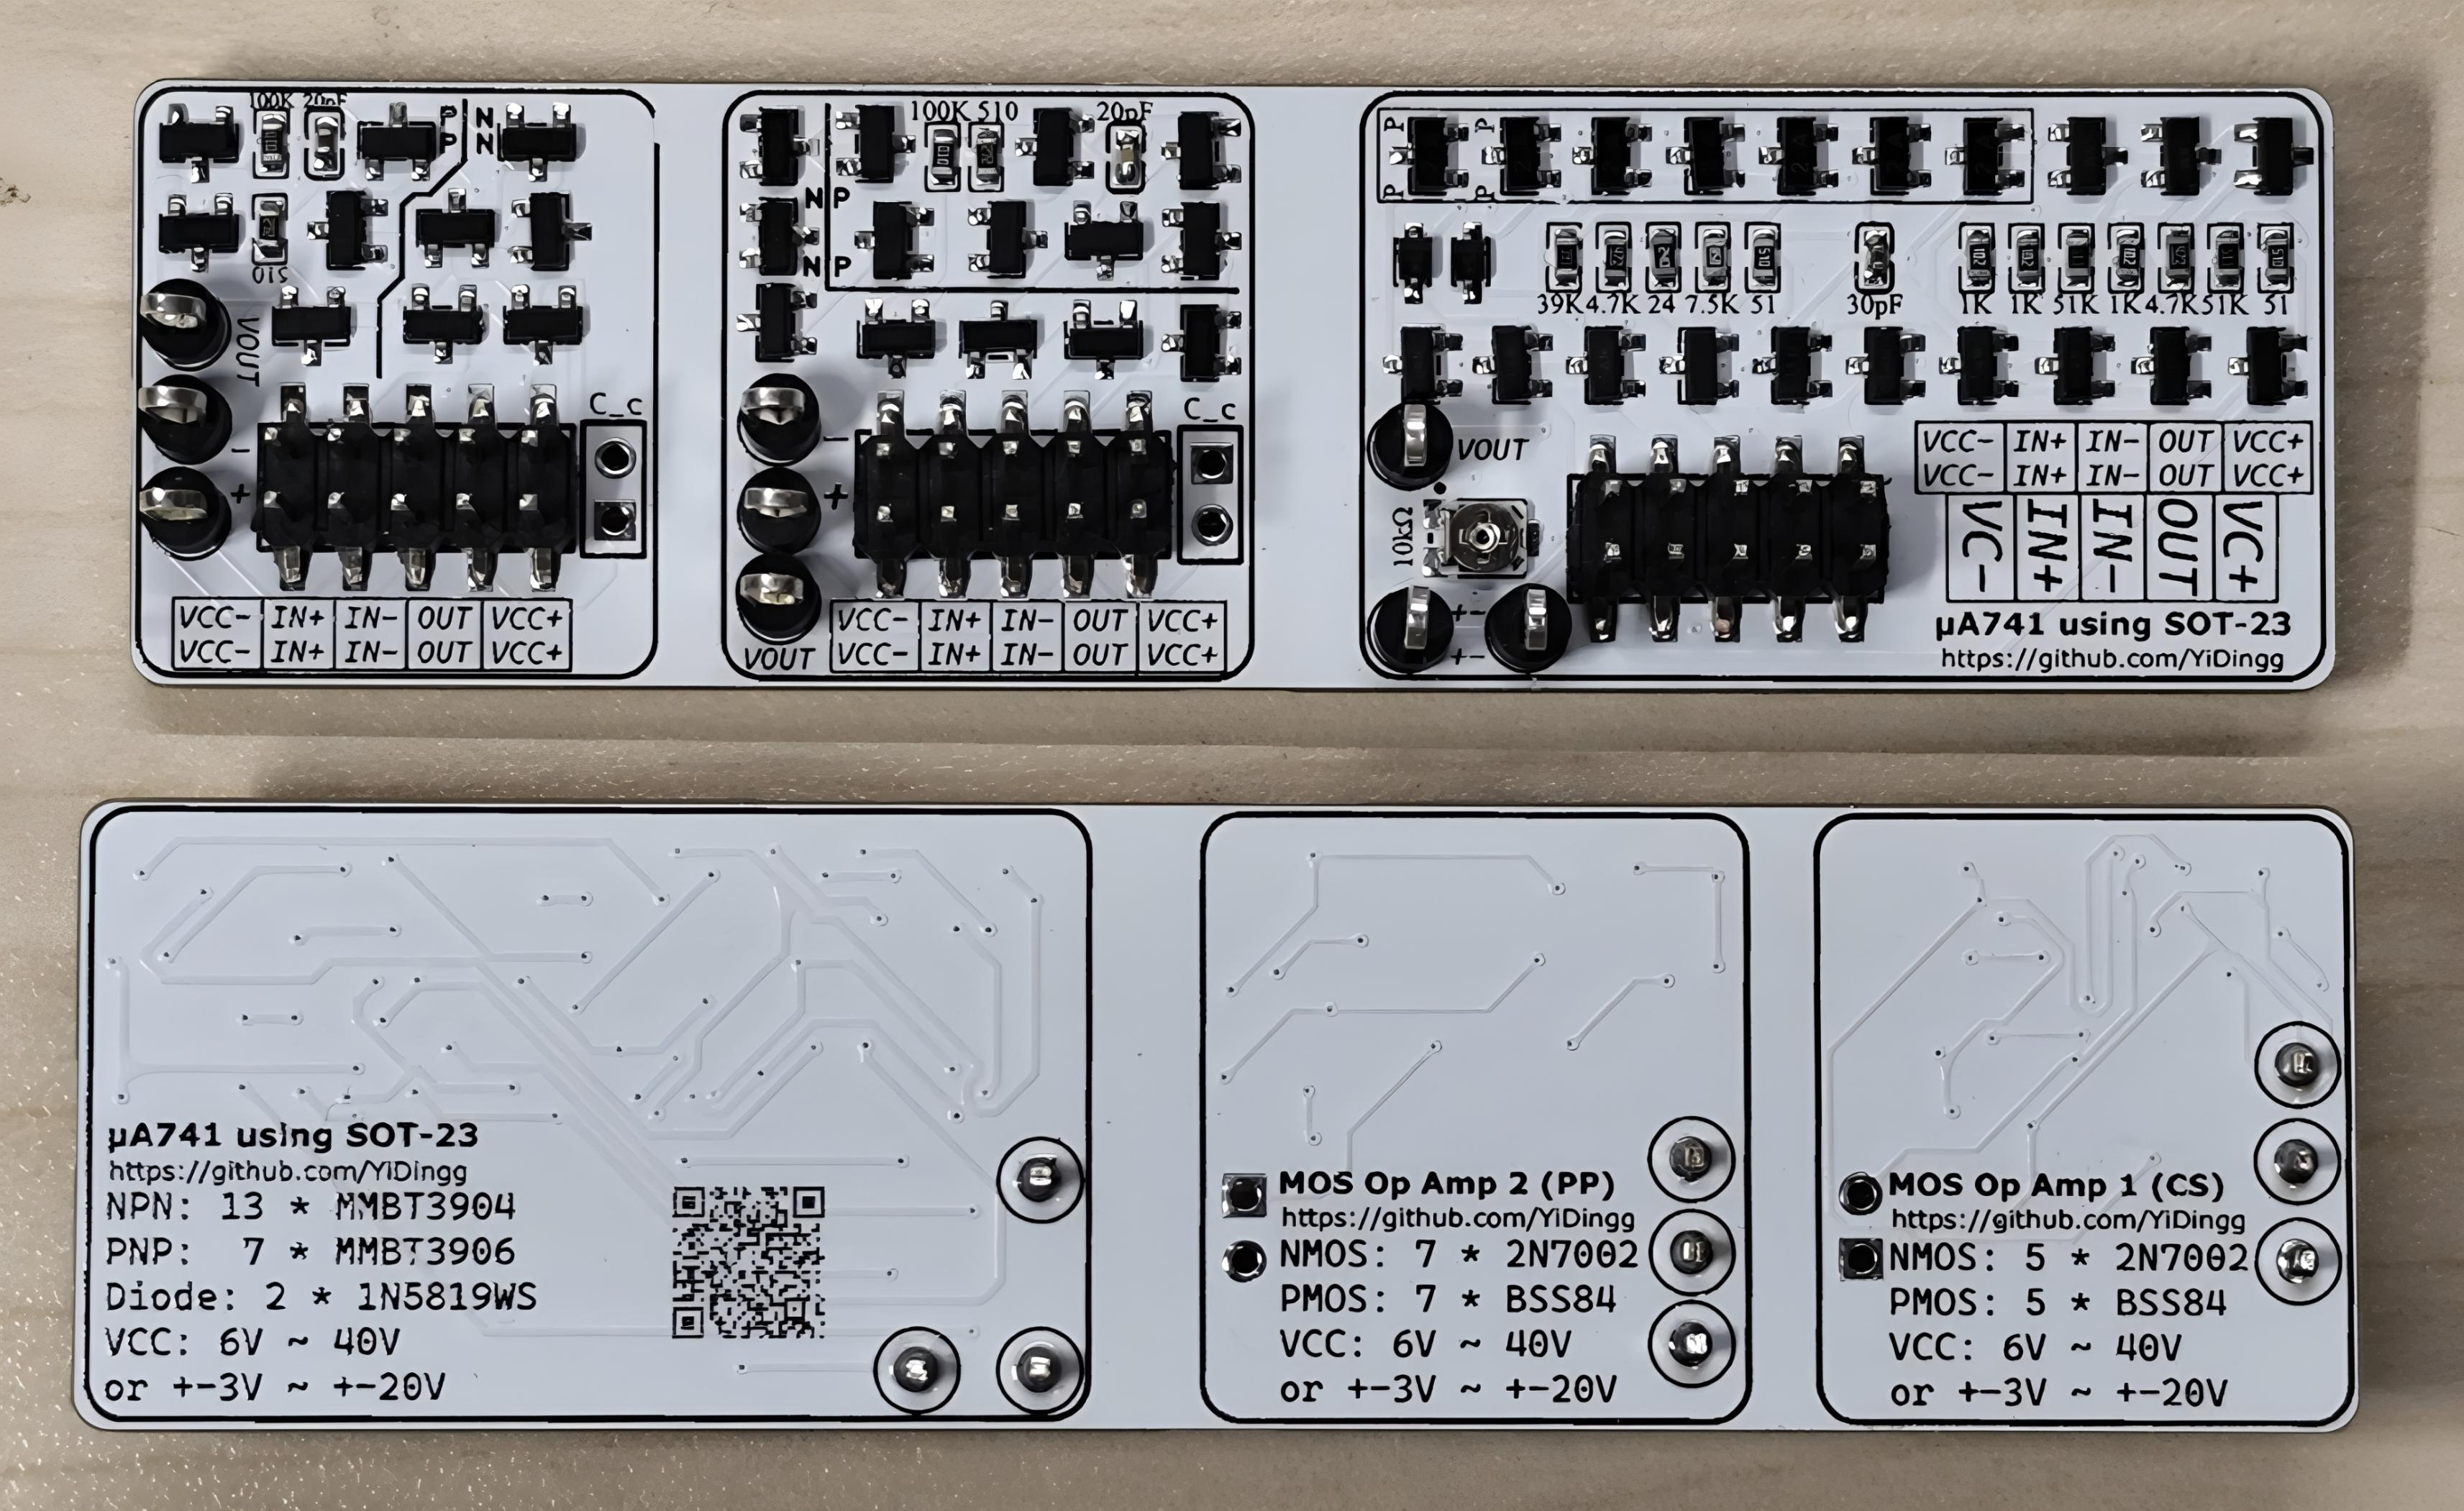
\includegraphics[width=\columnwidth]{LCE-06-07-运放设计/assets/demo.jpg}
    \caption{Demo preview of the self-designed discrete op amps}
\end{figure}

\begin{figure}[H]\centering
    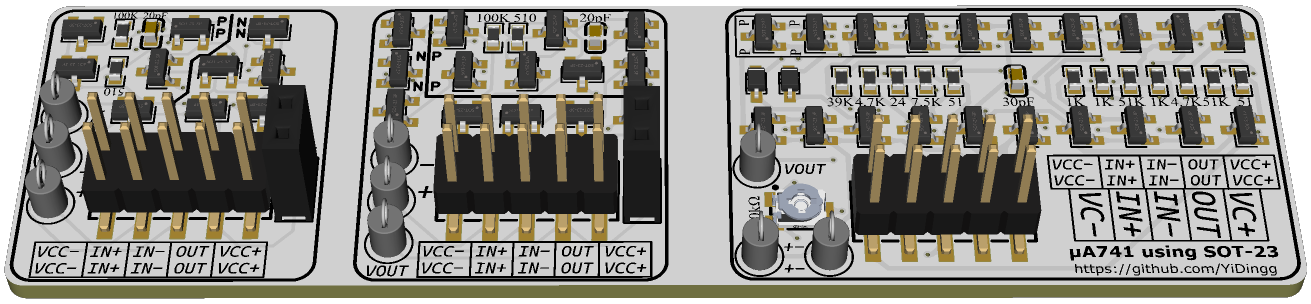
\includegraphics[width=\columnwidth]{LCE-06-07-运放设计/assets/3D.png}
    \caption{3D rendering graph of the tow CMOS op amps and the discrete uA741}
\end{figure}

\begin{figure}[H]\centering
    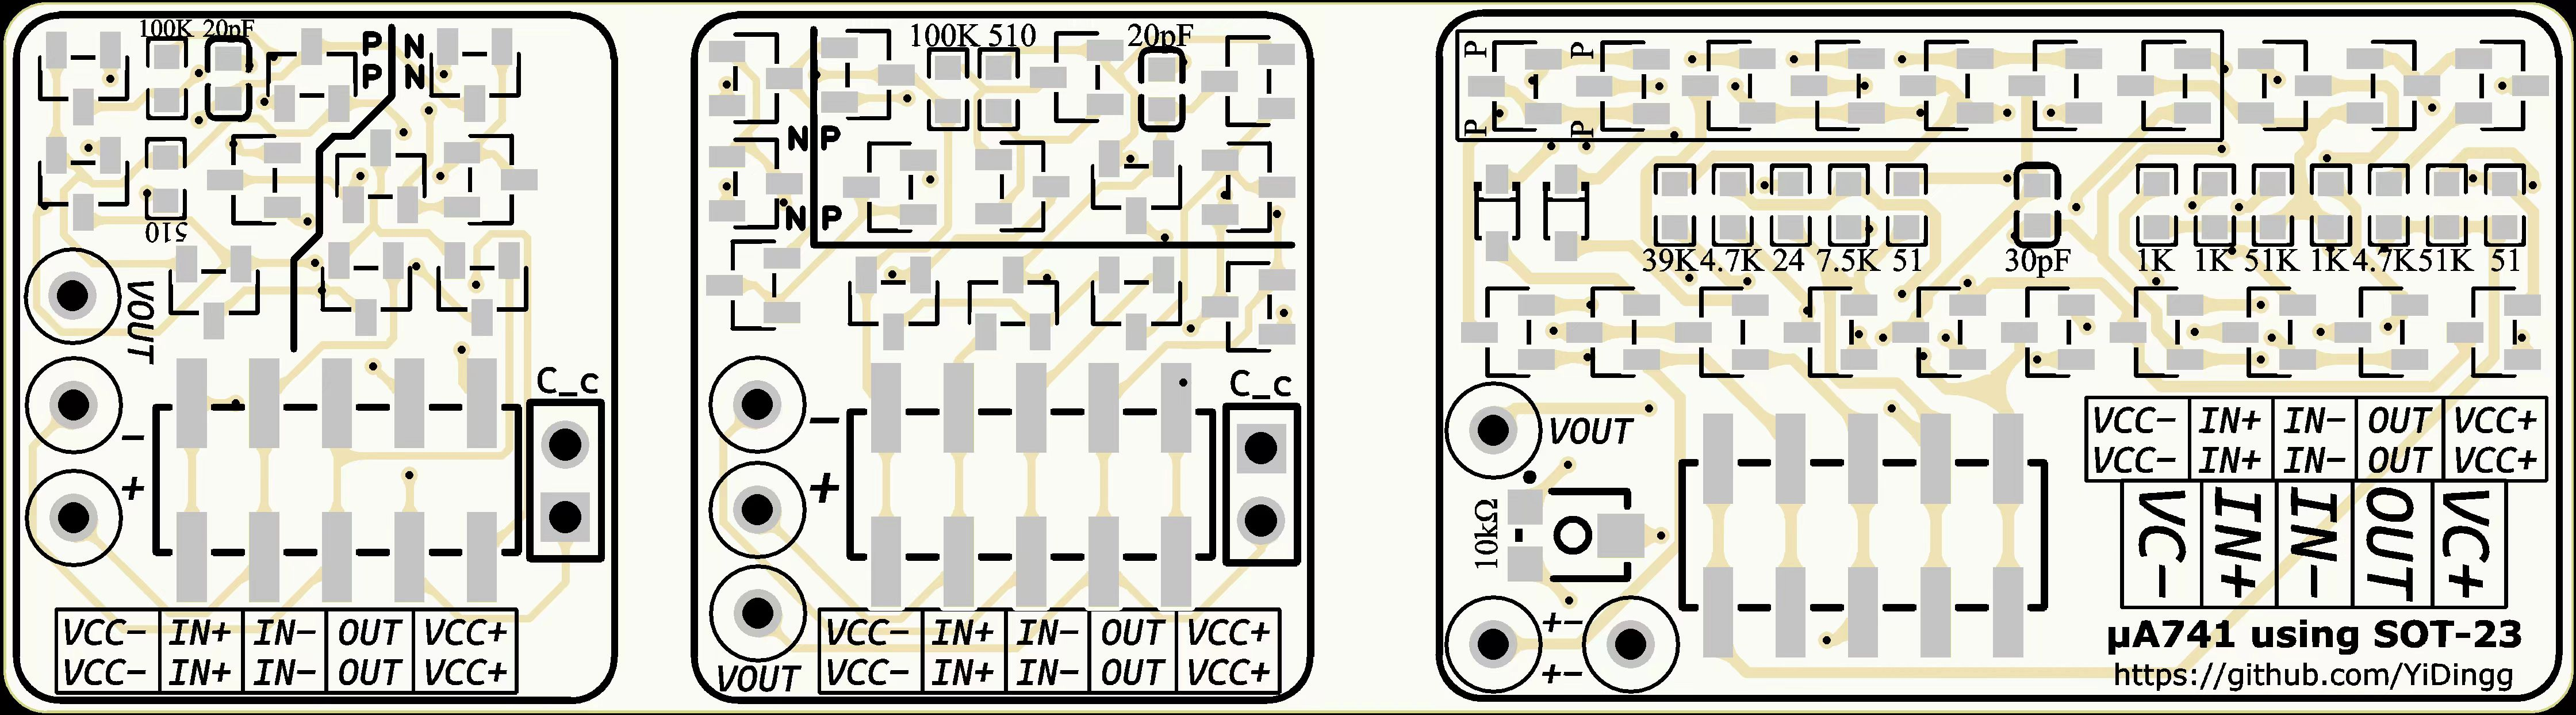
\includegraphics[width=\columnwidth]{LCE-06-07-运放设计/assets/2D top.jpeg}
    \caption{2D rendering graph of the tow CMOS op amps and the discrete uA741 (top view)}
\end{figure}

\begin{figure}[H]\centering
    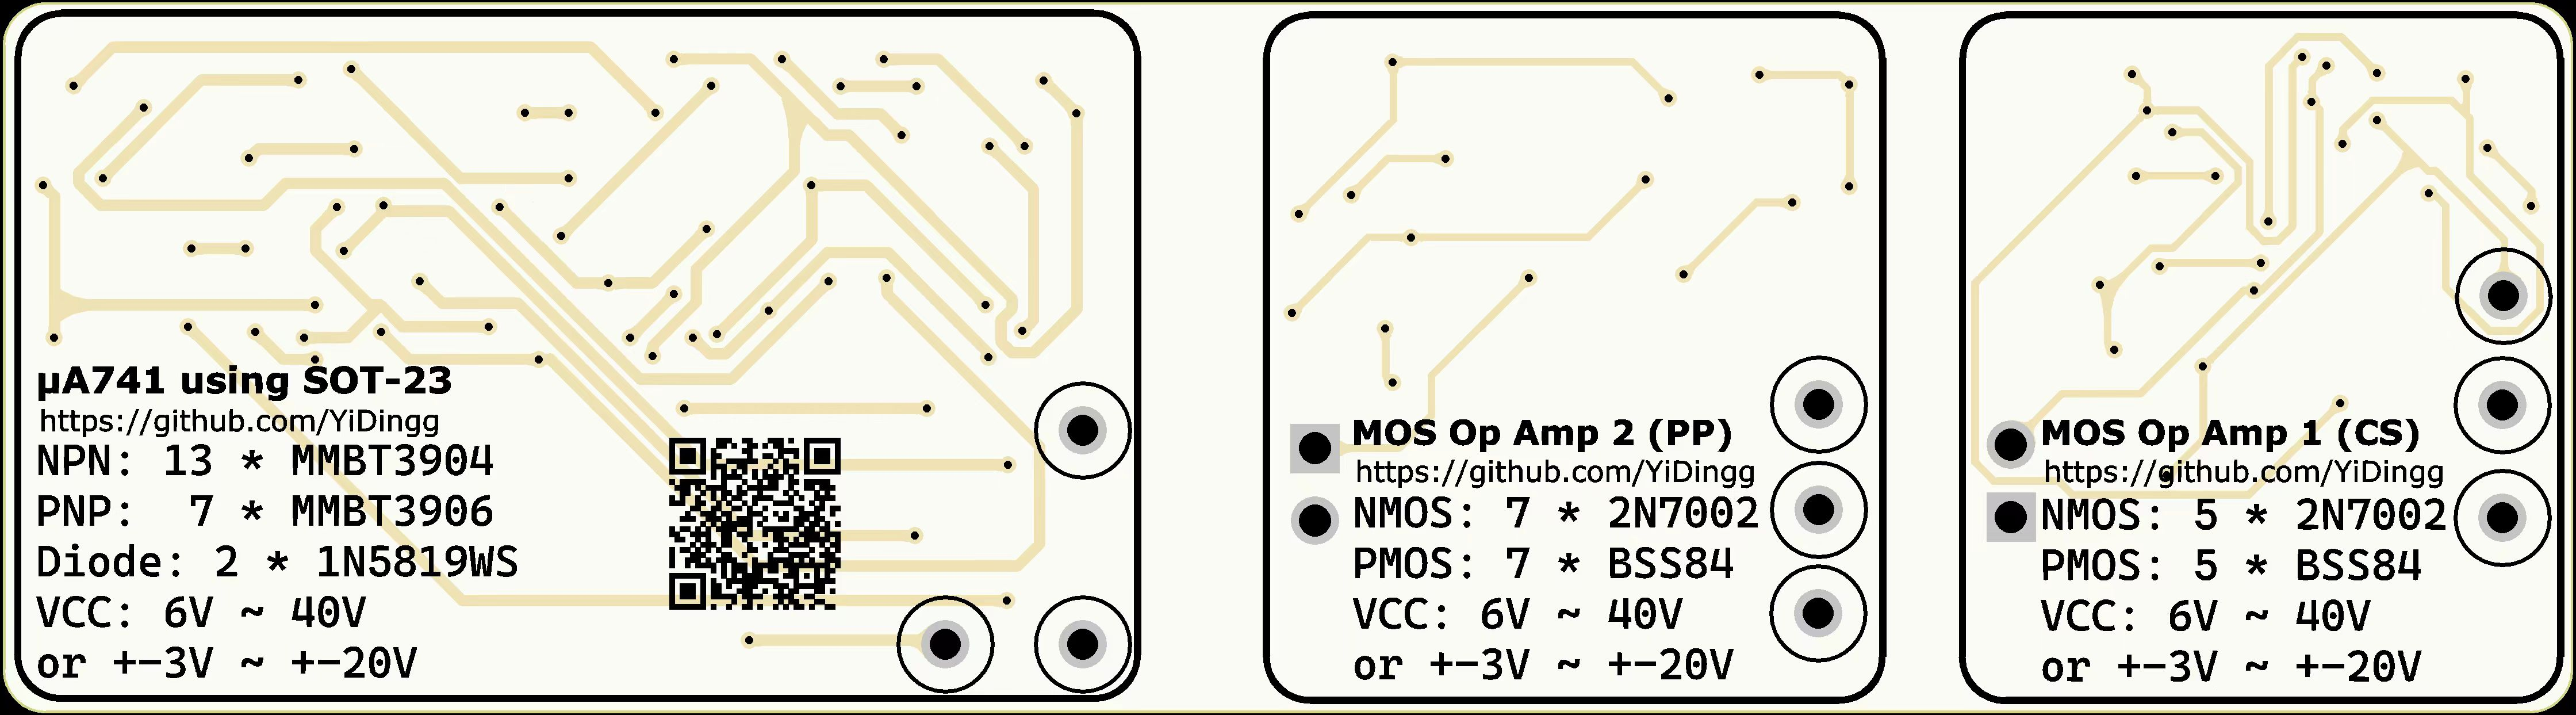
\includegraphics[width=\columnwidth]{LCE-06-07-运放设计/assets/2D bottom.jpeg}
    \caption{3D rendering graph of the tow CMOS op amps and the discrete uA741 (bottom view)}
\end{figure}


\subsection{CMOS Op Amp 1 (Common-Source Output Stage) }

\begin{figure}[H]\centering
    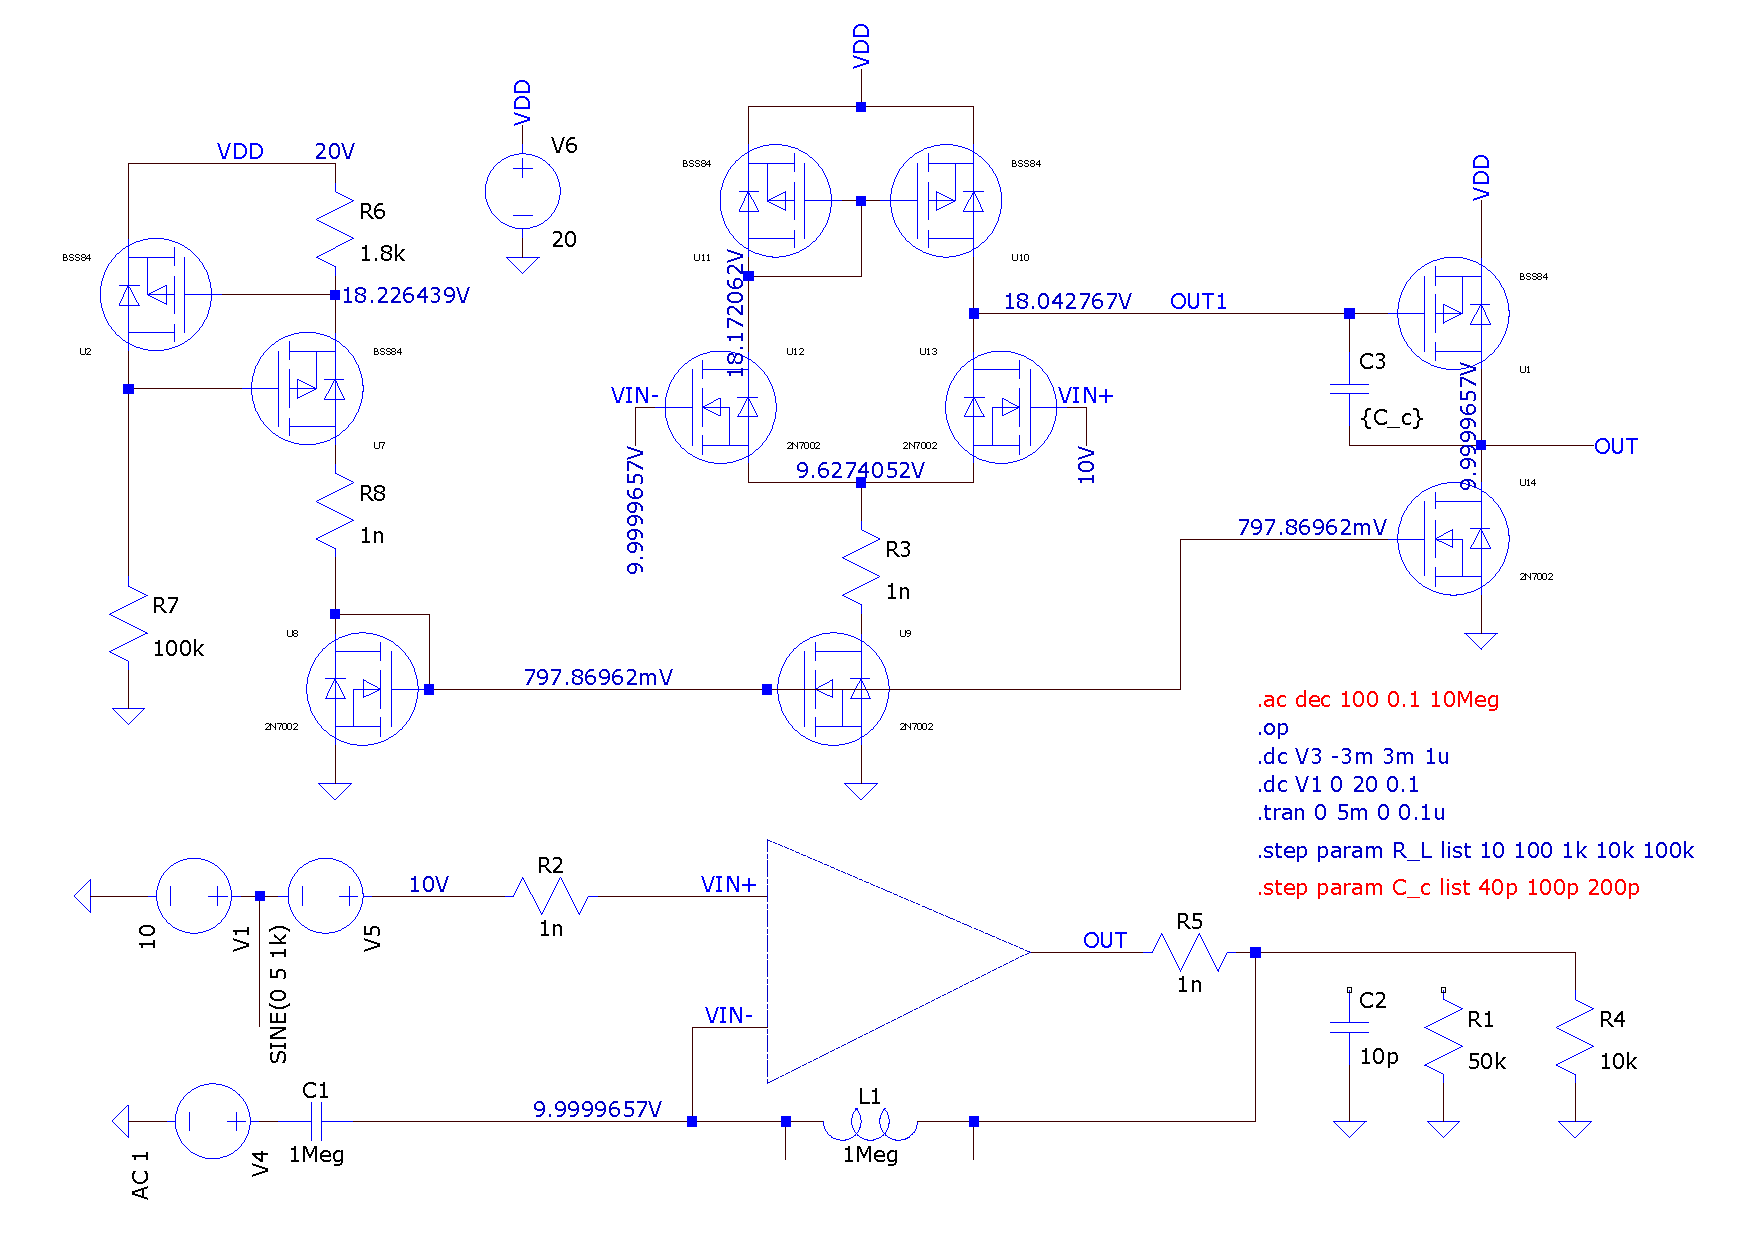
\includegraphics[width=0.91\columnwidth]{assets/op amp 1/CMOS op amp 1 (CS).pdf}
    \caption{Circuit schematic of CMOS Op Amp 1 (common-source output stage)}
    \label{fig: CMOS Op Amp 1}
\end{figure}

\begin{figure}[H]\centering
    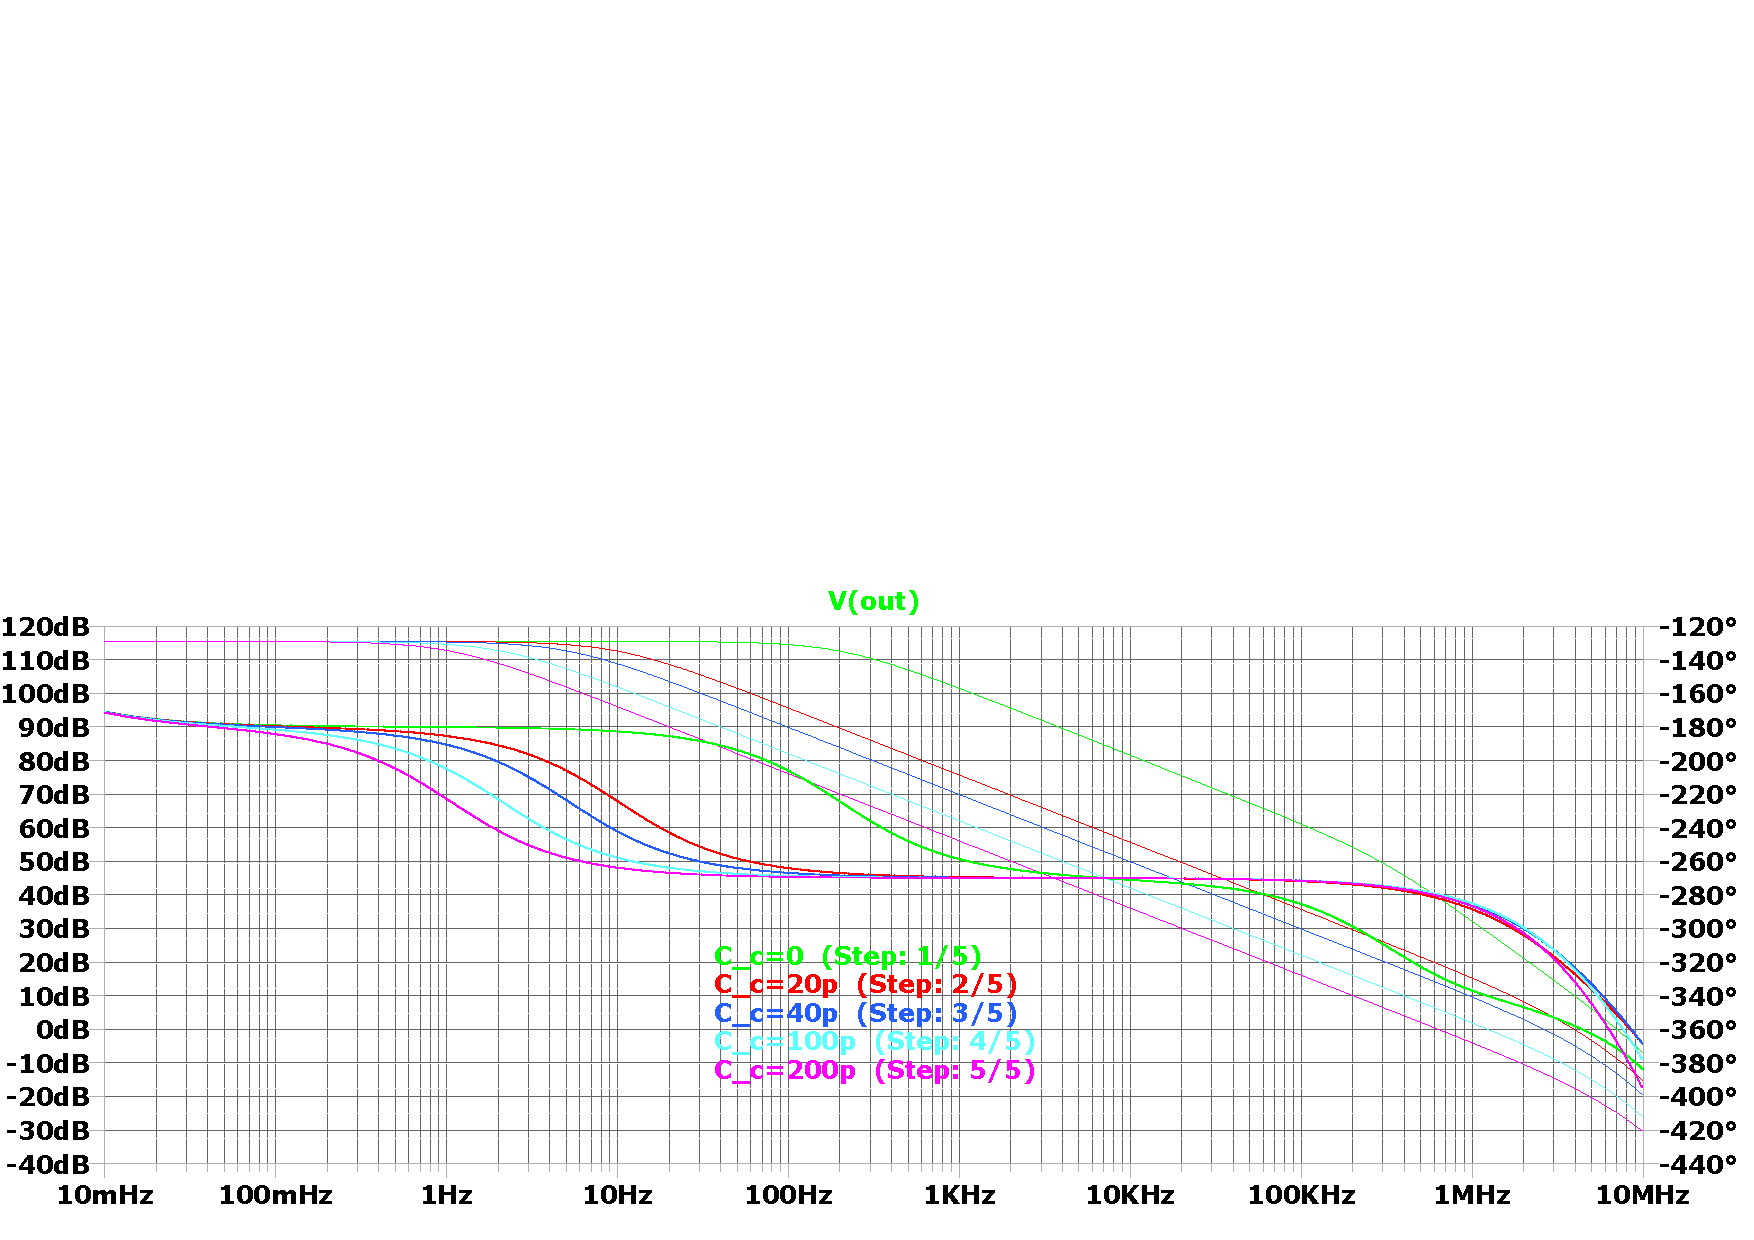
\includegraphics[width=0.91\columnwidth]{assets/op amp 1/gain of CMOS op amp 1 copy.pdf}
    \caption{Simulated frequency response of the CMOS op amp 1 (common-source output)}
\end{figure}

\subsection{CMOS Op Amp 2 (Improved Push-Pull Output Stage) }

\begin{figure}[H]\centering
    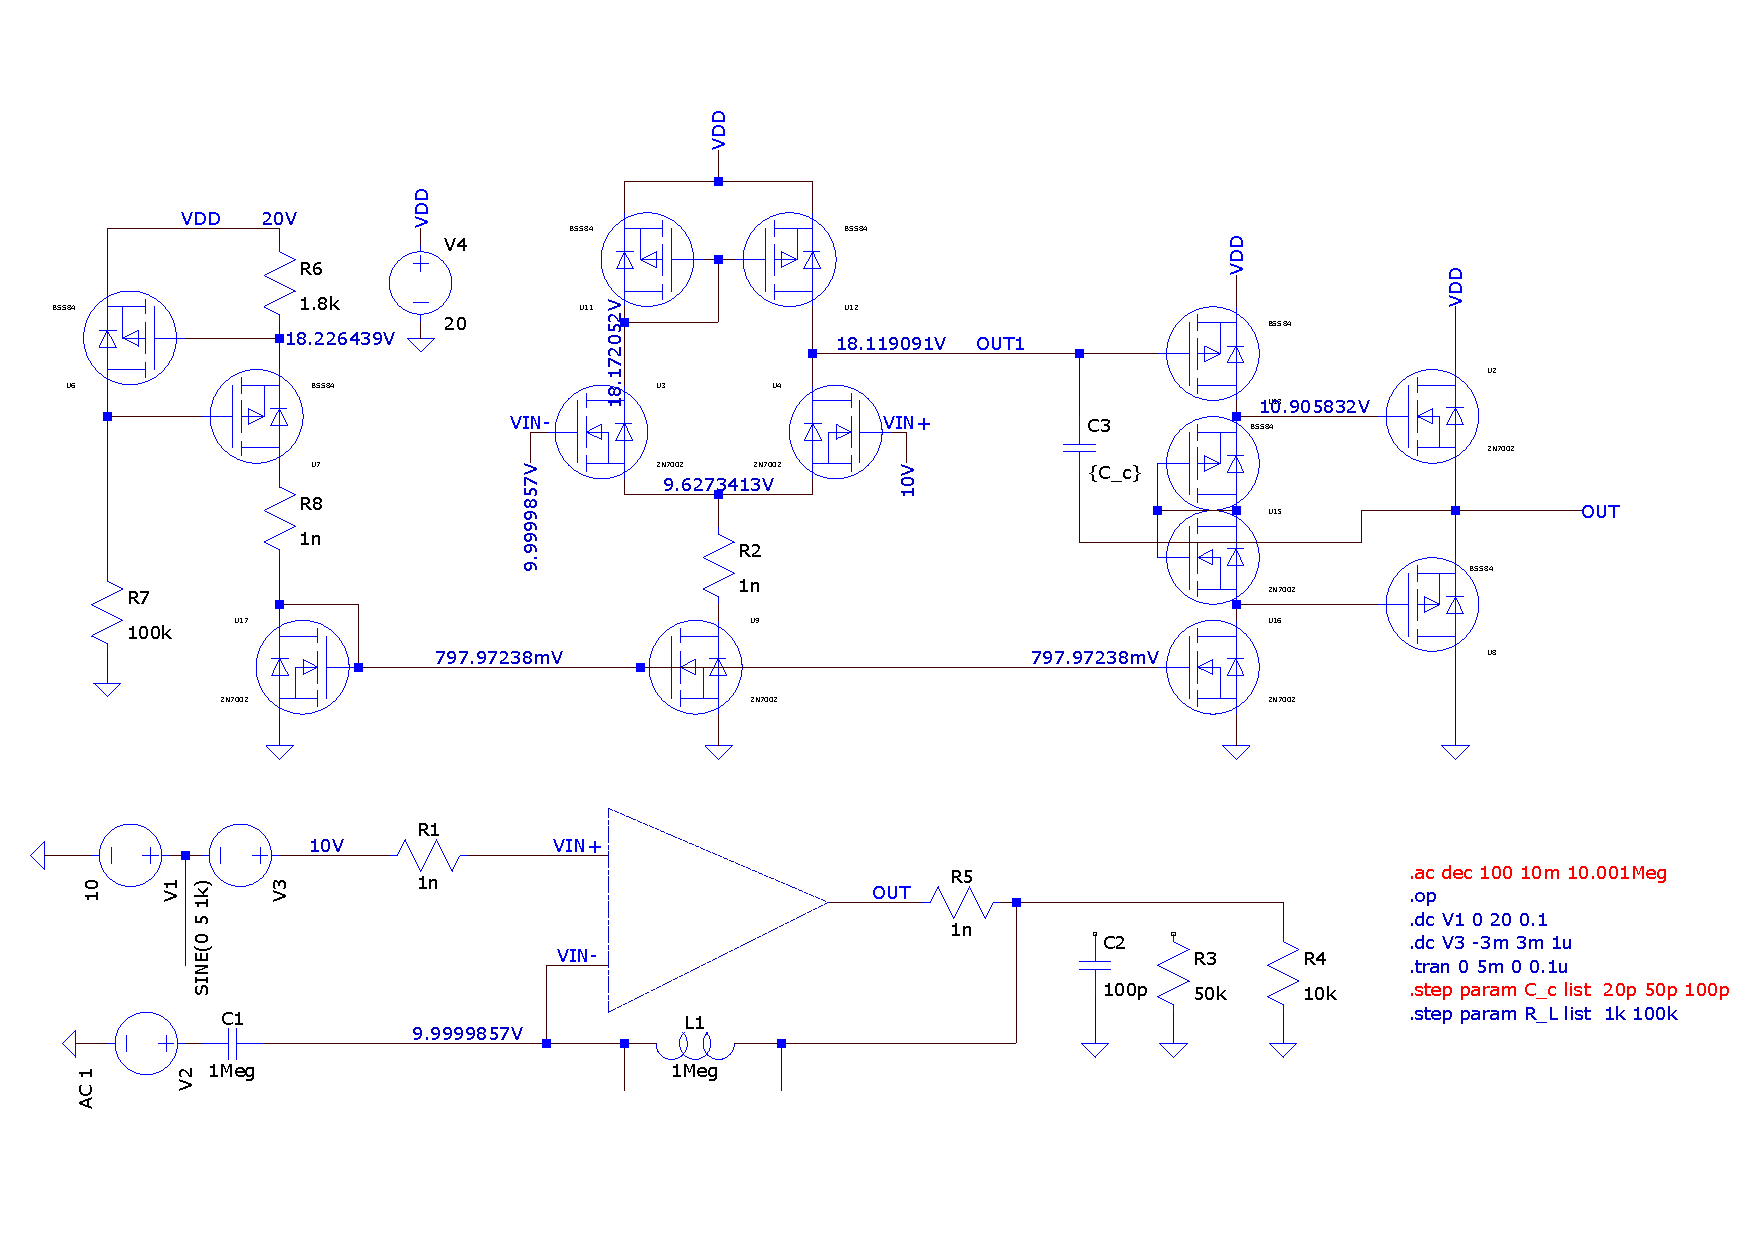
\includegraphics[width=0.91\columnwidth]{assets/op amp 2/CMOS op amp 2 (PP).pdf}
    \caption{Circuit schematic of CMOS Op Amp 2 (improved push-pull output stage)}
    \label{fig: CMOS Op Amp 2}
\end{figure}

\begin{figure}[H]\centering
    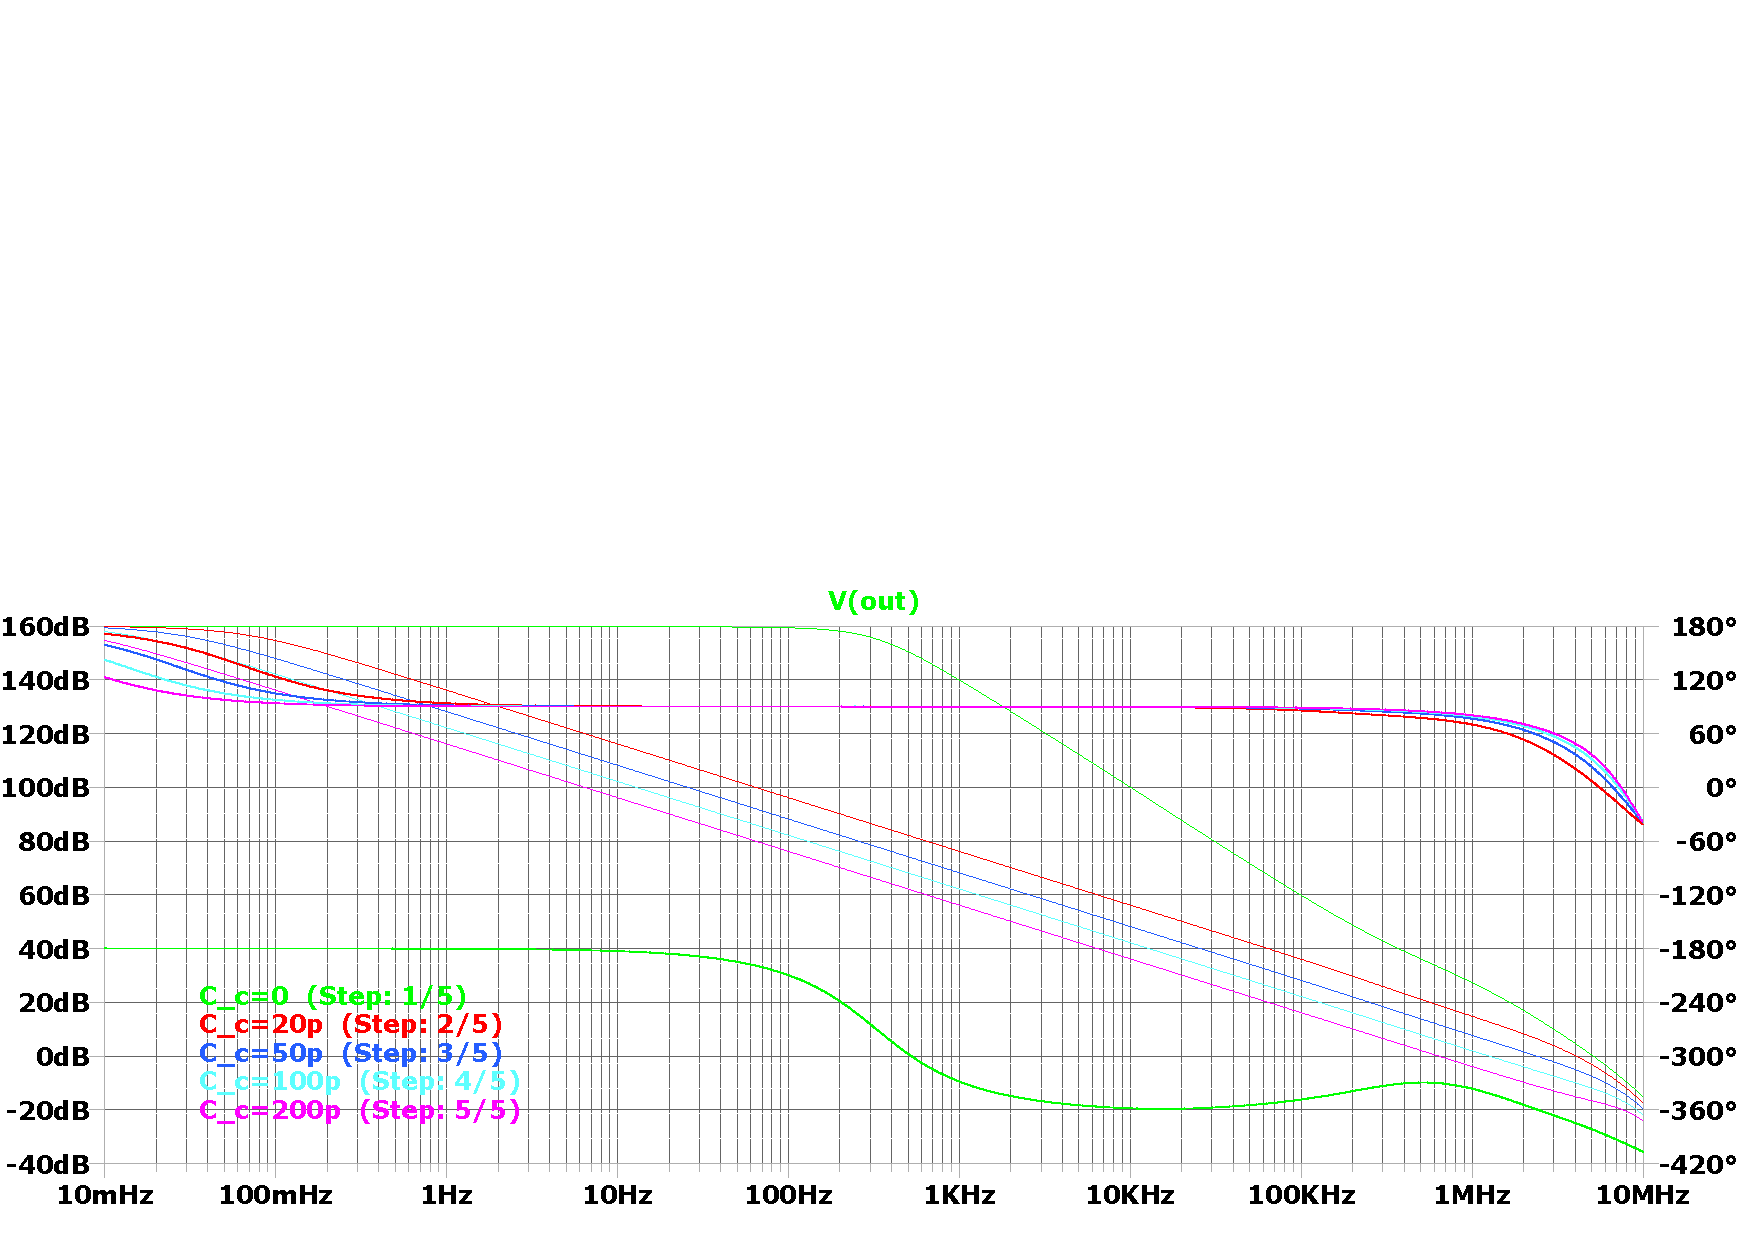
\includegraphics[width=0.91\columnwidth]{assets/op amp 2/gain of CMOS op amp 2 copy.pdf}
    \caption{Simulated frequency response of the CMOS op amp 2 (improved push-pull output)}
    \label{gain of CMOS op amp 2}
\end{figure}

\subsection{μA741 using Discrete BJTs}
\vspace*{-2mm}
\subsubsection{Circuit Schematic and Block Diagram}
\vspace*{-6mm}
\begin{figure}[H]\centering
    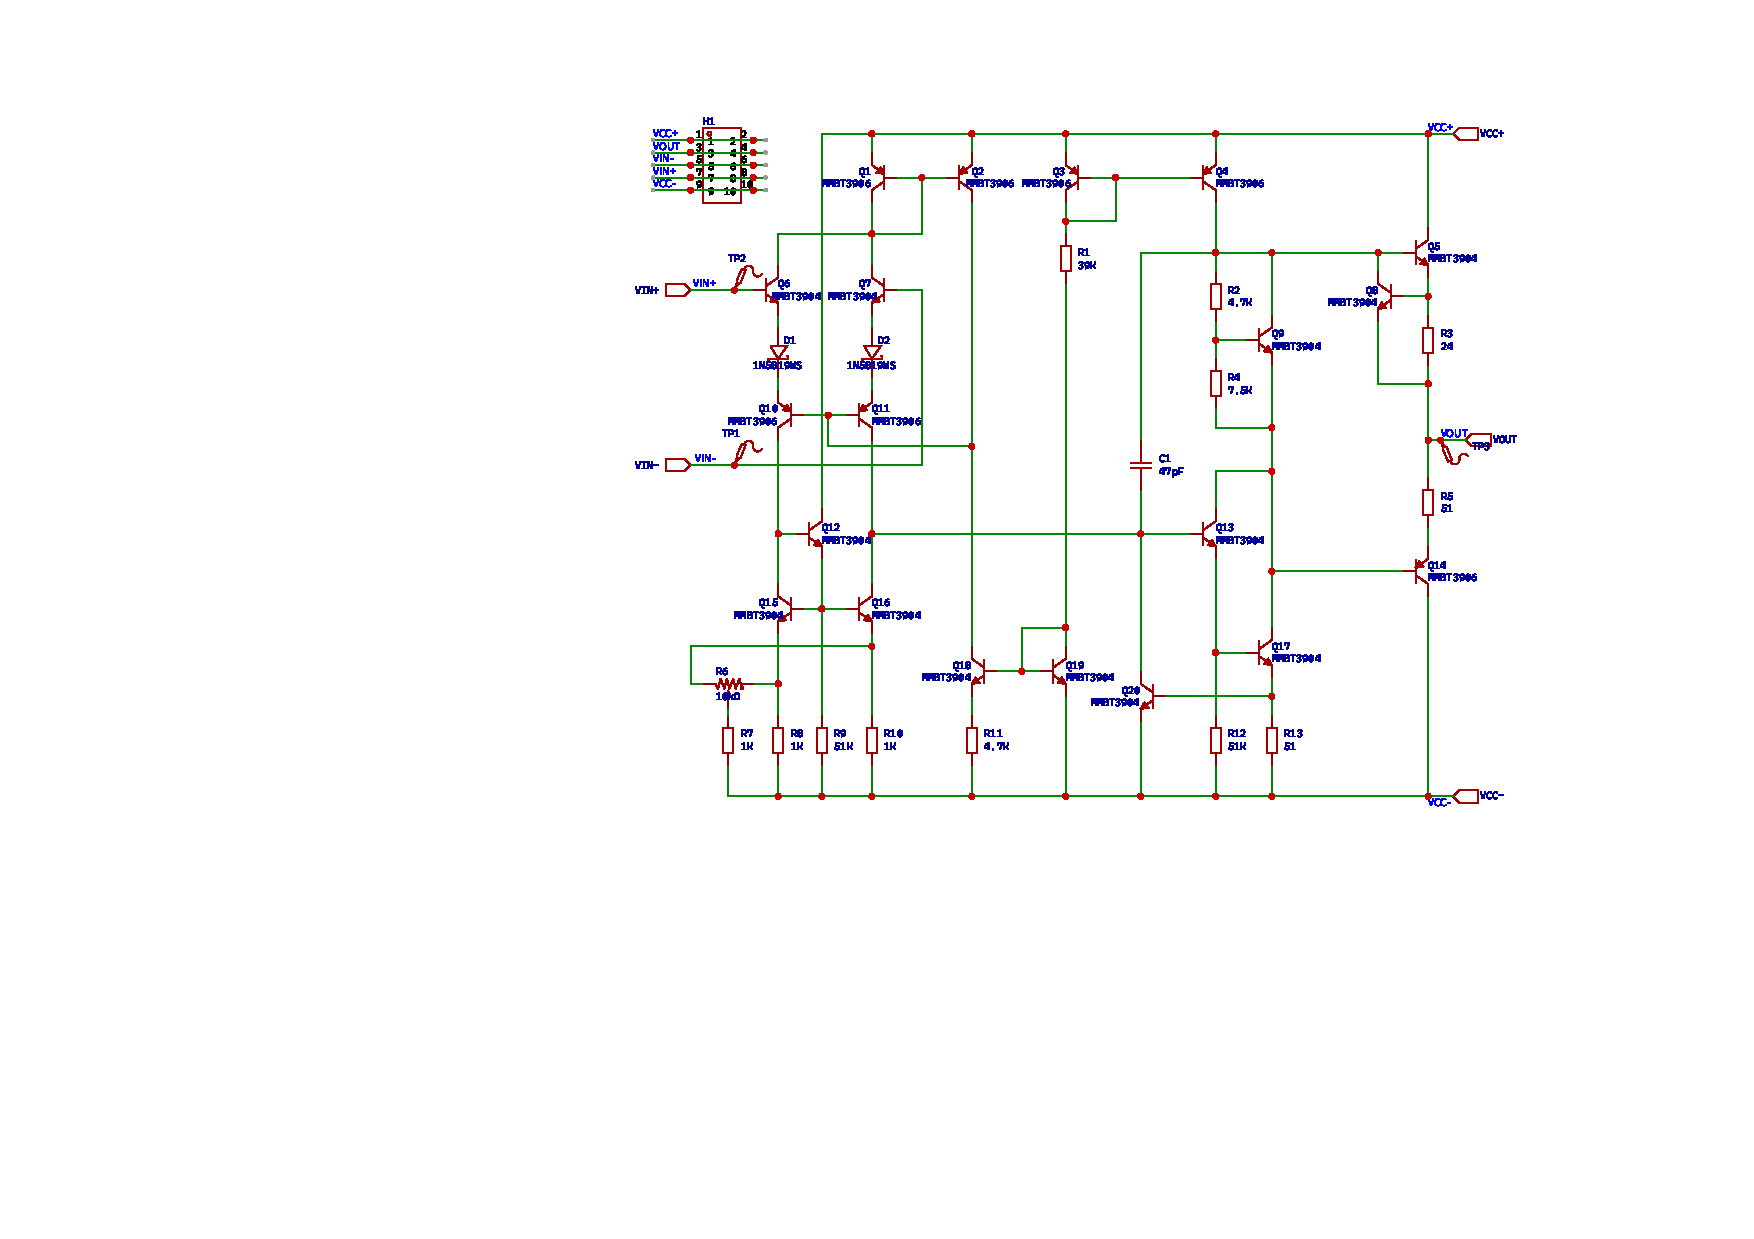
\includegraphics[width=0.79\columnwidth]{LCE-06-07-运放设计/assets/uA741/SCH_Schematic1_1-P1_2025-05-15.pdf}
    \caption{Circuit schematic of the discrete μA741}
\end{figure}
\begin{figure}[H]\centering
    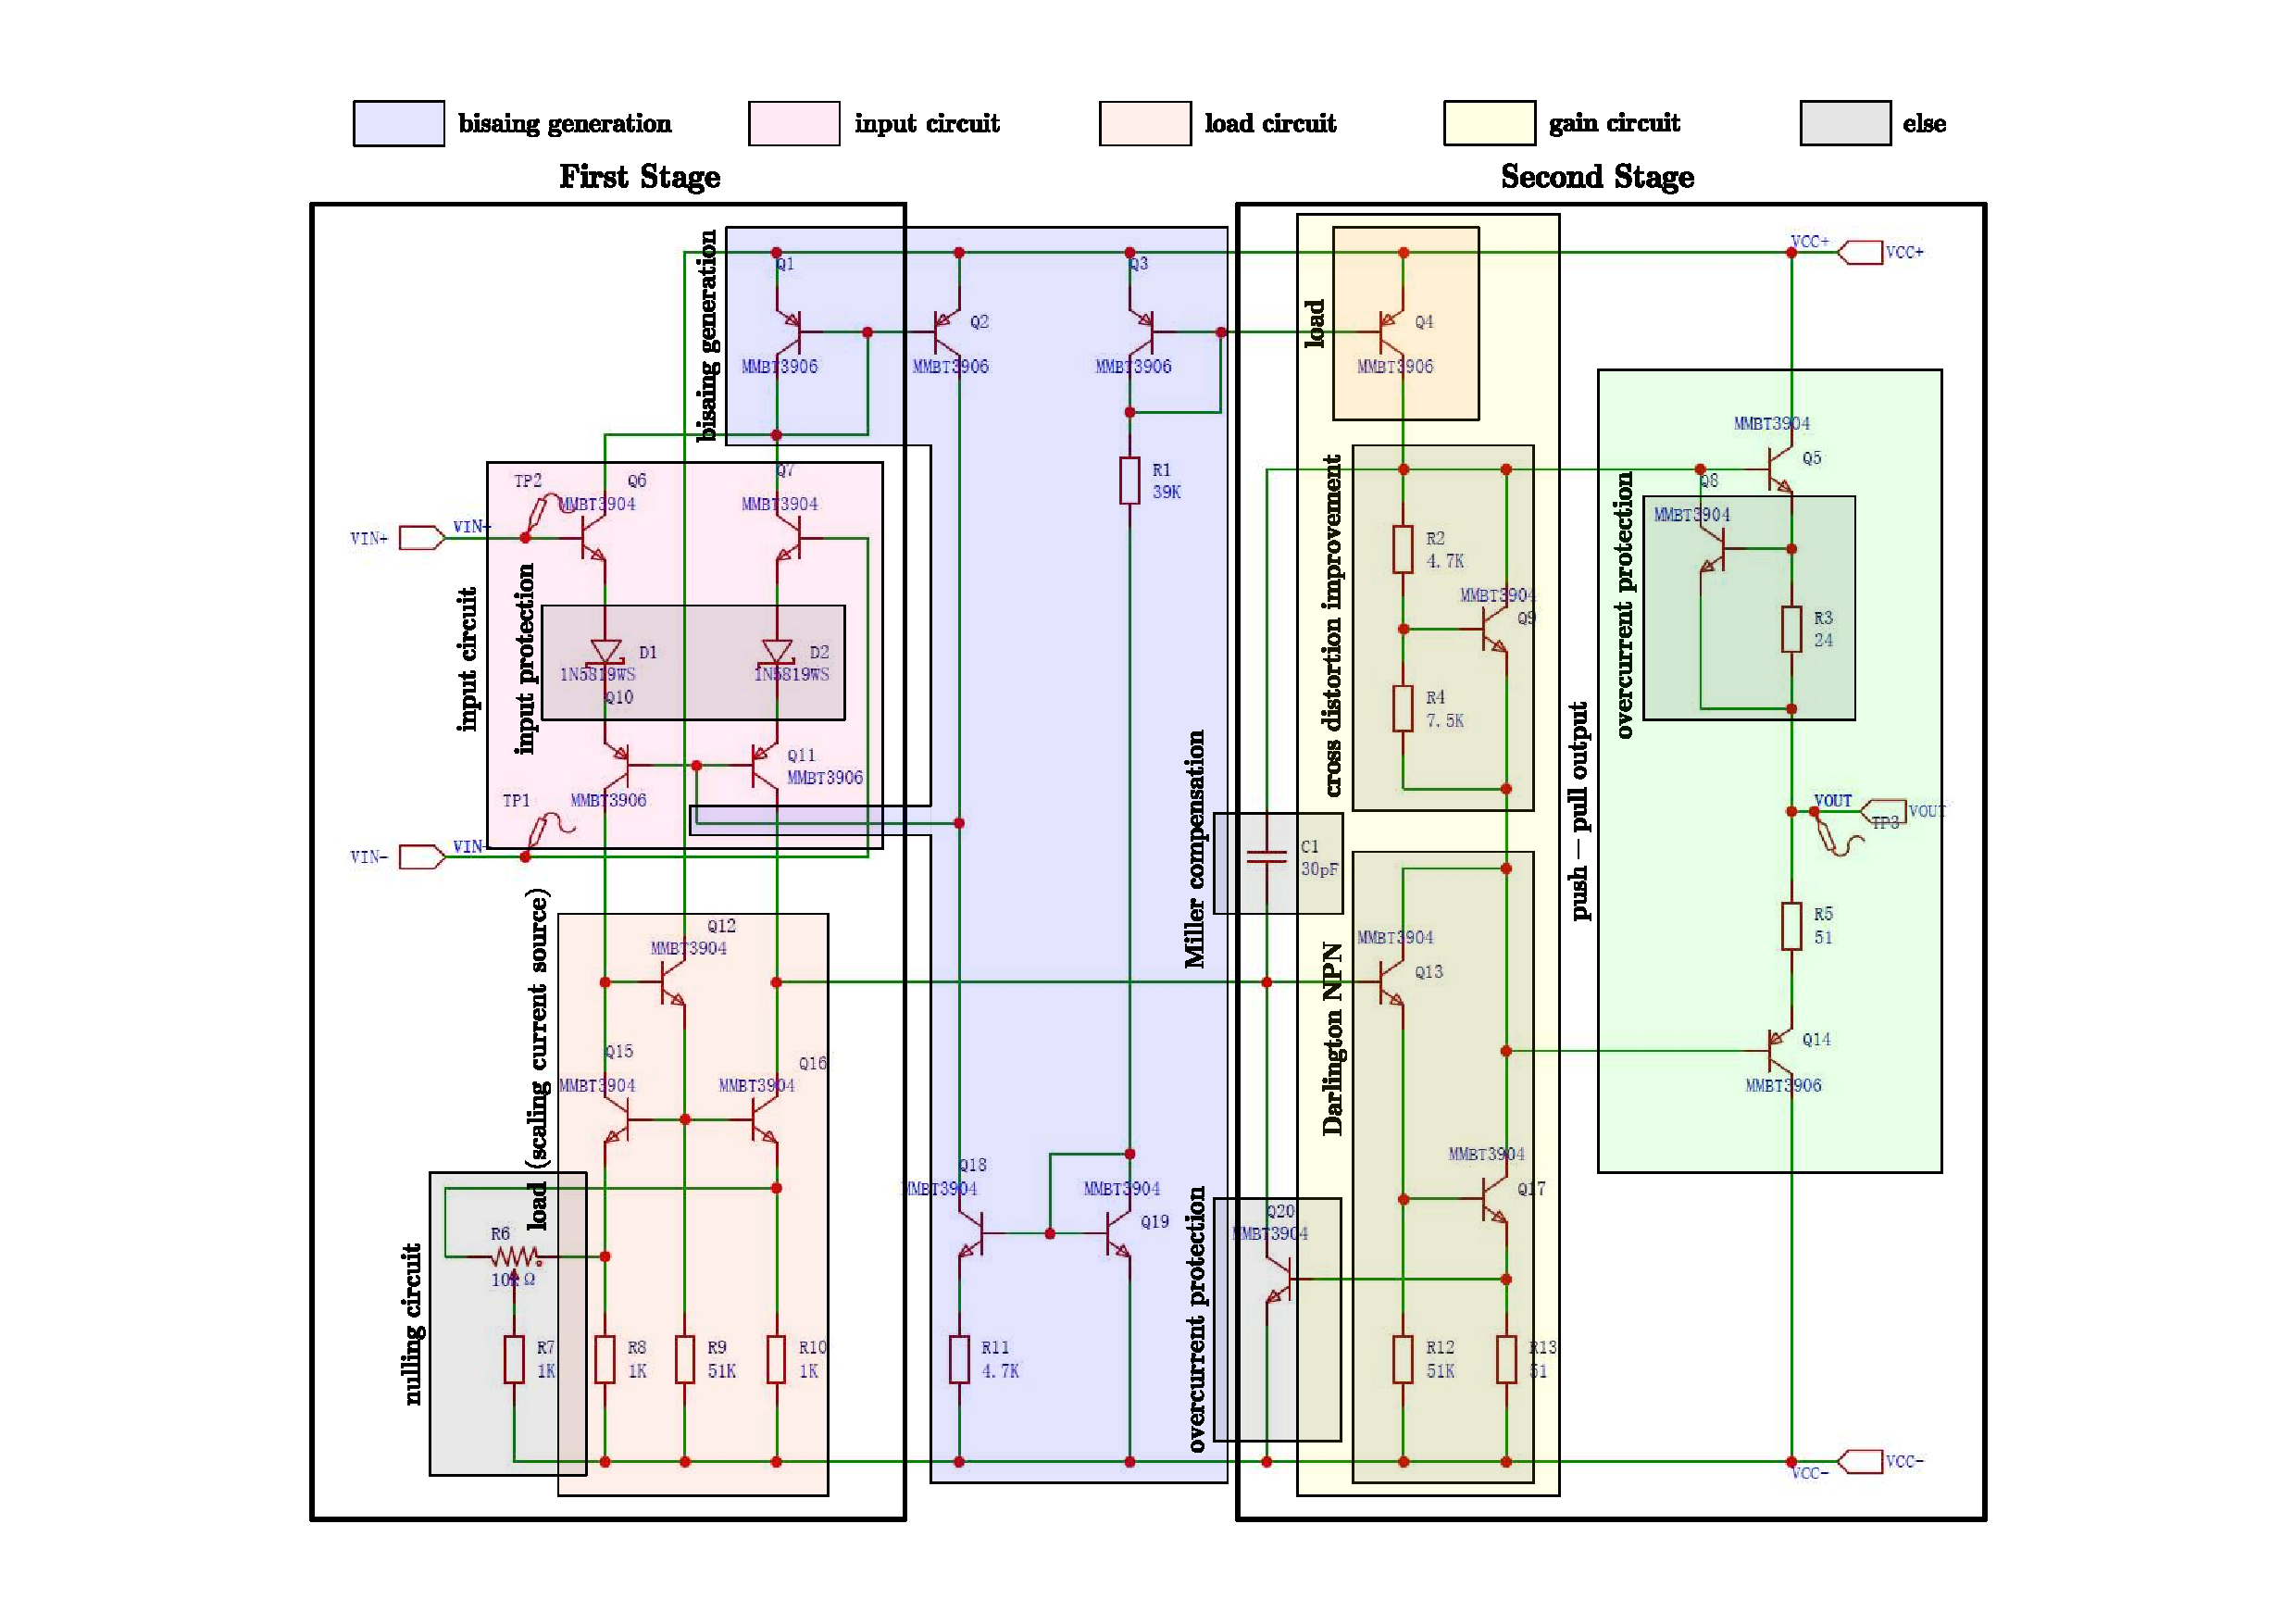
\includegraphics[width=0.79\columnwidth]{assets/uA741/uA741 block.pdf}
    \caption{Block diagram analysis of the discrete μA741}
\end{figure}

\subsubsection{Biasing Analysis}



\begin{center}
\noindent\begin{minipage}{0.49\columnwidth}
    \hspace*{1em} Q3, R1 and Q19 together constitute the fundamental biasing of the op amp, generating a current of $I_0 = \frac{V_{CC} - 1.4 \ \mathrm{V}}{r_{out1}} = \frac{V_{CC} - 1.4 \ \mathrm{V}}{39 \ \mathrm{k}\Omega}$. Note that Q18 and R11 form microampere current source, the collector current of $Q_{18}$ satisfies the equation:
    \begin{equation}
        I_1 \approx \frac{V_T}{R_{11}} \ln \left(\frac{I_{REF}}{I_1}\right) \Longleftrightarrow I_{REF} = I_1 \cdot e^{\frac{R_{11}I_1}{V_T}}
    \end{equation}
    \hspace*{1em} Since $I_{REF}$ changes in an exponential relationship as $I_1$ varies, the resulting $I_1$ becomes relatively constant. Assuming $V_T = 26\ \mathrm{mV}$ and sketch the curve $I_1 = I_1 (I_{REF})$ as shown in the figure on the right.

    \hspace*{1em} For the power supply varying from 10 V to 40 V, $I_1$ is within the range of $15 \ \mathrm{uA} \sim 22 \ \mathrm{uA}$. We assume $I_1 = 20 \ \mathrm{uA}$ in the following analysis.
\end{minipage}\hfill\begin{minipage}{0.49\columnwidth}
\begin{figure}[H]\centering
    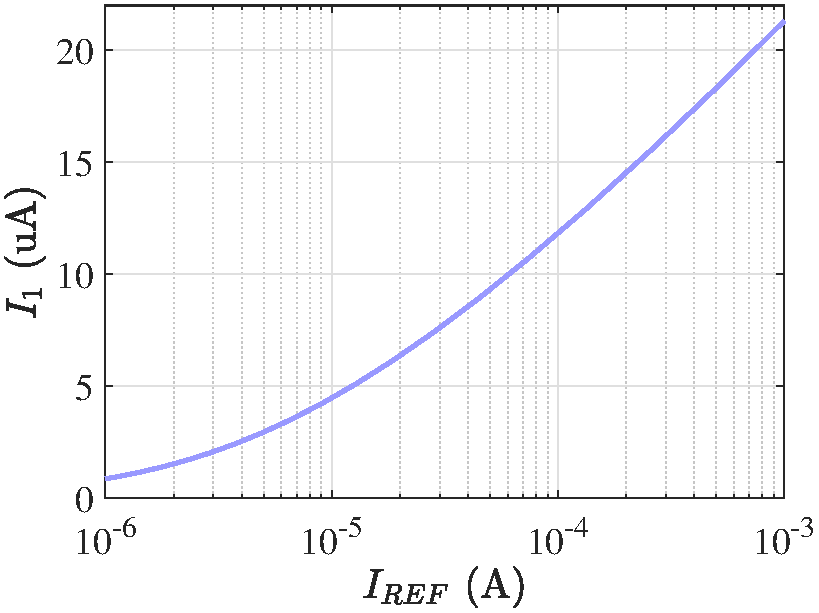
\includegraphics[width=\columnwidth]{LCE-06-07-运放设计/assets/uA741/I_1.pdf}
    \caption{Variation of $I_1$ as a function of $I_{REF} = I_0$}
\end{figure}
\end{minipage}\end{center}

Noticing that the combination of Q6 and Q10 (CC-CB structure) can be viewed as a high-performance PNP transistor. Therefore, based on $I_1$ (the current of Q18), Q1, Q2 and the input block form a Wilson current source, copying $I_1$ to the input stage. On the other hand, Q4 copies the current $I_1$ from the base of Q3, defining the operation point of Q4 and Q13 + Q17 (a Darlington NPN pair).
\begin{figure}[H]\centering
    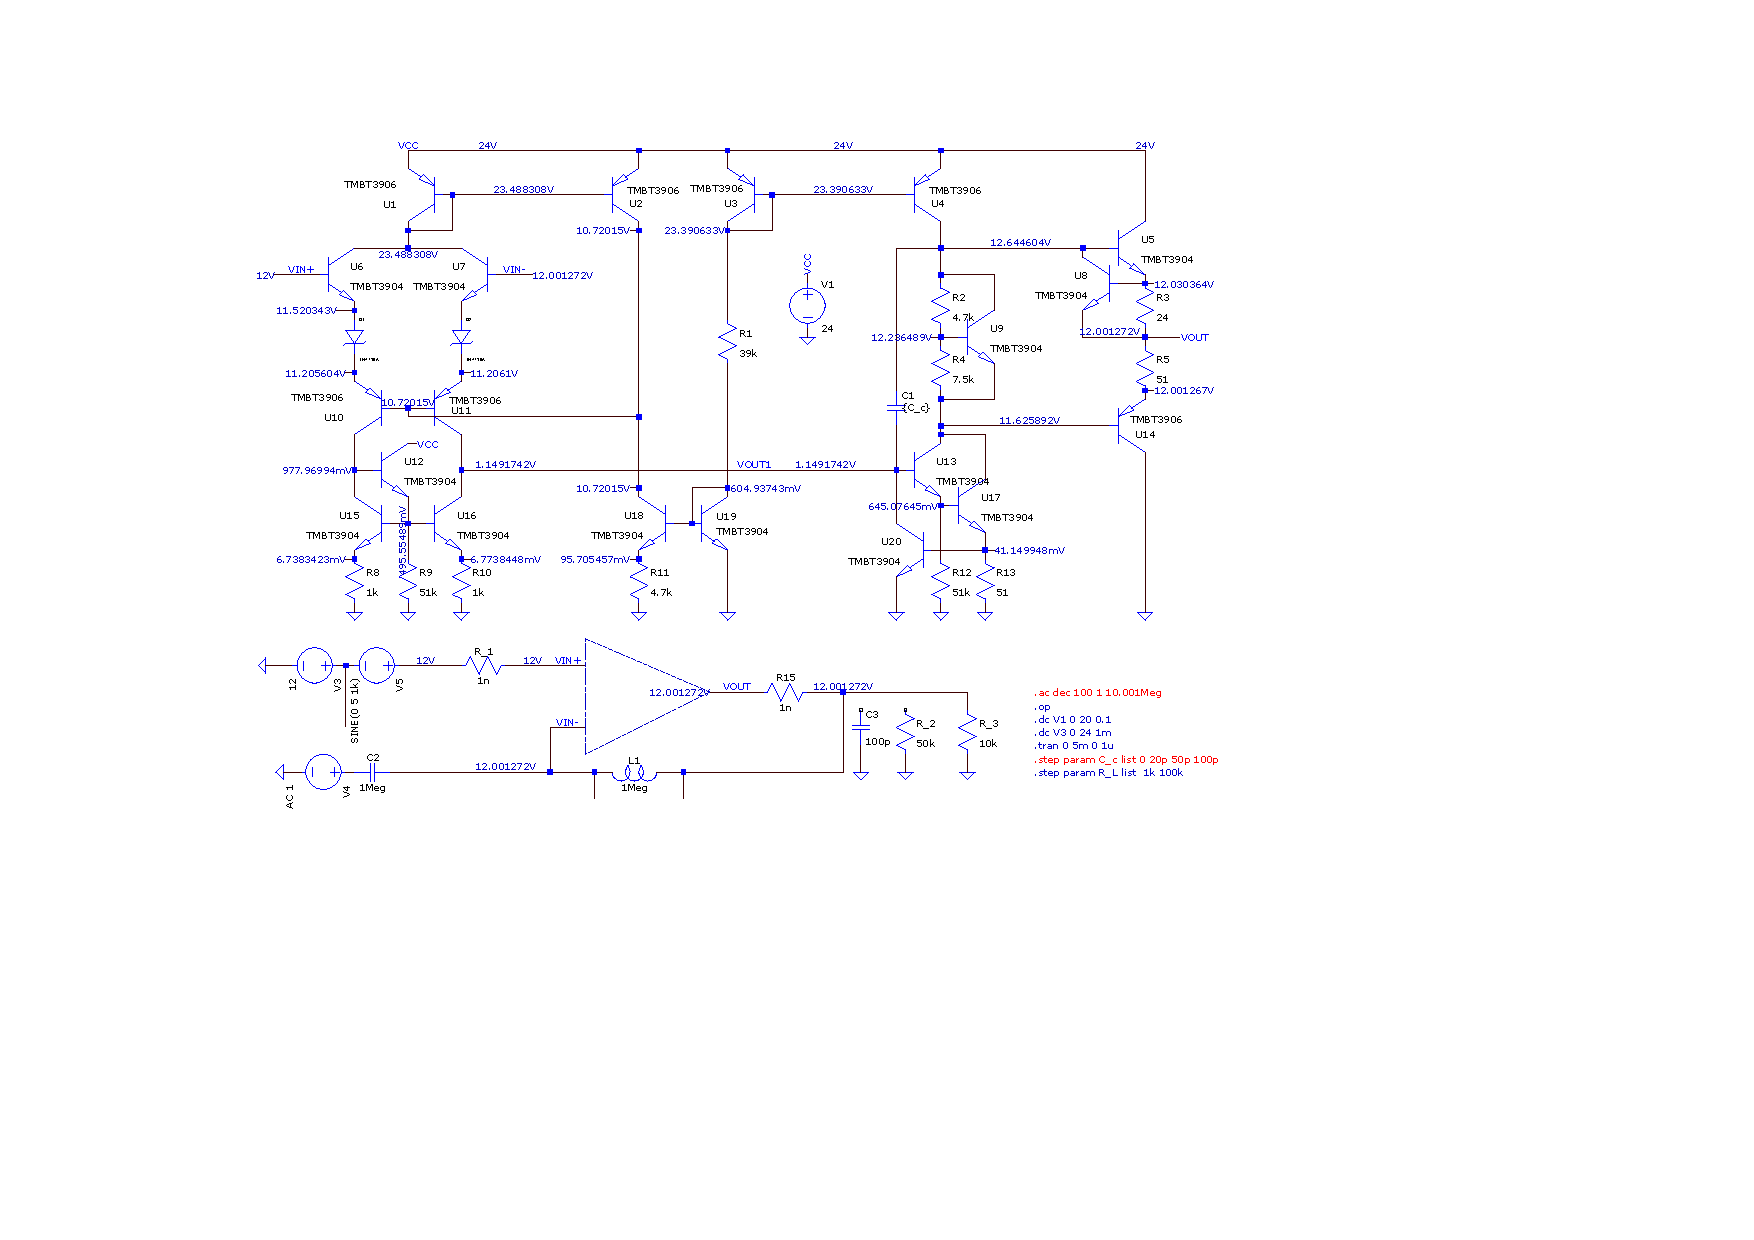
\includegraphics[width=0.91\columnwidth]{LCE-06-07-运放设计/assets/uA741/uA741 LTspice.pdf}
    \caption{LTspice simulation of the discrete μA741}
    \label{LTspice uA741}
\end{figure}
\noindent 
Setting $V_{CC} = 24 \ \mathrm{V},\ V_{IN+} = V_{IN-} = 12 \ \mathrm{V}$ and config the op amp as a unit buffer, the simulation gives that:
\begin{gather}
    |I_{C,Q3}| = I_{C,Q19} = 0.58 \ \mathrm{mA},\quad 
    |I_{C,Q2}| = I_{C,Q18} = 20.21 \ \mathrm{uA},\ 
    |I_{C,Q1}| = 13.31 \ \mathrm{uA},\ 
    |I_{C,Q4}| = 0.82 \ \mathrm{mA}
\end{gather}
which verified the conclusions above.



\subsubsection{Small-Signal Analysis}

The Wilson current mirror, as the active load of the input stage, exhibits an output resistance of $r_{out1} \approx R_{coll}$, which can be approximated as:
\begin{align}
    r_{out1} &\approx R_{coll} 
    \\
    &= r_O \left[1 + \left(\frac{\beta}{r_{\pi} + R_B} + \frac{1}{r_O}\right)\cdot \left(R_E \parallel (r_{\pi} + R_B)\right)\right] 
    \\ 
    &\approx r_O + (1 + g_m r_O) (R_E \parallel r_{\pi})\quad {\color{gray} (R_B = 0)}
    \\ 
    &\approx r_O + (1 + g_m r_O)R_E \quad {\color{gray} (r_{\pi} = \frac{\beta V_T}{I_C} \gg R_E = 1\ \mathrm{k}\Omega)}
\end{align}
The quantity $r_O$ here denotes the early resistance of Q15 or Q16, i.e., $r_O = r_{ON} = \frac{V_{AN}}{I_C}$. Applying the half circuit method, the gain of the input stage can be derived as:
\begin{gather}
G_{m1} \approx - \frac{g_{mP}}{1 + \frac{g_{mP}}{g_{mN}}} = - (g_{mP} \parallel g_{mN}),\ 
R_{out1} \approx \left[ r_{OP} + (1 + g_{mP}r_{OP})\frac{1}{g_{mN}} \right] \parallel \left[r_{ON} + (1 + g_{mN} r_{ON})R_E\right]
\\ 
A_{v1} \approx -(g_{mP} \parallel g_{mN}) \cdot \left[ r_{OP} + (1 + g_{mP}r_{OP})\frac{1}{g_{mN}} \right] \parallel \left[r_{ON} + (1 + g_{mN} r_{ON})R_E\right]
\end{gather}
where $R_E = r_{out1} = R_2 = 1\ \mathrm{k}\Omega$, $g_{mP} = g_{mN} = \frac{I_C}{V_T}$, $r_{ON} = \frac{V_{AN}}{I_C}$, $r_{OP} = \frac{V_{PN}}{I_C}$. Assuming $V_{AN} = 100 \ \mathrm{V}$, $V_{PN} = 50 \ \mathrm{V}$ and $I_C = 13 \ \mathrm{uA}$, we have:
\begin{gather}
G_{m1} = - 0.2500 \ \mathrm{mS},\ R_{out1} = 557.11 \ \mathrm{k}\Omega,\quad 
A_{v1} = -1392.8
\end{gather}

\noindent 
For the second stage, the equivalent model of the Darlington pair is given by:
\begin{gather}
\beta_{eq} = \beta_1 \cdot \beta_2 + \beta_1 + \beta_2,\quad 
g_{m,eq} \approx \frac{\beta_2}{2}g_{m1} \approx \frac{1}{2}g_{m2},\quad 
r_{\pi,eq} \approx 2 \beta r_{\pi 2},\quad 
r_{O,eq} \approx \frac{g_{m1}r_{O1}}{\beta - 1}r_{\pi 2} + r_{O2}
\end{gather}
where the subscript 1 and 2 denotes Q13 and Q17, respectively. The voltage gain is given by:
\begin{gather}
G_{m2} \approx \frac{1}{R_E + \frac{1}{g_{m,eq}} \parallel r_{O,eq}},\quad 
R_{out2} \approx r_{O4} \parallel \left[r_{O,eq} + (1 + g_{m,eq}r_{O,eq})(R_E \parallel r_{\pi,eq})\right],\quad 
R_E = R_9 = 51\ \Omega
\\ A_{v2} = - G_{m2}R_{out2} \approx \frac{1}{R_E + \frac{1}{g_{m,eq}} \parallel r_{O,eq}} \cdot r_{O4} \parallel \left[r_{O,eq} + (1 + g_{m,eq}r_{O,eq})(R_E \parallel r_{\pi,eq})\right]
\\ 
R_{in2} = r_{\pi,eq} + R_E \cdot \frac{\beta_{eq}r_{O,eq} + r_{O,eq} + r_{O4}}{R_E + r_{O,eq} + r_{O4}}
\end{gather}
Assuming $\beta = 100$ and $I_{C,Q17} = 0.7 \ \mathrm{mA}$, then we have:
\begin{gather}
G_{m2} = 7.9830 \ \mathrm{mS},\quad R_{out2} = 82.887 \ \mathrm{k}\Omega,\quad A_{v2} = - 661.6825,\quad R_{in2} = 1.1287 \ \mathrm{M}\Omega
\\ 
\Longrightarrow 
|A_v| = A_{v1}\cdot \frac{R_{in2}}{R_{in2} + R_{out1}}A_{v2} \cdot A_{v3} \approx 1.5525 \times 10^5 = 103.8209 \ \mathrm{dB} = 155 \ \mathrm{mV/V}
\\ 
R_{in} = R_{base,Q6} \approx r_{\pi,Q6} + (\beta + 1)(R_{emit,Q10} \parallel r_{\pi, Q6}) = 0.7716 \ \mathrm{M}\Omega,\quad 
R_{in,DM} = 2 R_{in} = 1.5431 \ \mathrm{M}\Omega
\end{gather}
These results are closed to the typical value $A_v = 200\ \mathrm{mV/V}\ (> 20 \ \mathrm{mV/V})$ and $R_{in,DM} = 2 \ \mathrm{M}\Omega\ (> 0.3 \ \mathrm{M}\Omega)$ given by % 这里是链接
\href{https://www.ti.com/cn/lit/ds/symlink/ua741.pdf
}{ % 这里是文字
the datasheet of μA741 (TEXAS INSTRUMENTS)
}.

\subsubsection{LTspice Simulation}

Shown in Figure \ref{simulated uA741 1} and Figure \ref{simulated uA741 2} are the simulated frequency response of the discrete μA741. Note that the simulated voltage gain is about 14.7 mV/V (83.35 dB), which is lower than our theoretical analysis.

\begin{figure}[H]\centering
    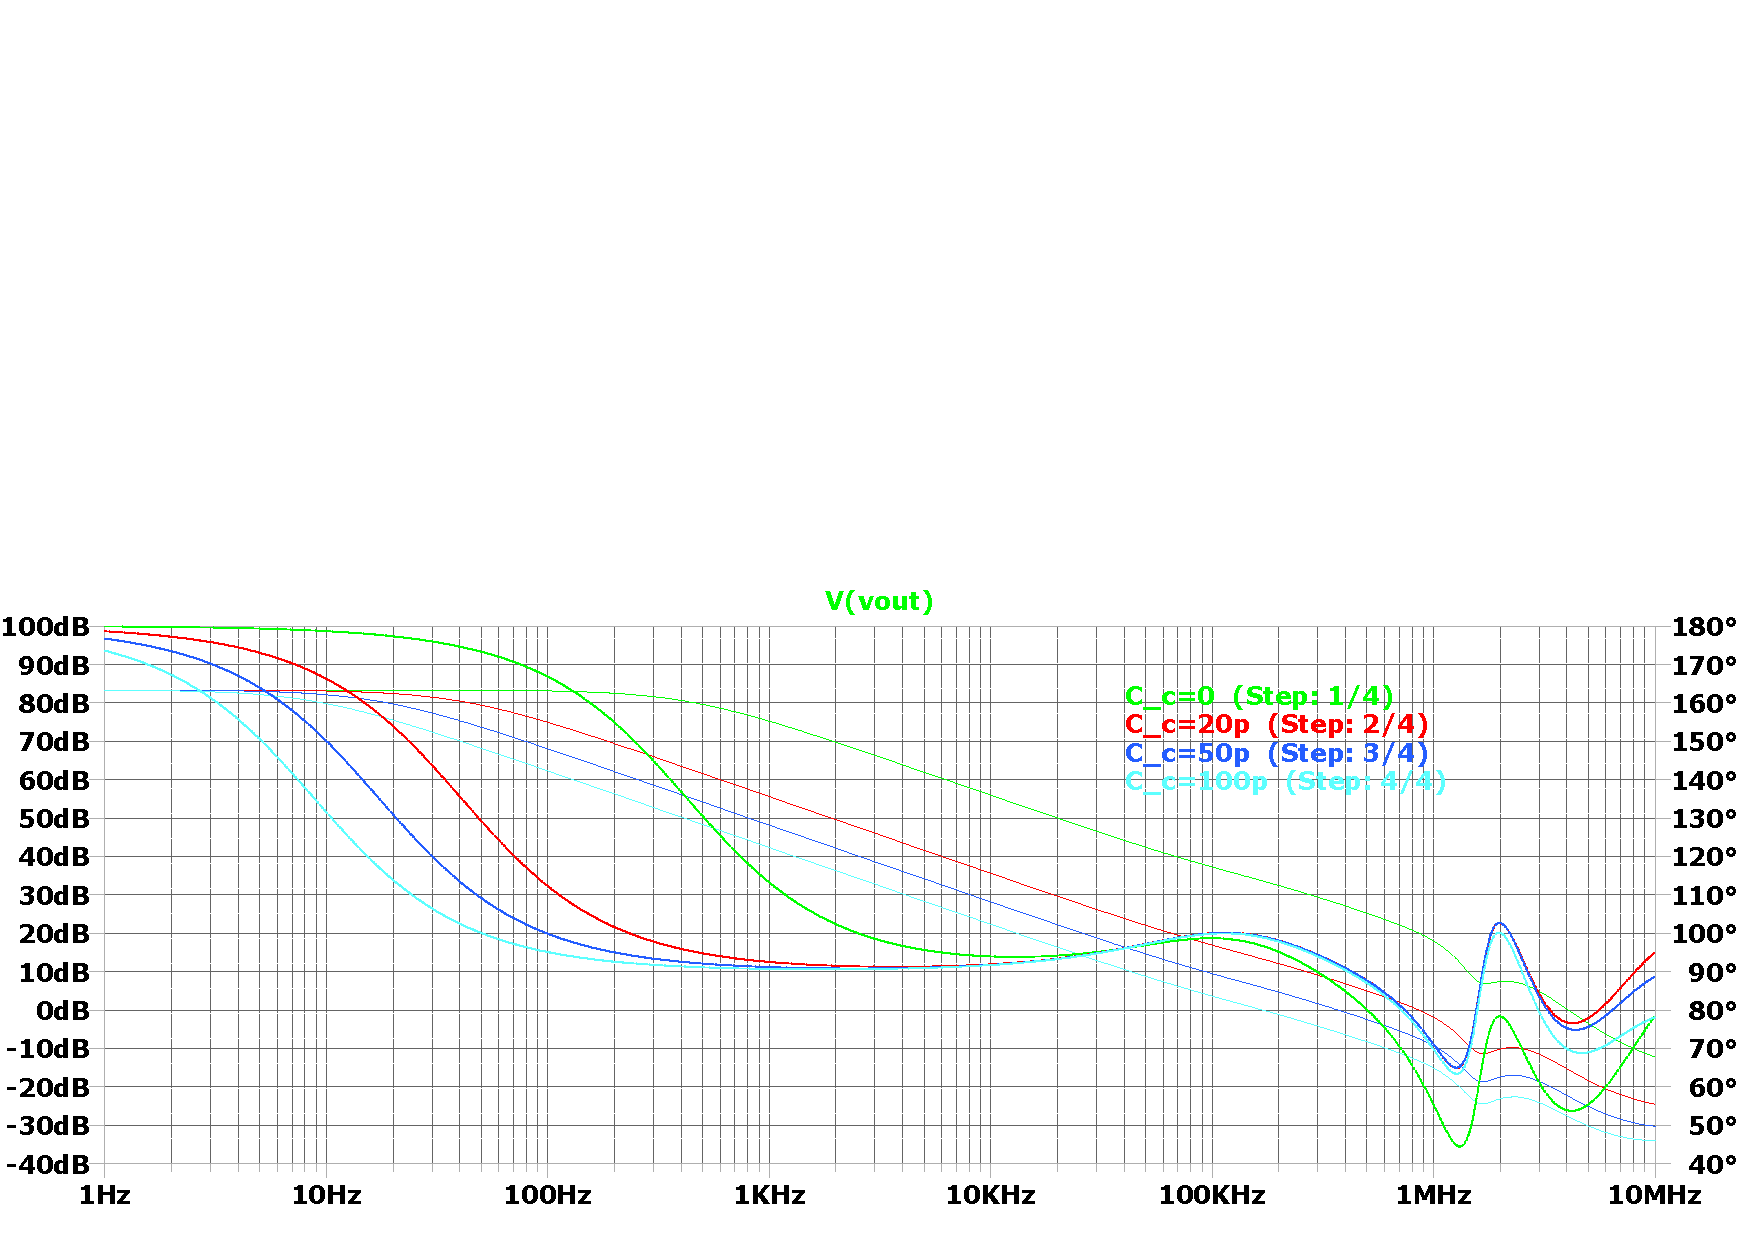
\includegraphics[width=\columnwidth]{LCE-06-07-运放设计/assets/uA741/gain of uA741.pdf}
    \caption{Simulated frequency response of the discrete μA741 (simulation results of Figure \ref{LTspice uA741})}
    \label{simulated uA741 1}
\end{figure}

\begin{figure}[H]\centering
    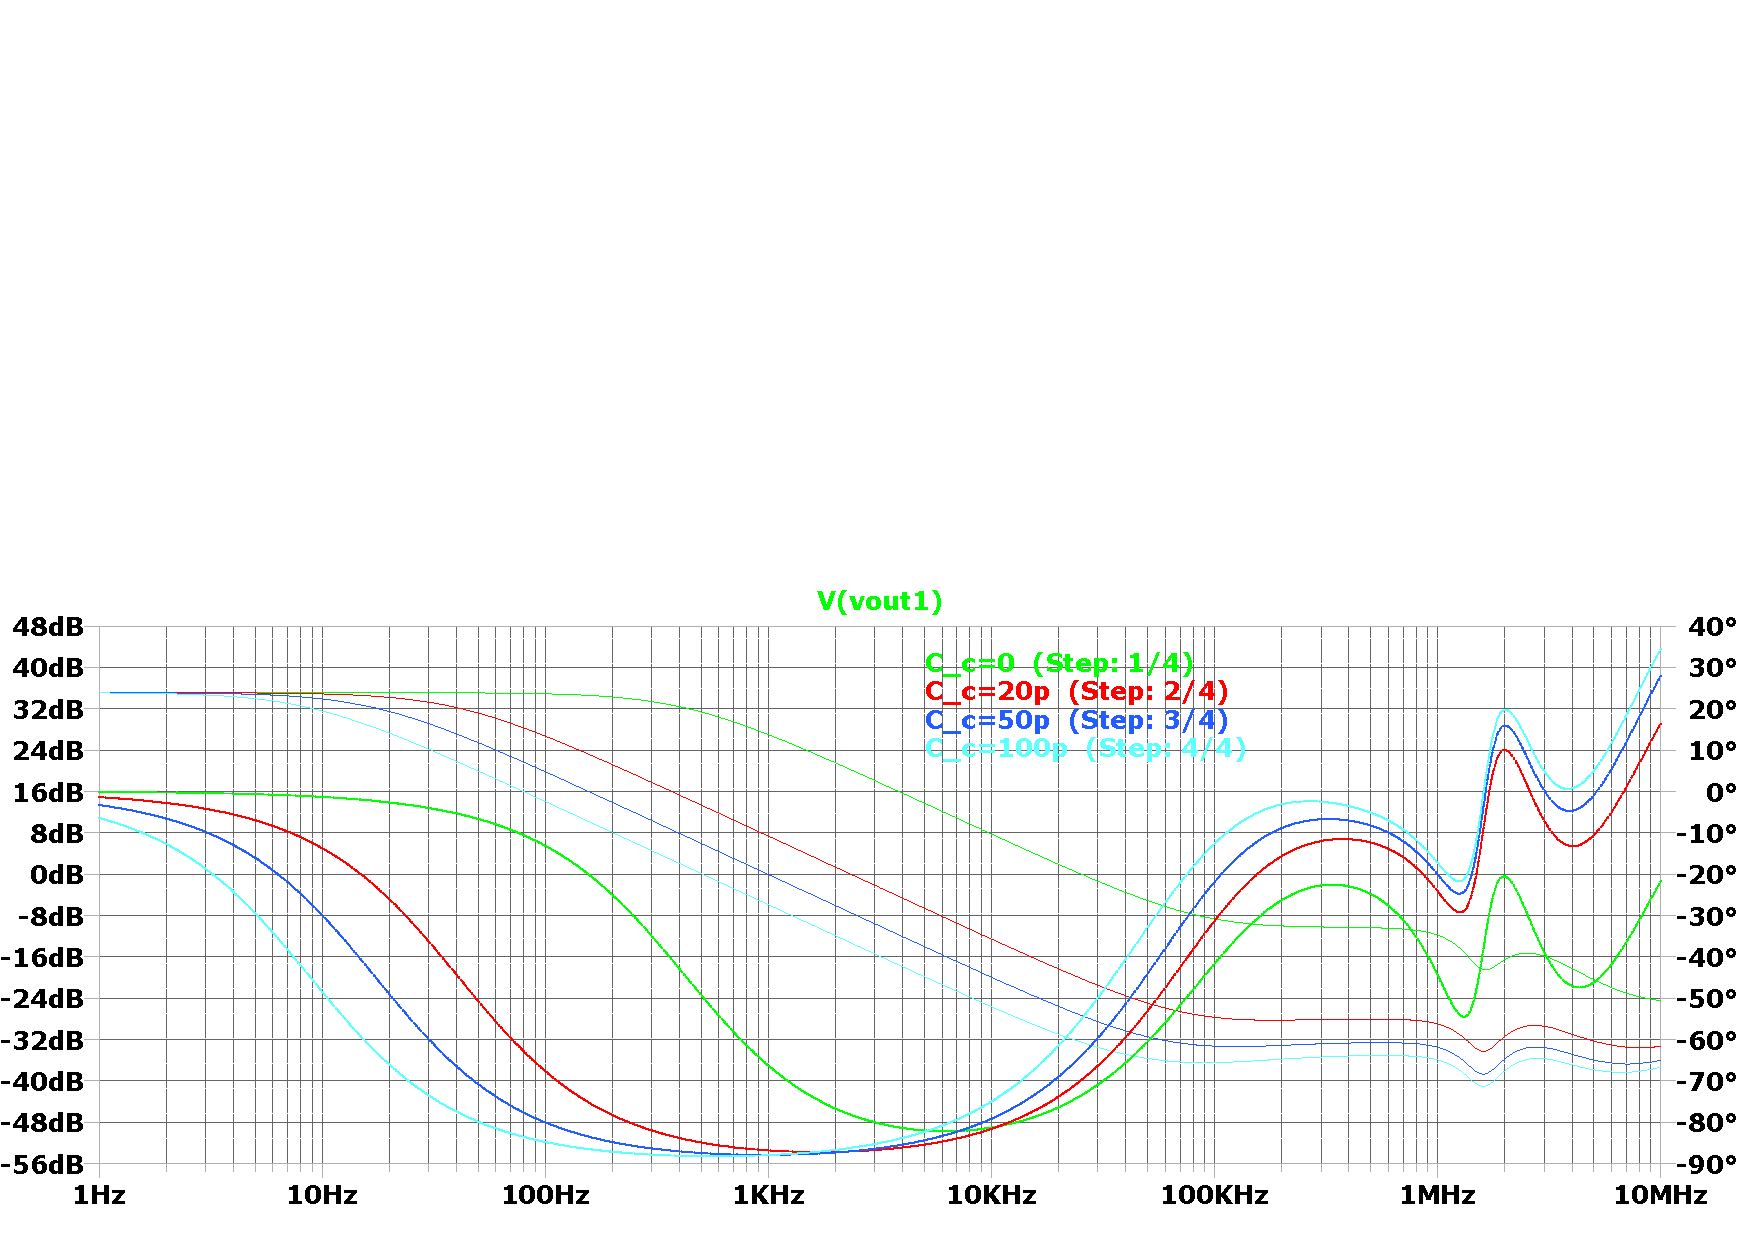
\includegraphics[width=\columnwidth]{LCE-06-07-运放设计/assets/uA741/gain of uA741 (2).pdf}
    \caption{Simulated frequency response of the first stage of the op amp (output of the 1st stage connected to the 2nd stage)}
    \label{simulated uA741 2}
\end{figure}







\section{Experimental Verification}

\subsection{CMOS Op Amp 1}

Config the op amp 1 into unit buffer mode by shorting its output and inverting input nodes. Inject a zero signal or a 5 Vamp sine signal to the non-inverting input node and the output waveform is measured as shown below:

\begin{figure}[H]\centering
    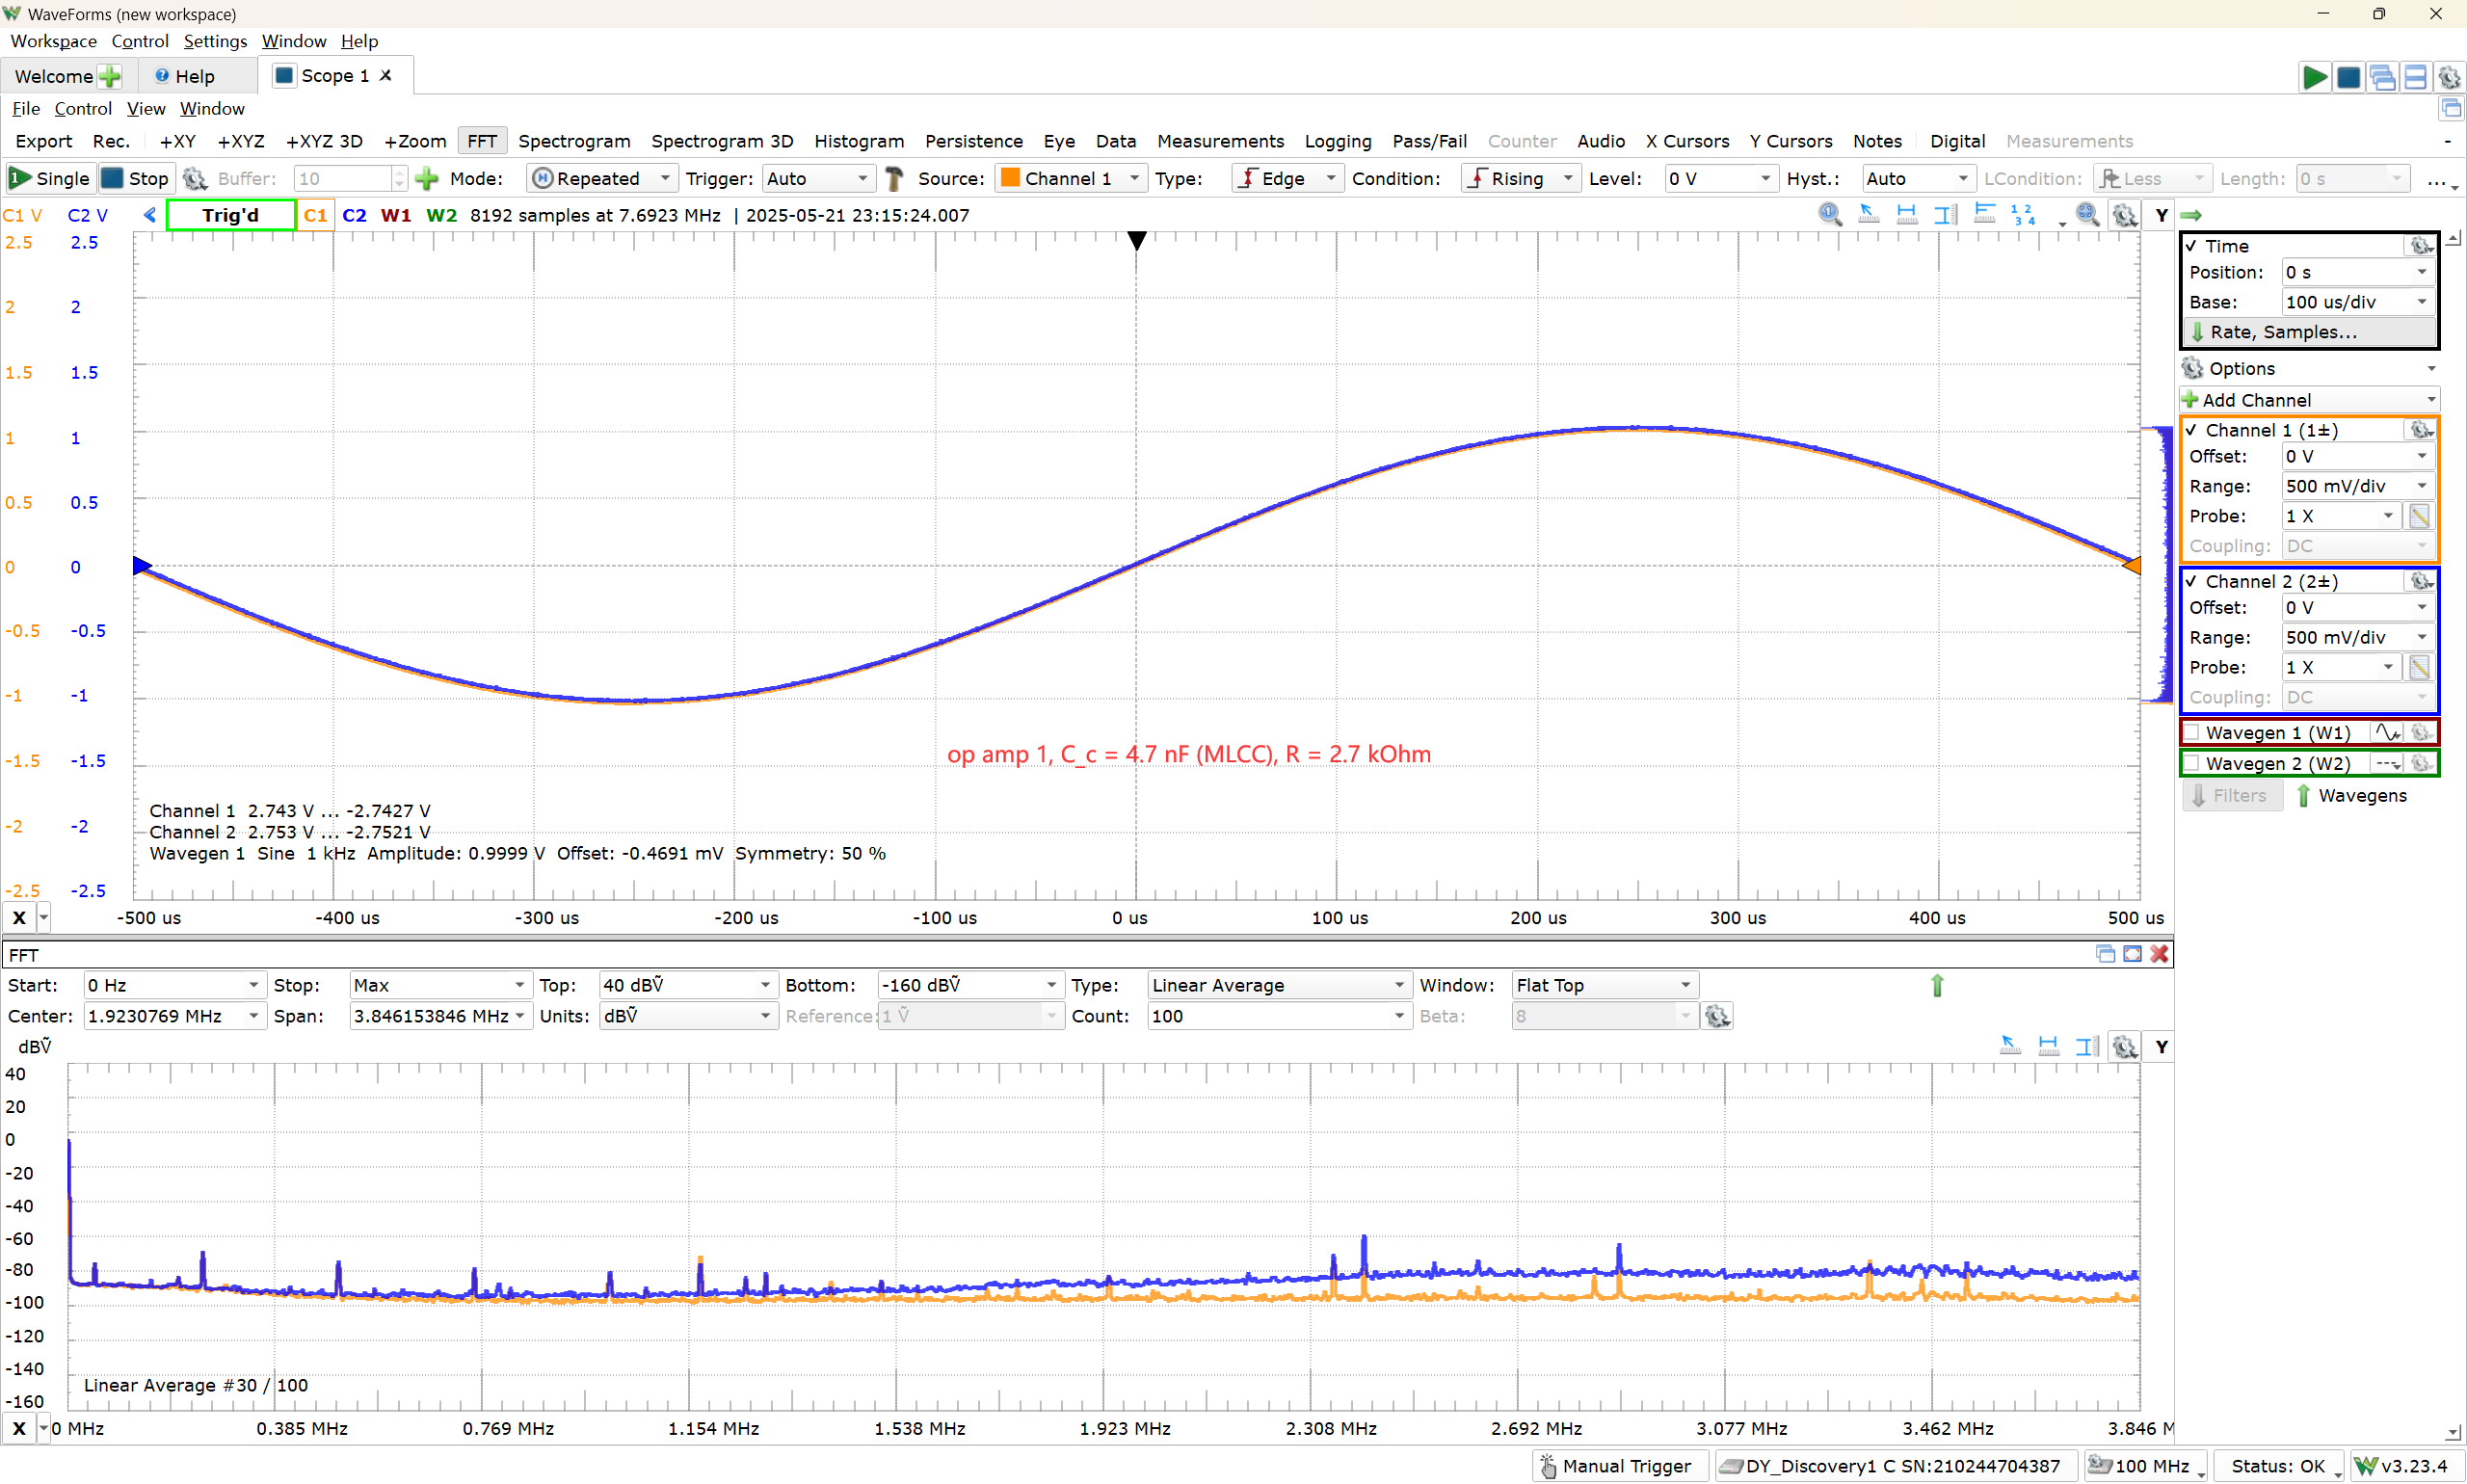
\includegraphics[width=\columnwidth]{LCE-06-07-运放设计/assets/op amp 1/unit 1.png}
    \caption{Unit buffer of CMOS op amp 1 (CS): sine input test; input 5 Vamp @ 1 kHz, CH1 (orange) input, CH2 (blue) output}
\end{figure}

\begin{figure}[H]\centering
    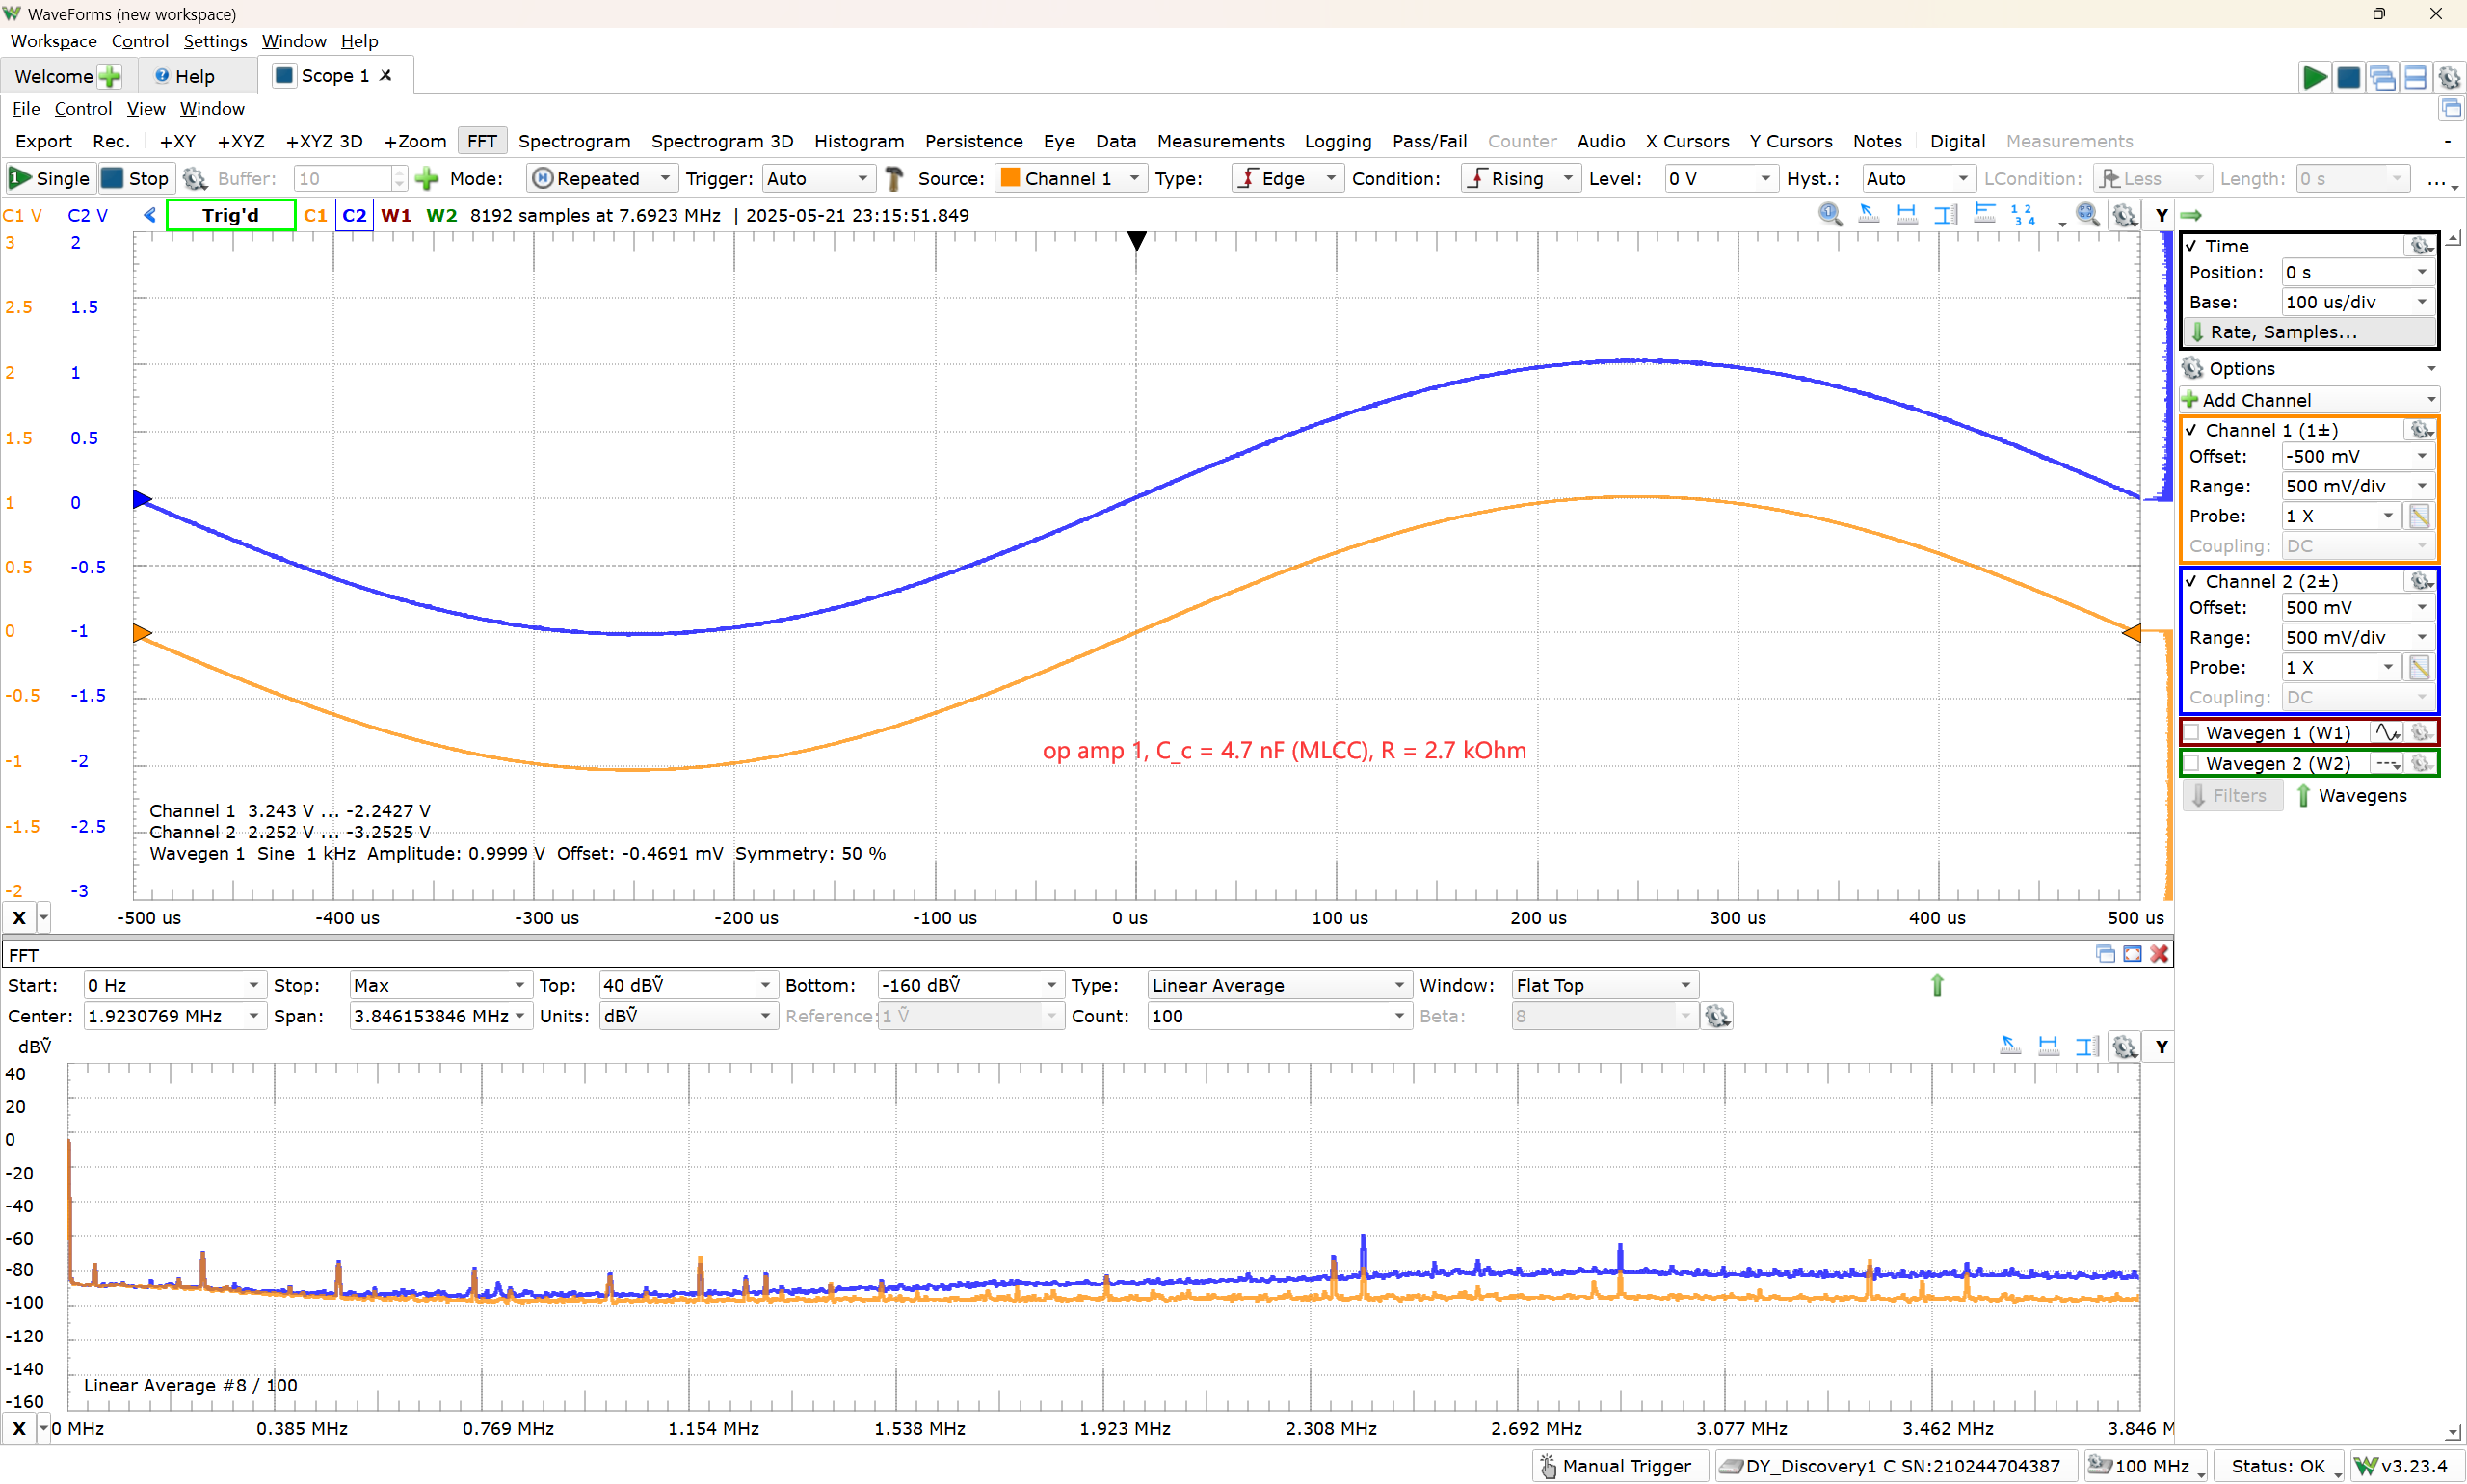
\includegraphics[width=\columnwidth]{LCE-06-07-运放设计/assets/op amp 1/unit 2.png}
    \caption{Unit buffer of CMOS op amp 1 (CS): sine input test; input 5 Vamp @ 1 kHz, CH1 (orange) input, CH2 (blue) output; misaligned display}
\end{figure}

\begin{figure}[H]\centering
    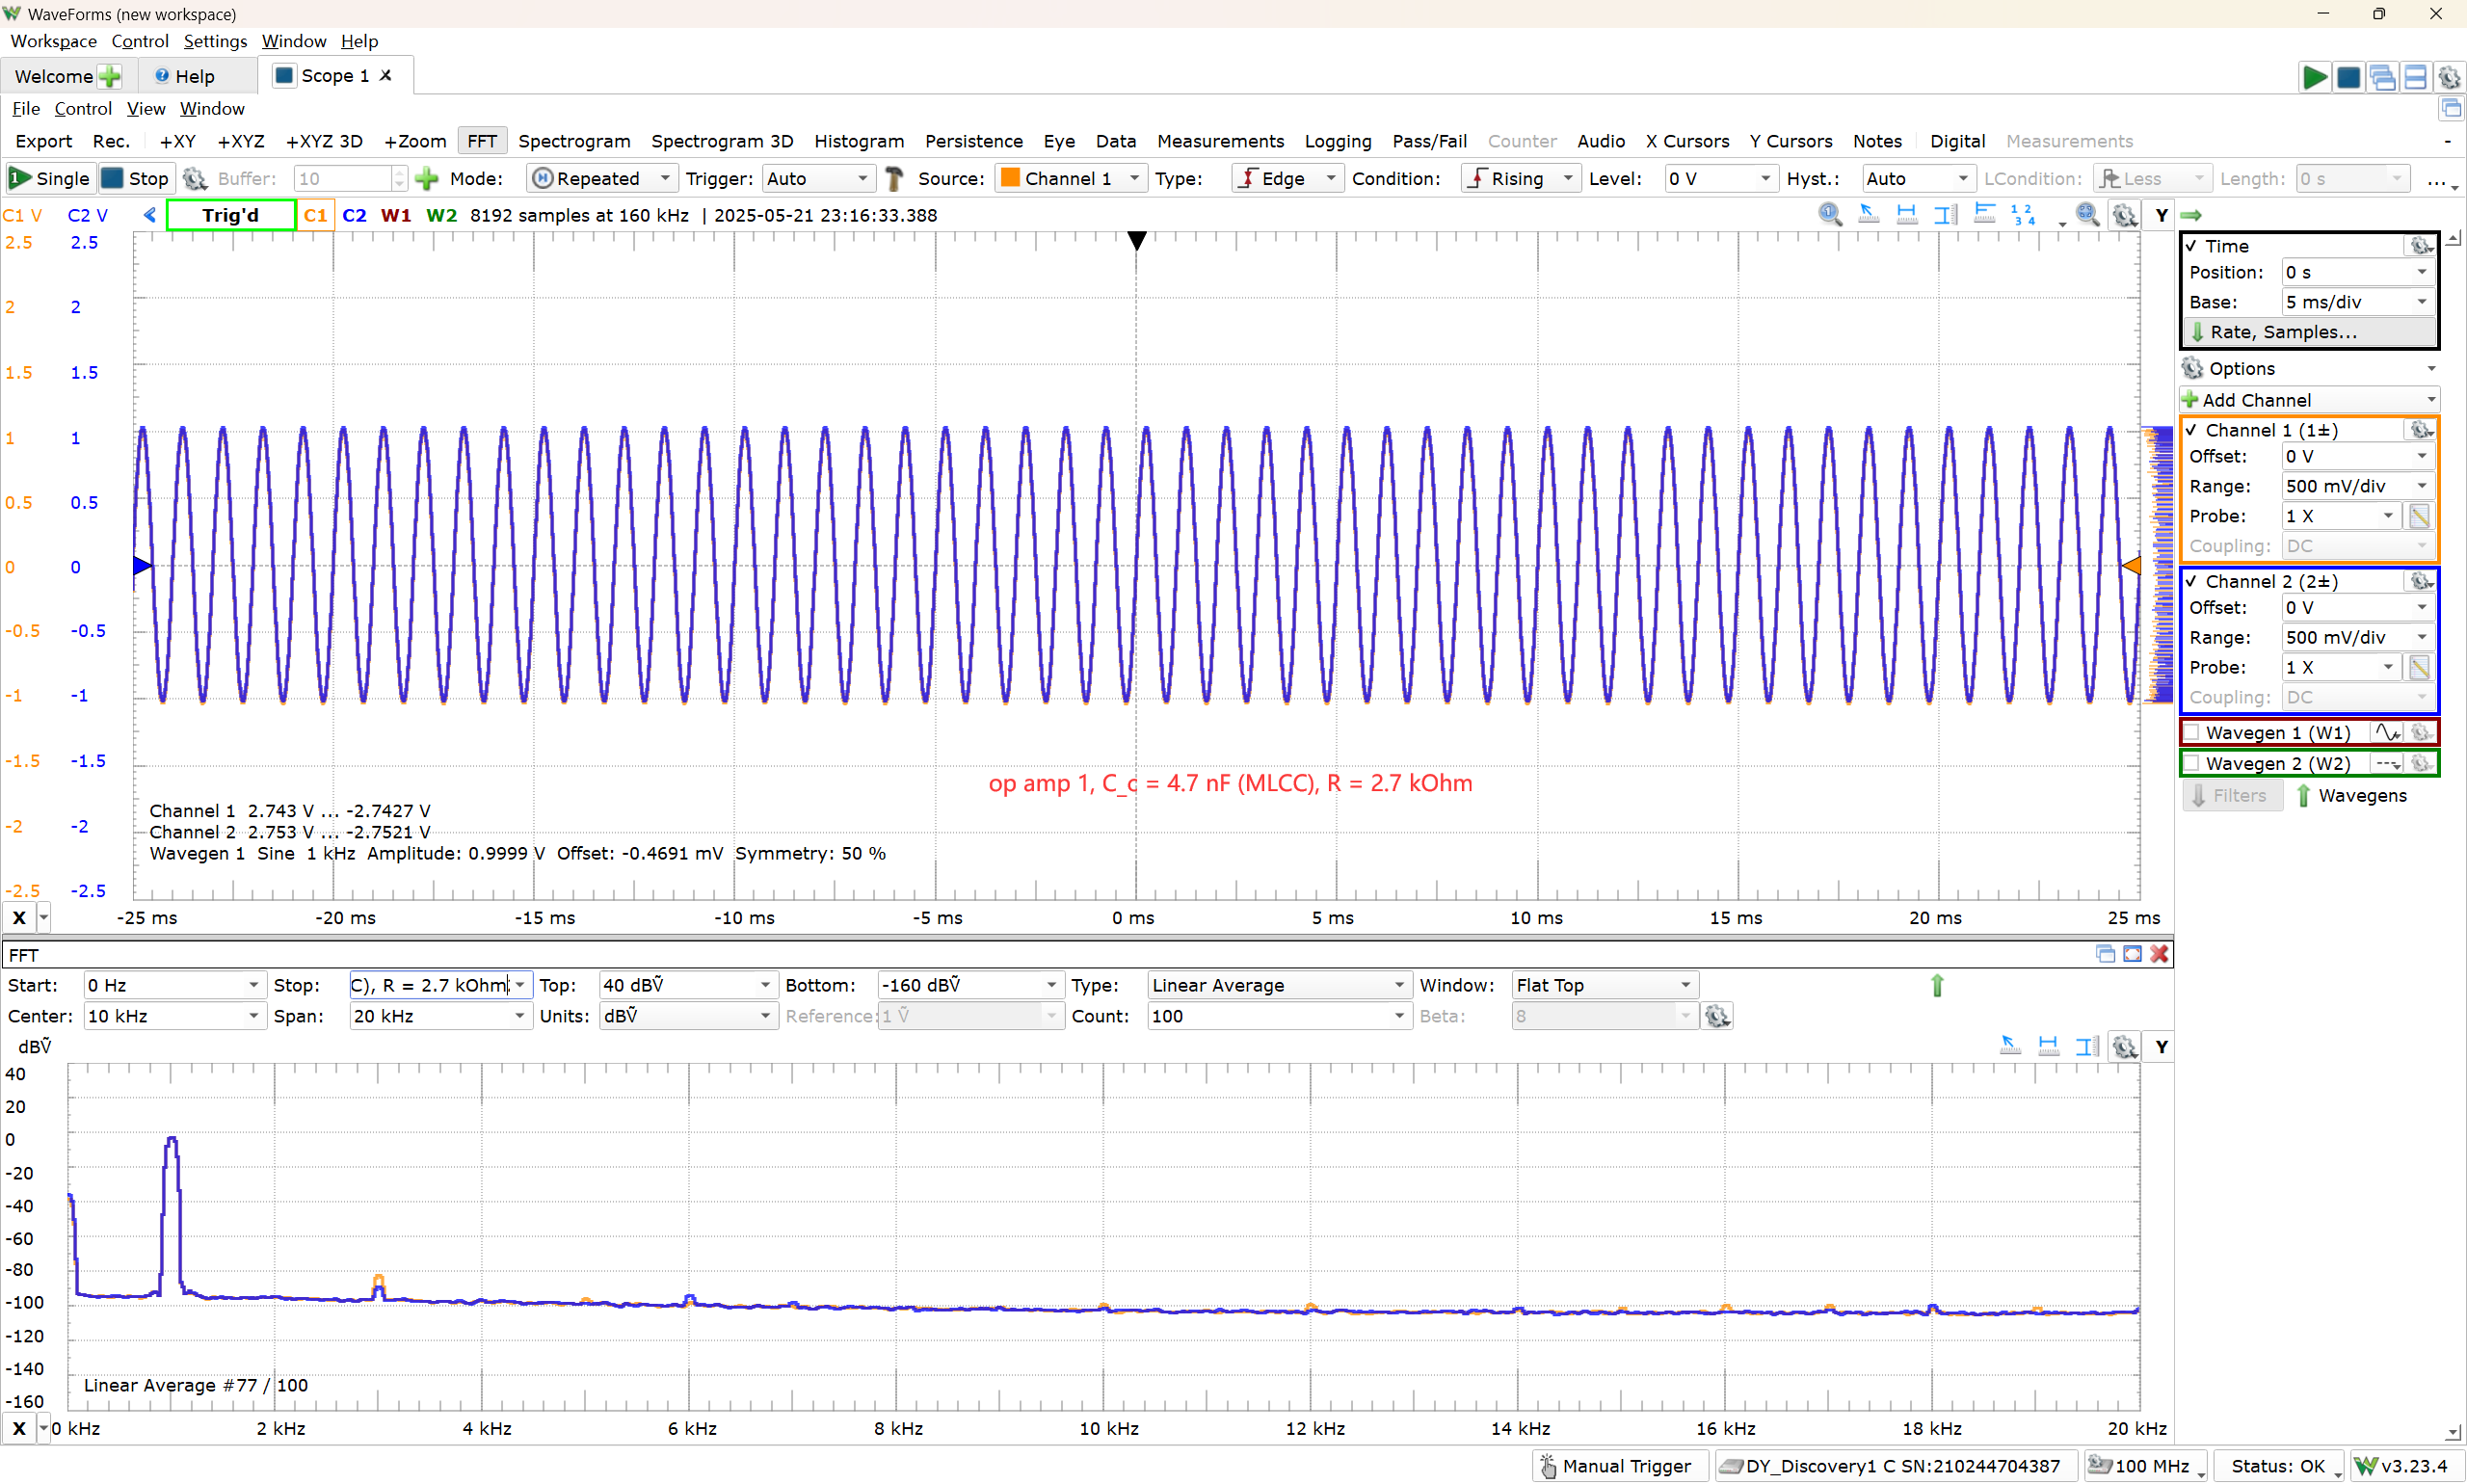
\includegraphics[width=\columnwidth]{LCE-06-07-运放设计/assets/op amp 1/unit 3.png}
    \caption{Unit buffer of CMOS op amp 1 (CS): harmonic distortion test; input 5 Vamp @ 1 kHz, CH1 (orange) input, CH2 (blue) output}
\end{figure}


\subsection{CMOS Op Amp 2}

Similarly, config the op amp 2 into unit buffer and inject the same signal, the output voltage is measured as shown below:

\begin{figure}[H]\centering
    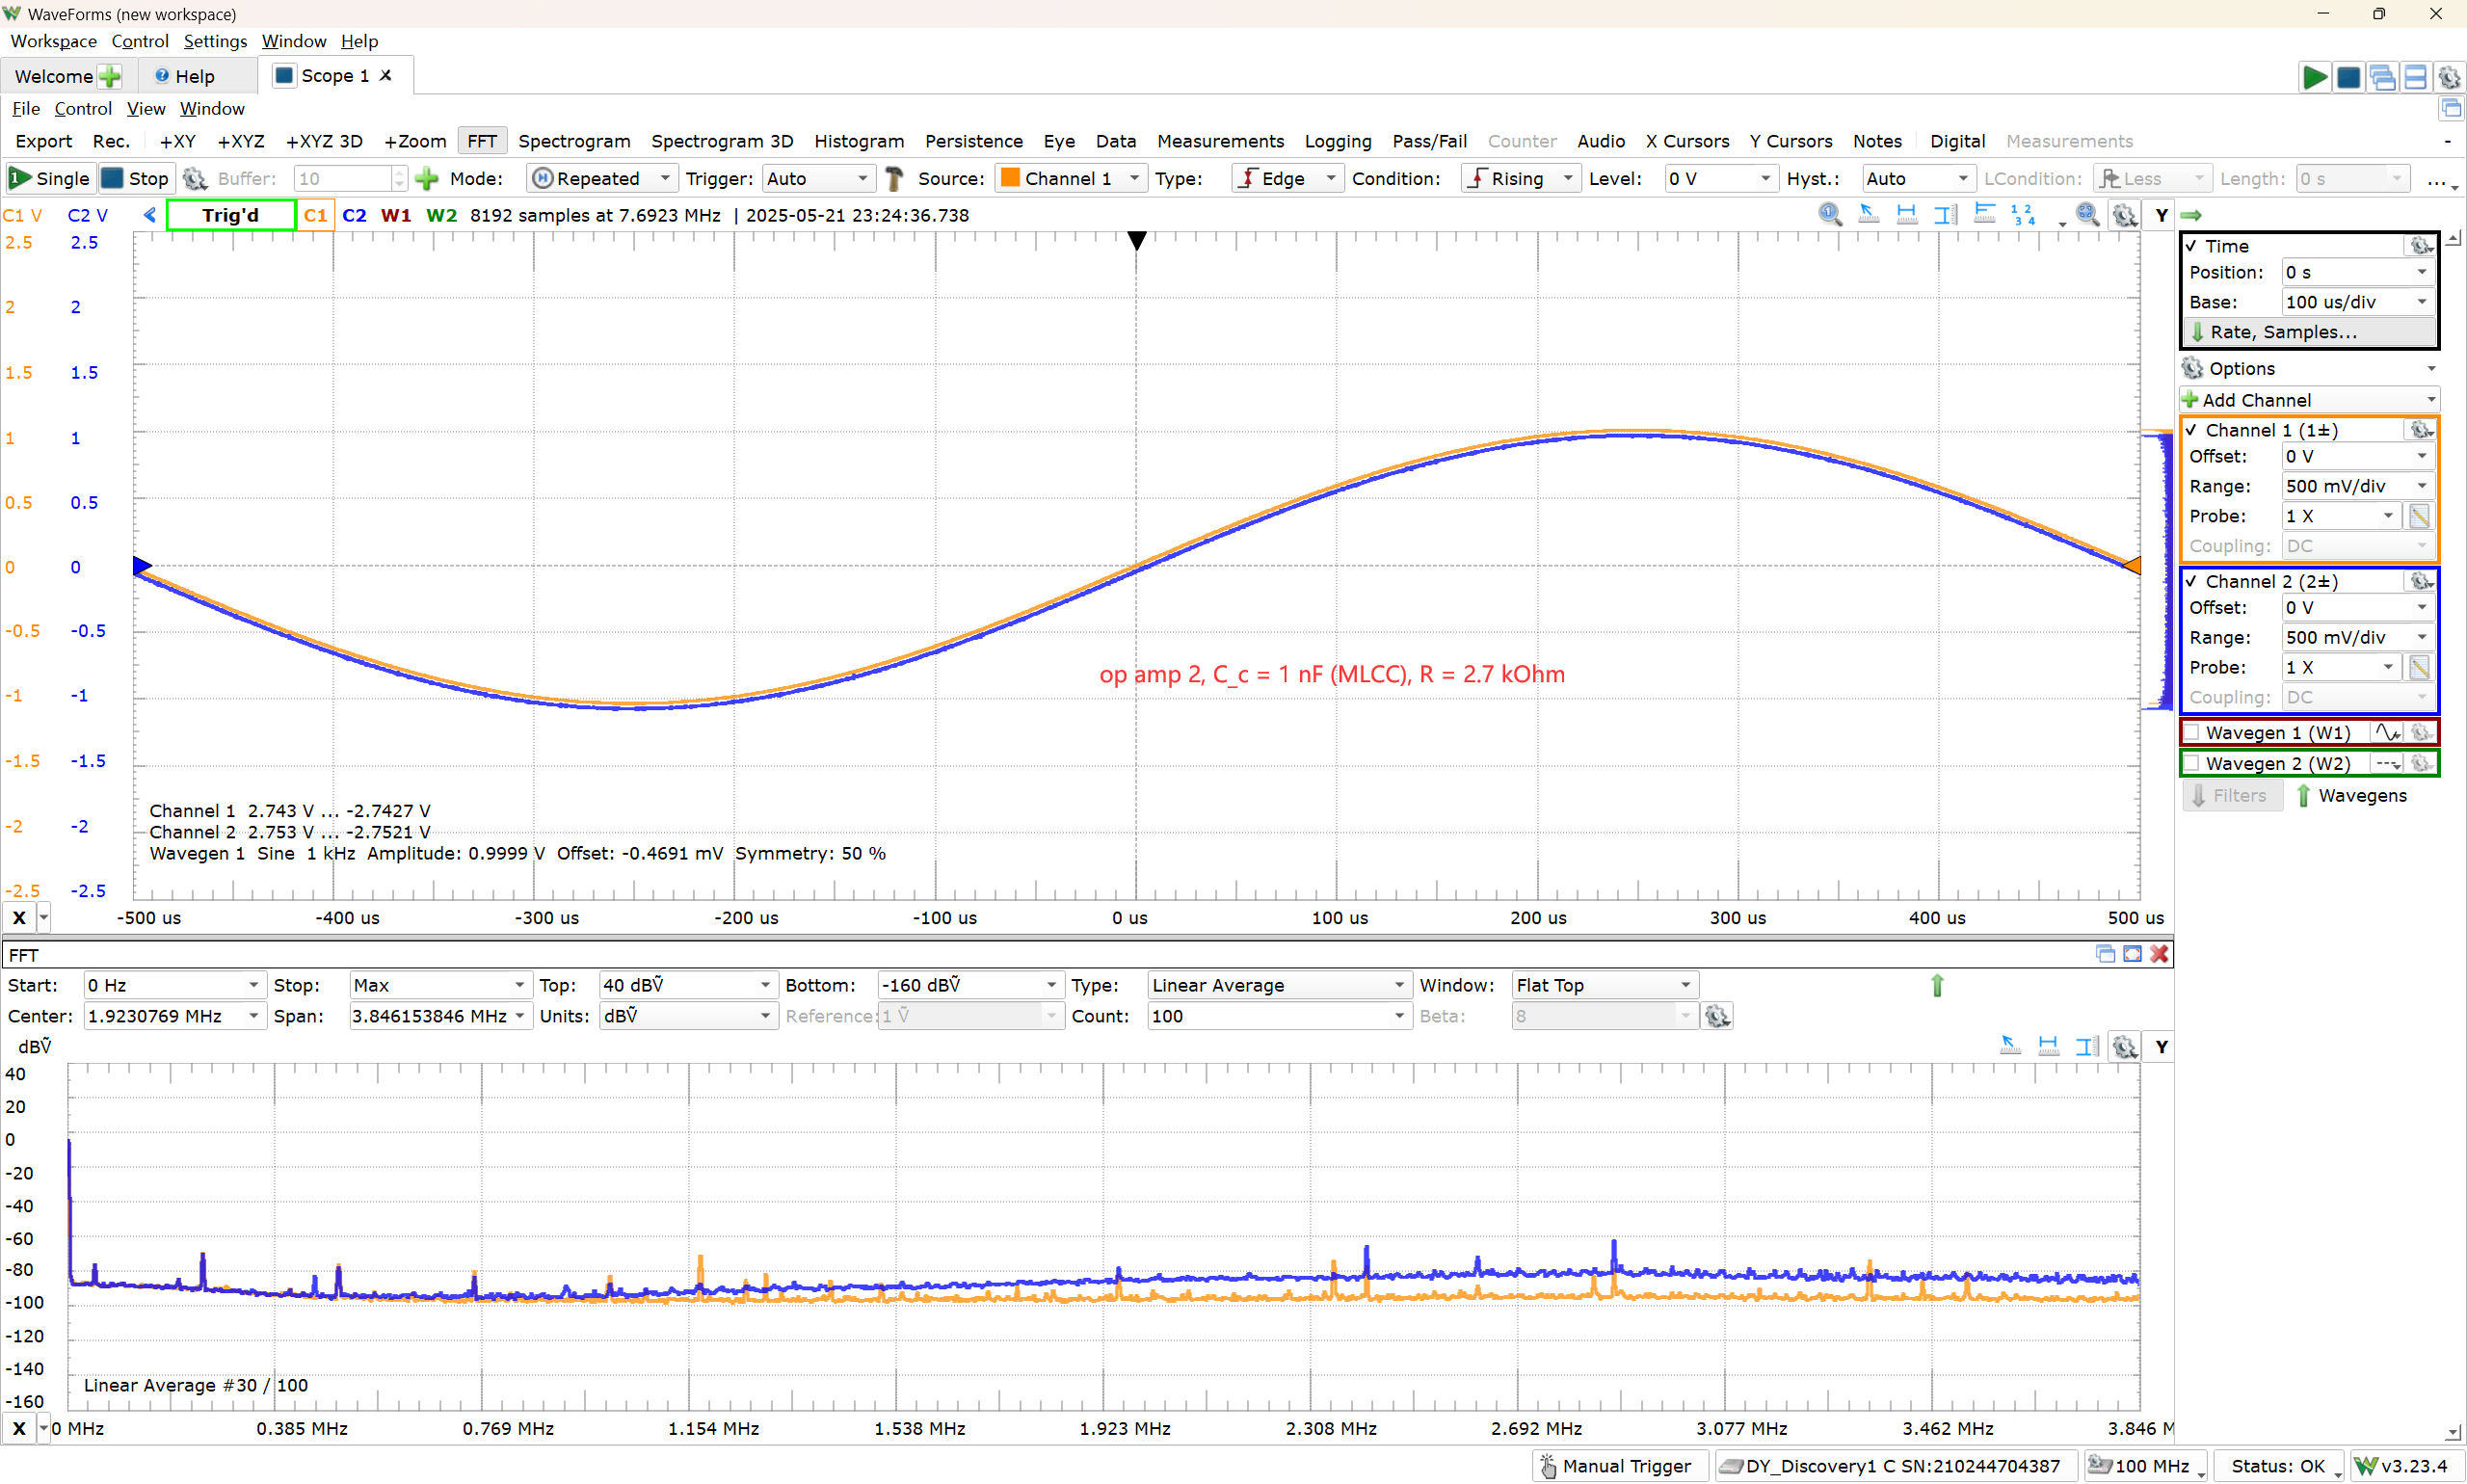
\includegraphics[width=\columnwidth]{LCE-06-07-运放设计/assets/op amp 2/unit 1.png}
    \caption{Unit buffer of CMOS op amp 2 (PP): sine input test; input 5 Vamp @ 1 kHz, CH1 (orange) input, CH2 (blue) output}
\end{figure}

\begin{figure}[H]\centering
    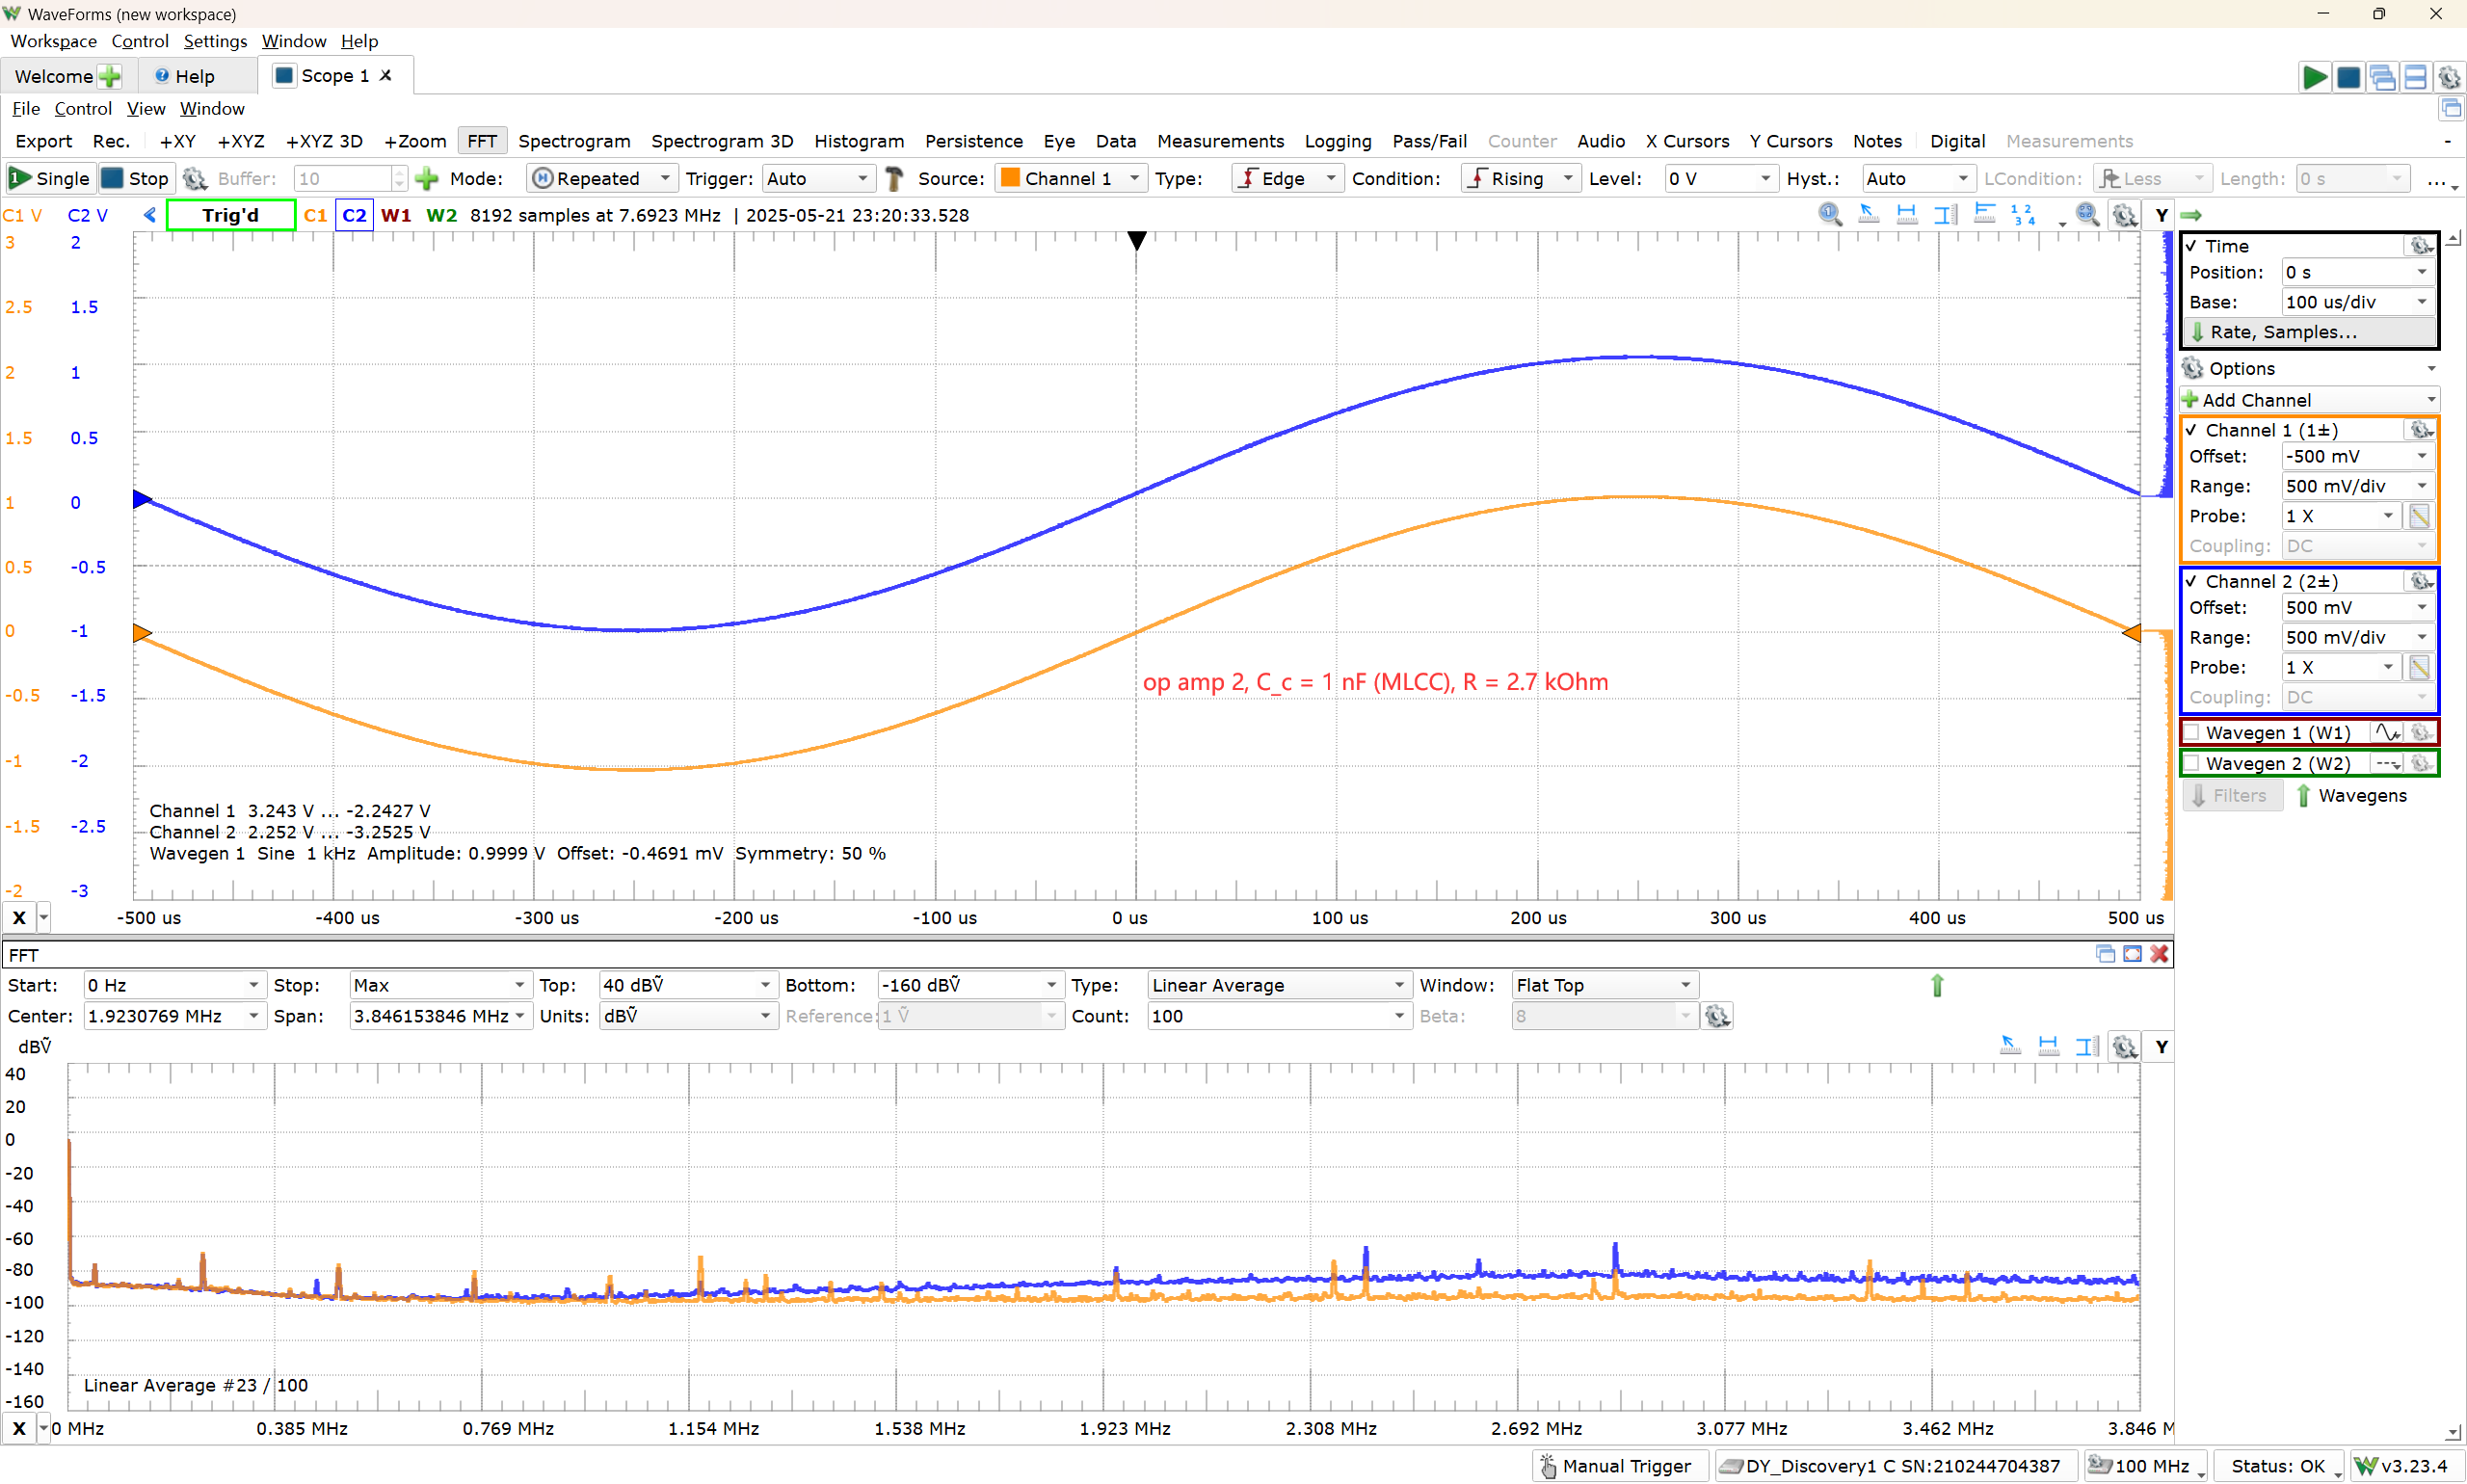
\includegraphics[width=\columnwidth]{LCE-06-07-运放设计/assets/op amp 2/unit 2.png}
    \caption{Unit buffer of CMOS op amp 2 (PP): sine input test; input 5 Vamp @ 1 kHz, CH1 (orange) input, CH2 (blue) output; misaligned display}
\end{figure}

\begin{figure}[H]\centering
    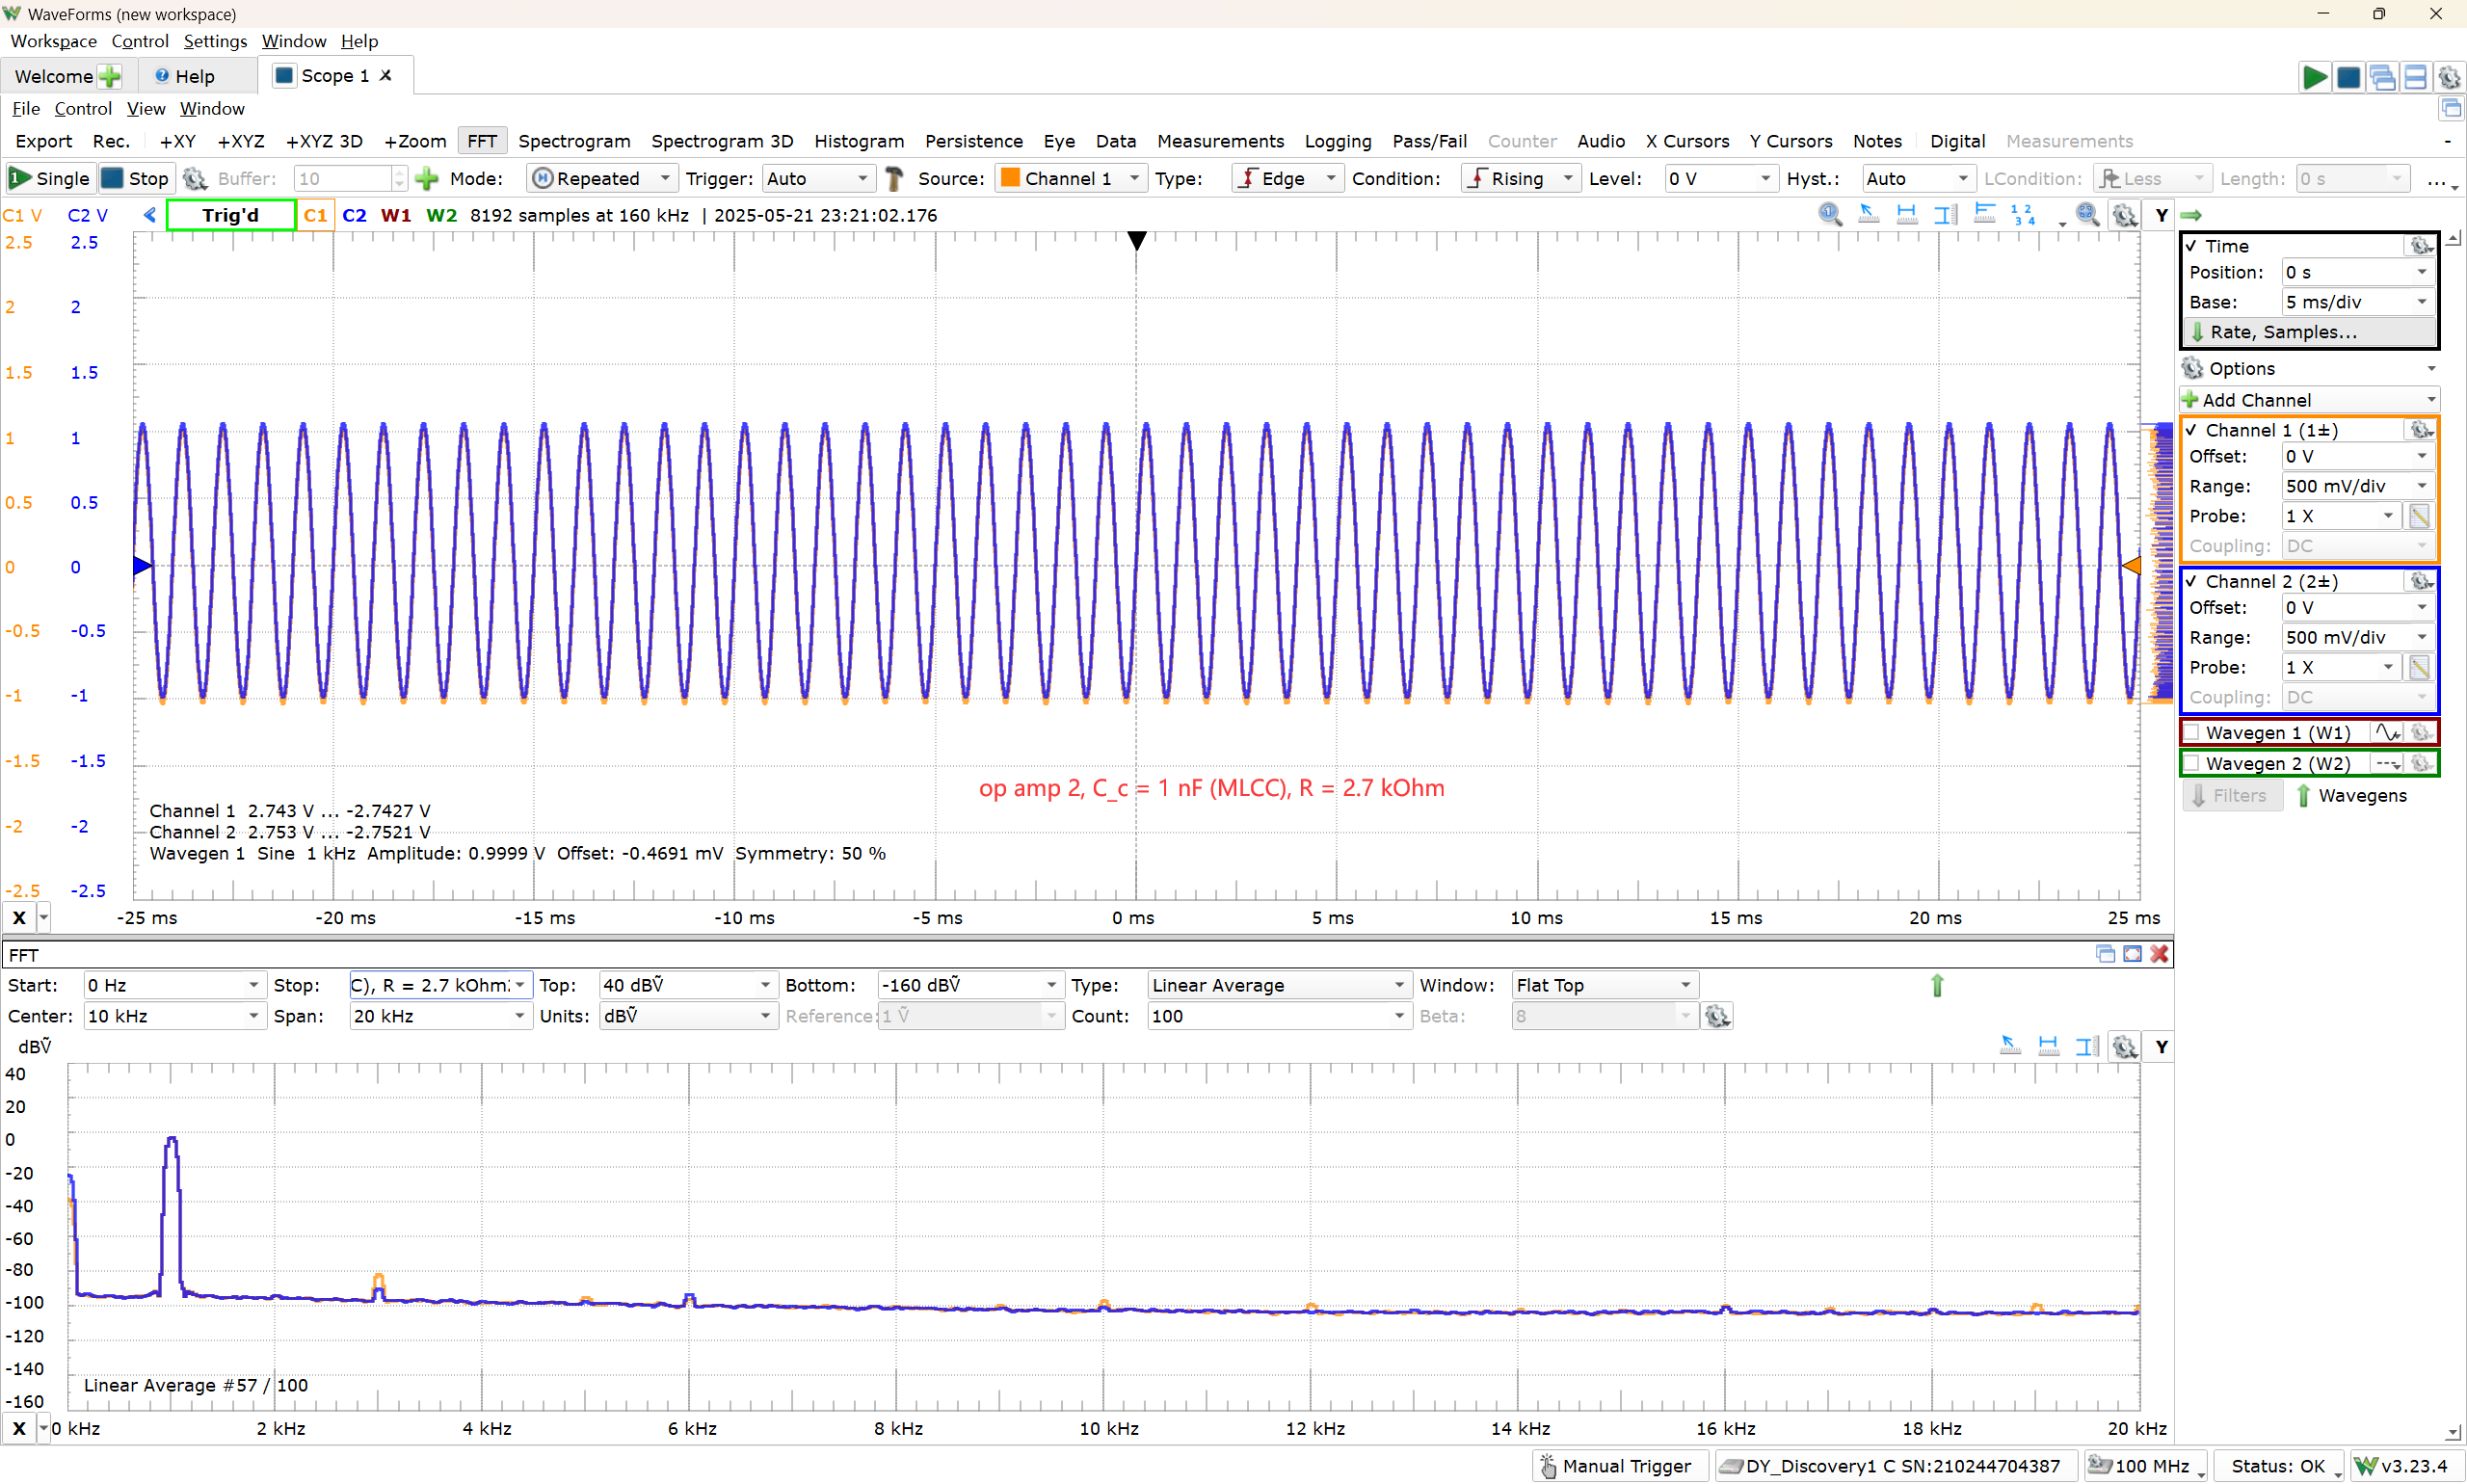
\includegraphics[width=\columnwidth]{LCE-06-07-运放设计/assets/op amp 2/unit 3.png}
    \caption{Unit buffer of CMOS op amp 2 (PP): harmonic distortion test; input 5 Vamp @ 1 kHz, CH1 (orange) input, CH2 (blue) output}
\end{figure}

\subsection{μA741 using Discrete BJTs}
\vspace*{-2mm}
\subsubsection{Zero Input Test}
\vspace*{-3.5mm}
\begin{figure}[H]\centering
    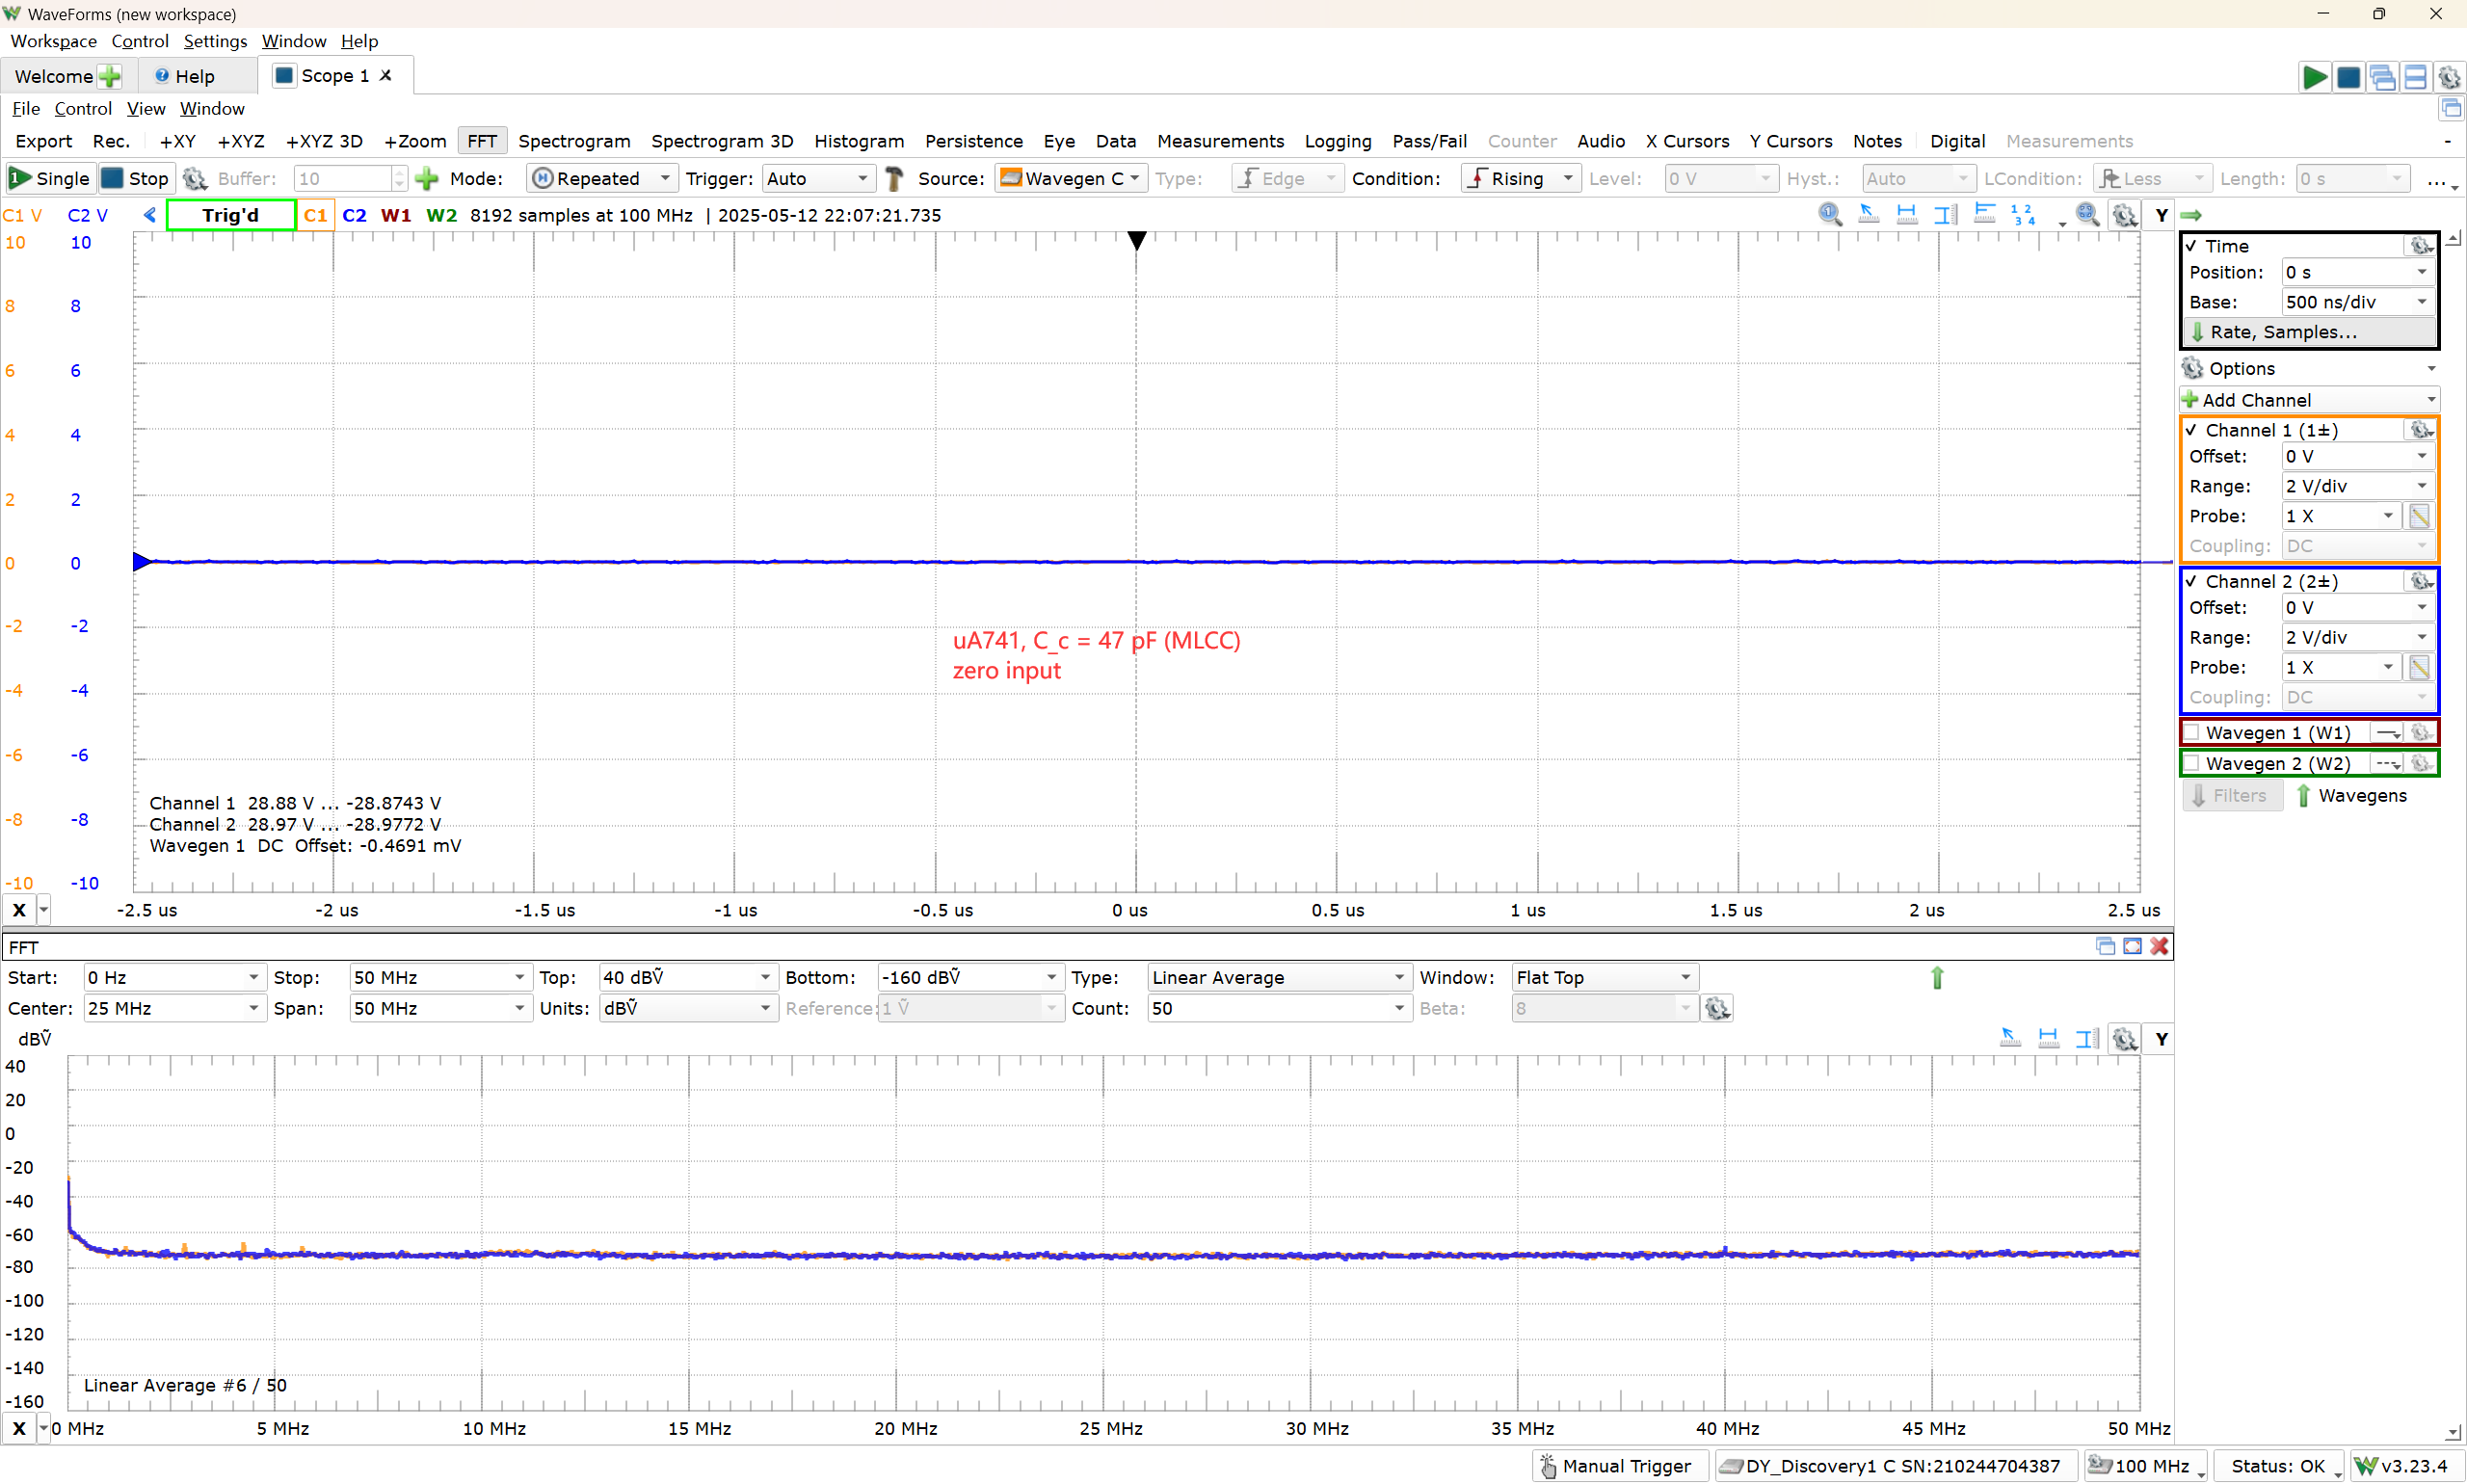
\includegraphics[width=\columnwidth]{LCE-06-07-运放设计/assets/uA741/test/zero input.png}\vspace*{-2mm}
    \caption{Discrete uA741: zero input noise test; CH1 (orange) input, CH2 (blue) output}
\end{figure}
\vspace*{-2mm}
\subsubsection{Unit Buffer}
\vspace*{-3.5mm}
\begin{figure}[H]\centering
    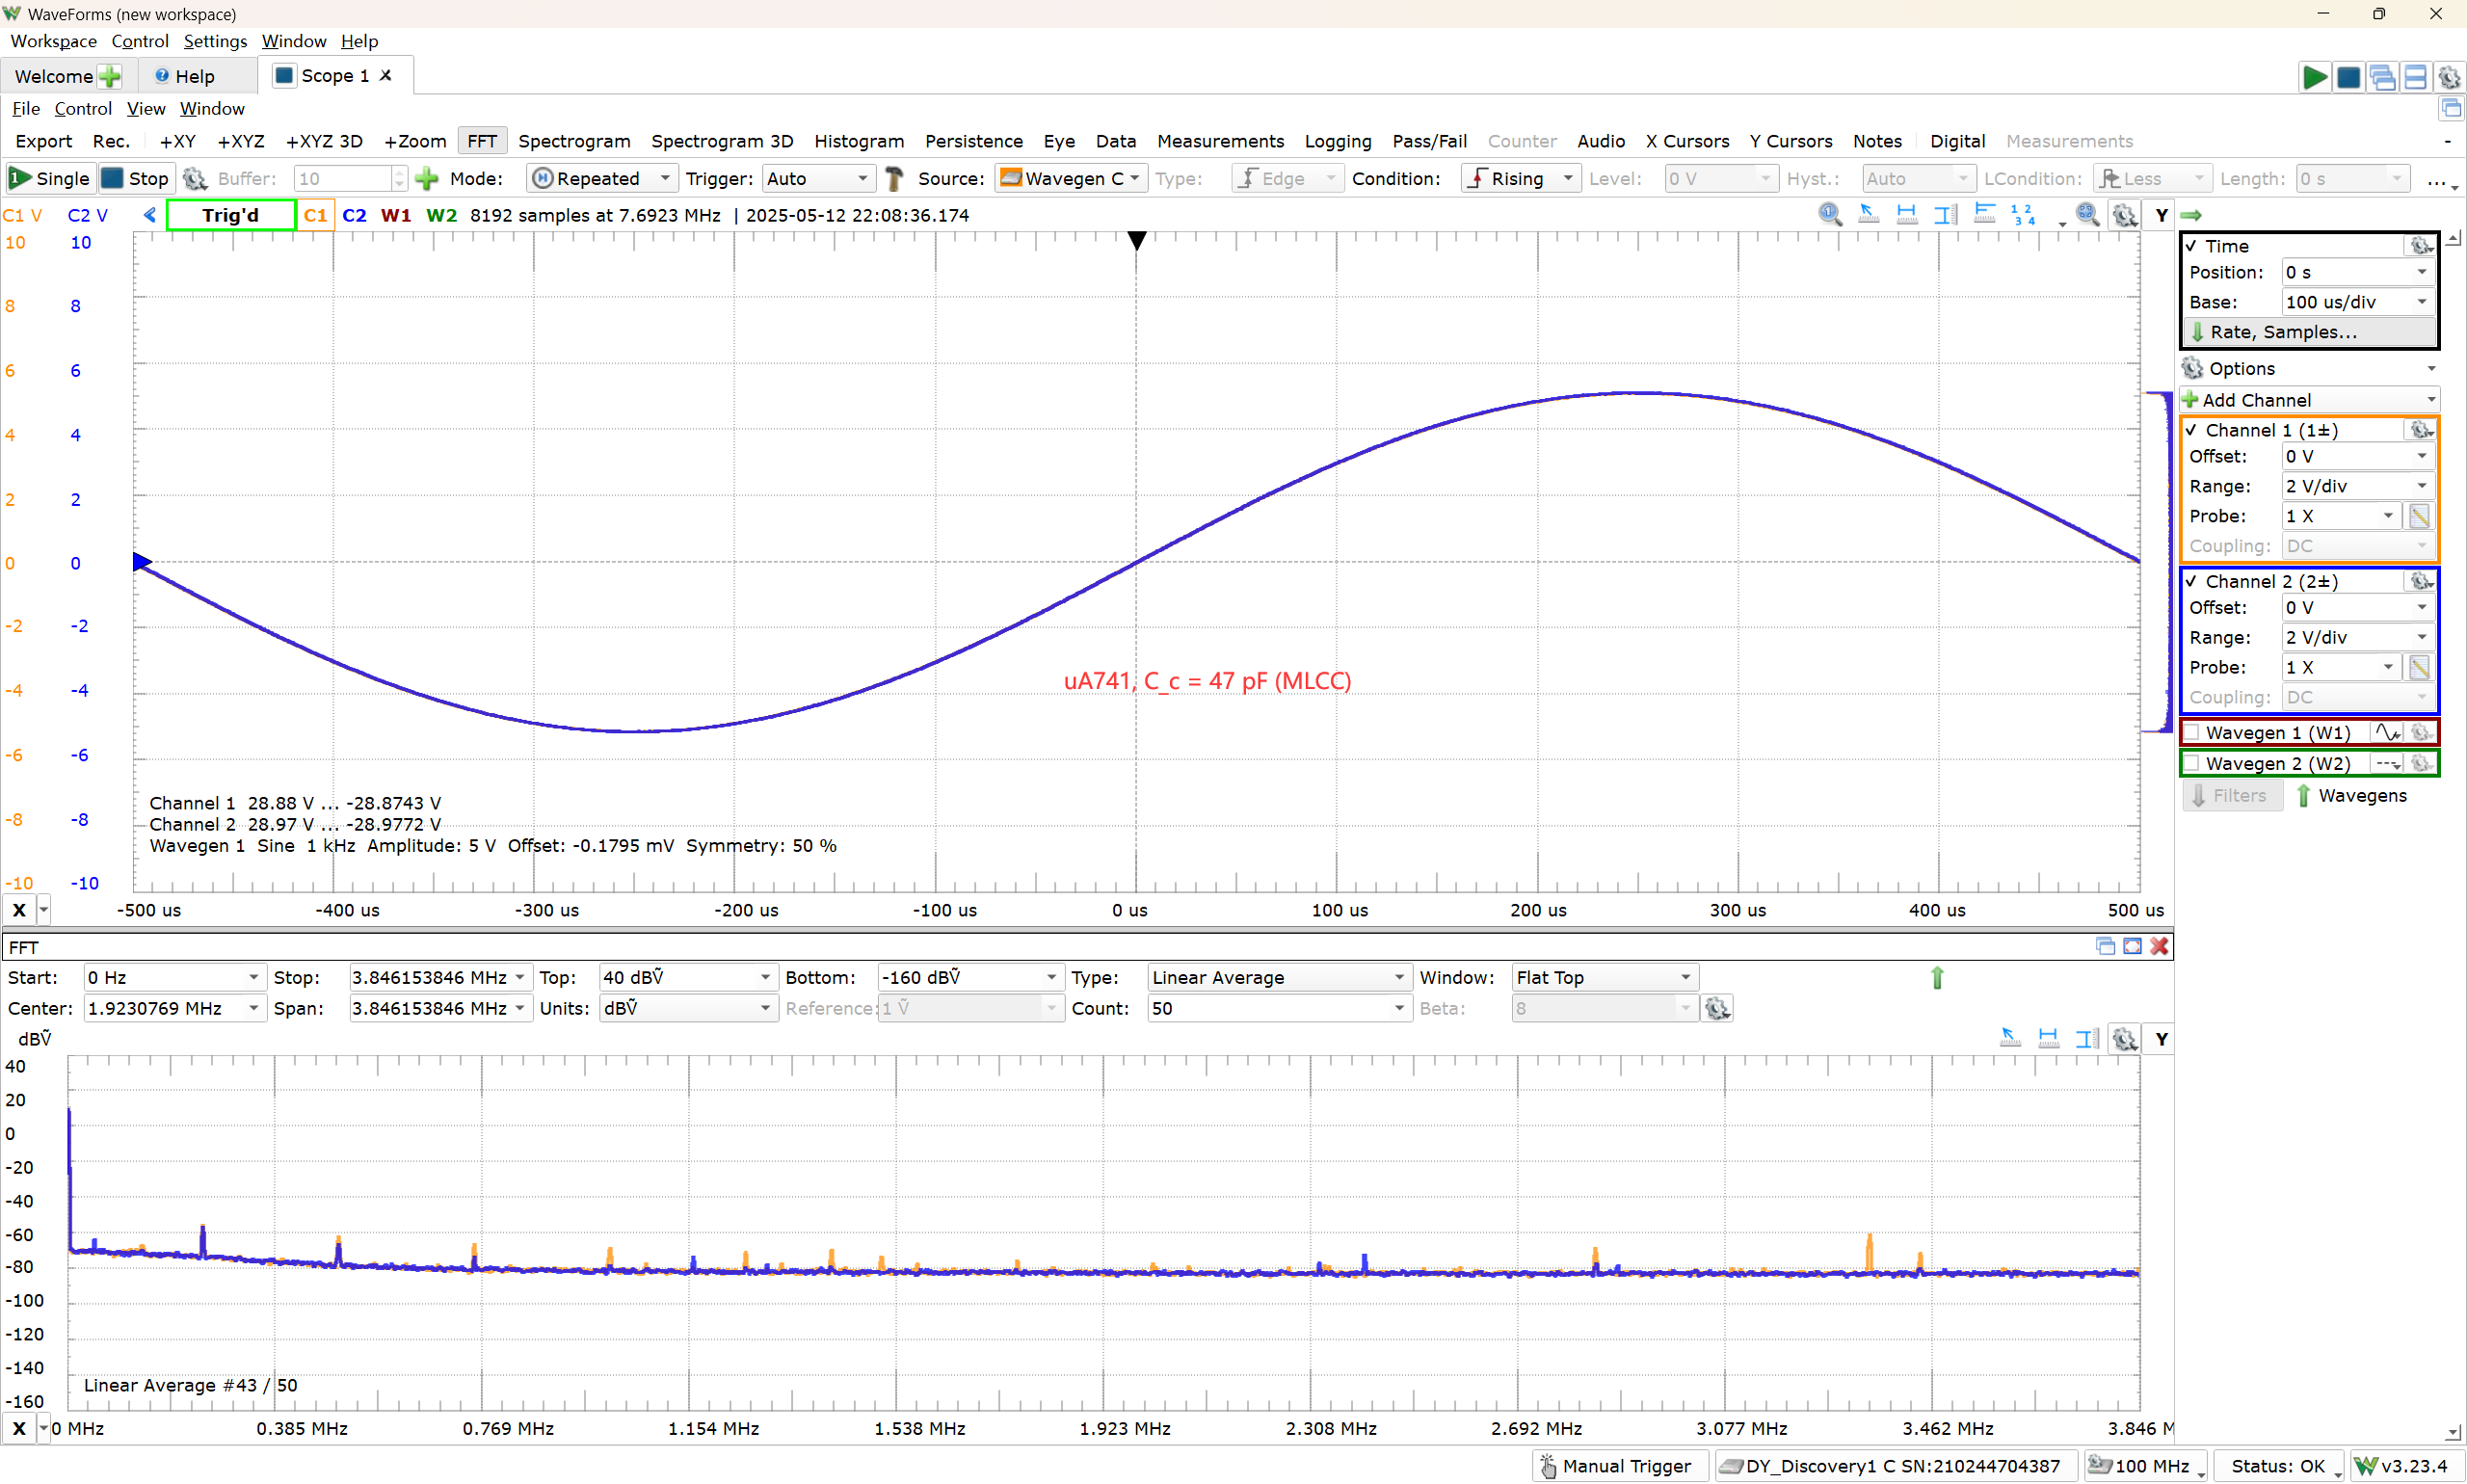
\includegraphics[width=\columnwidth]{LCE-06-07-运放设计/assets/uA741/test/unit buffer 1.png}\vspace*{-2mm}
    \caption{uA741 unit buffer: sine input test; input 5 Vamp @ 1 kHz, CH1 (orange) input, CH2 (blue) output}
\end{figure}

\begin{figure}[H]\centering
    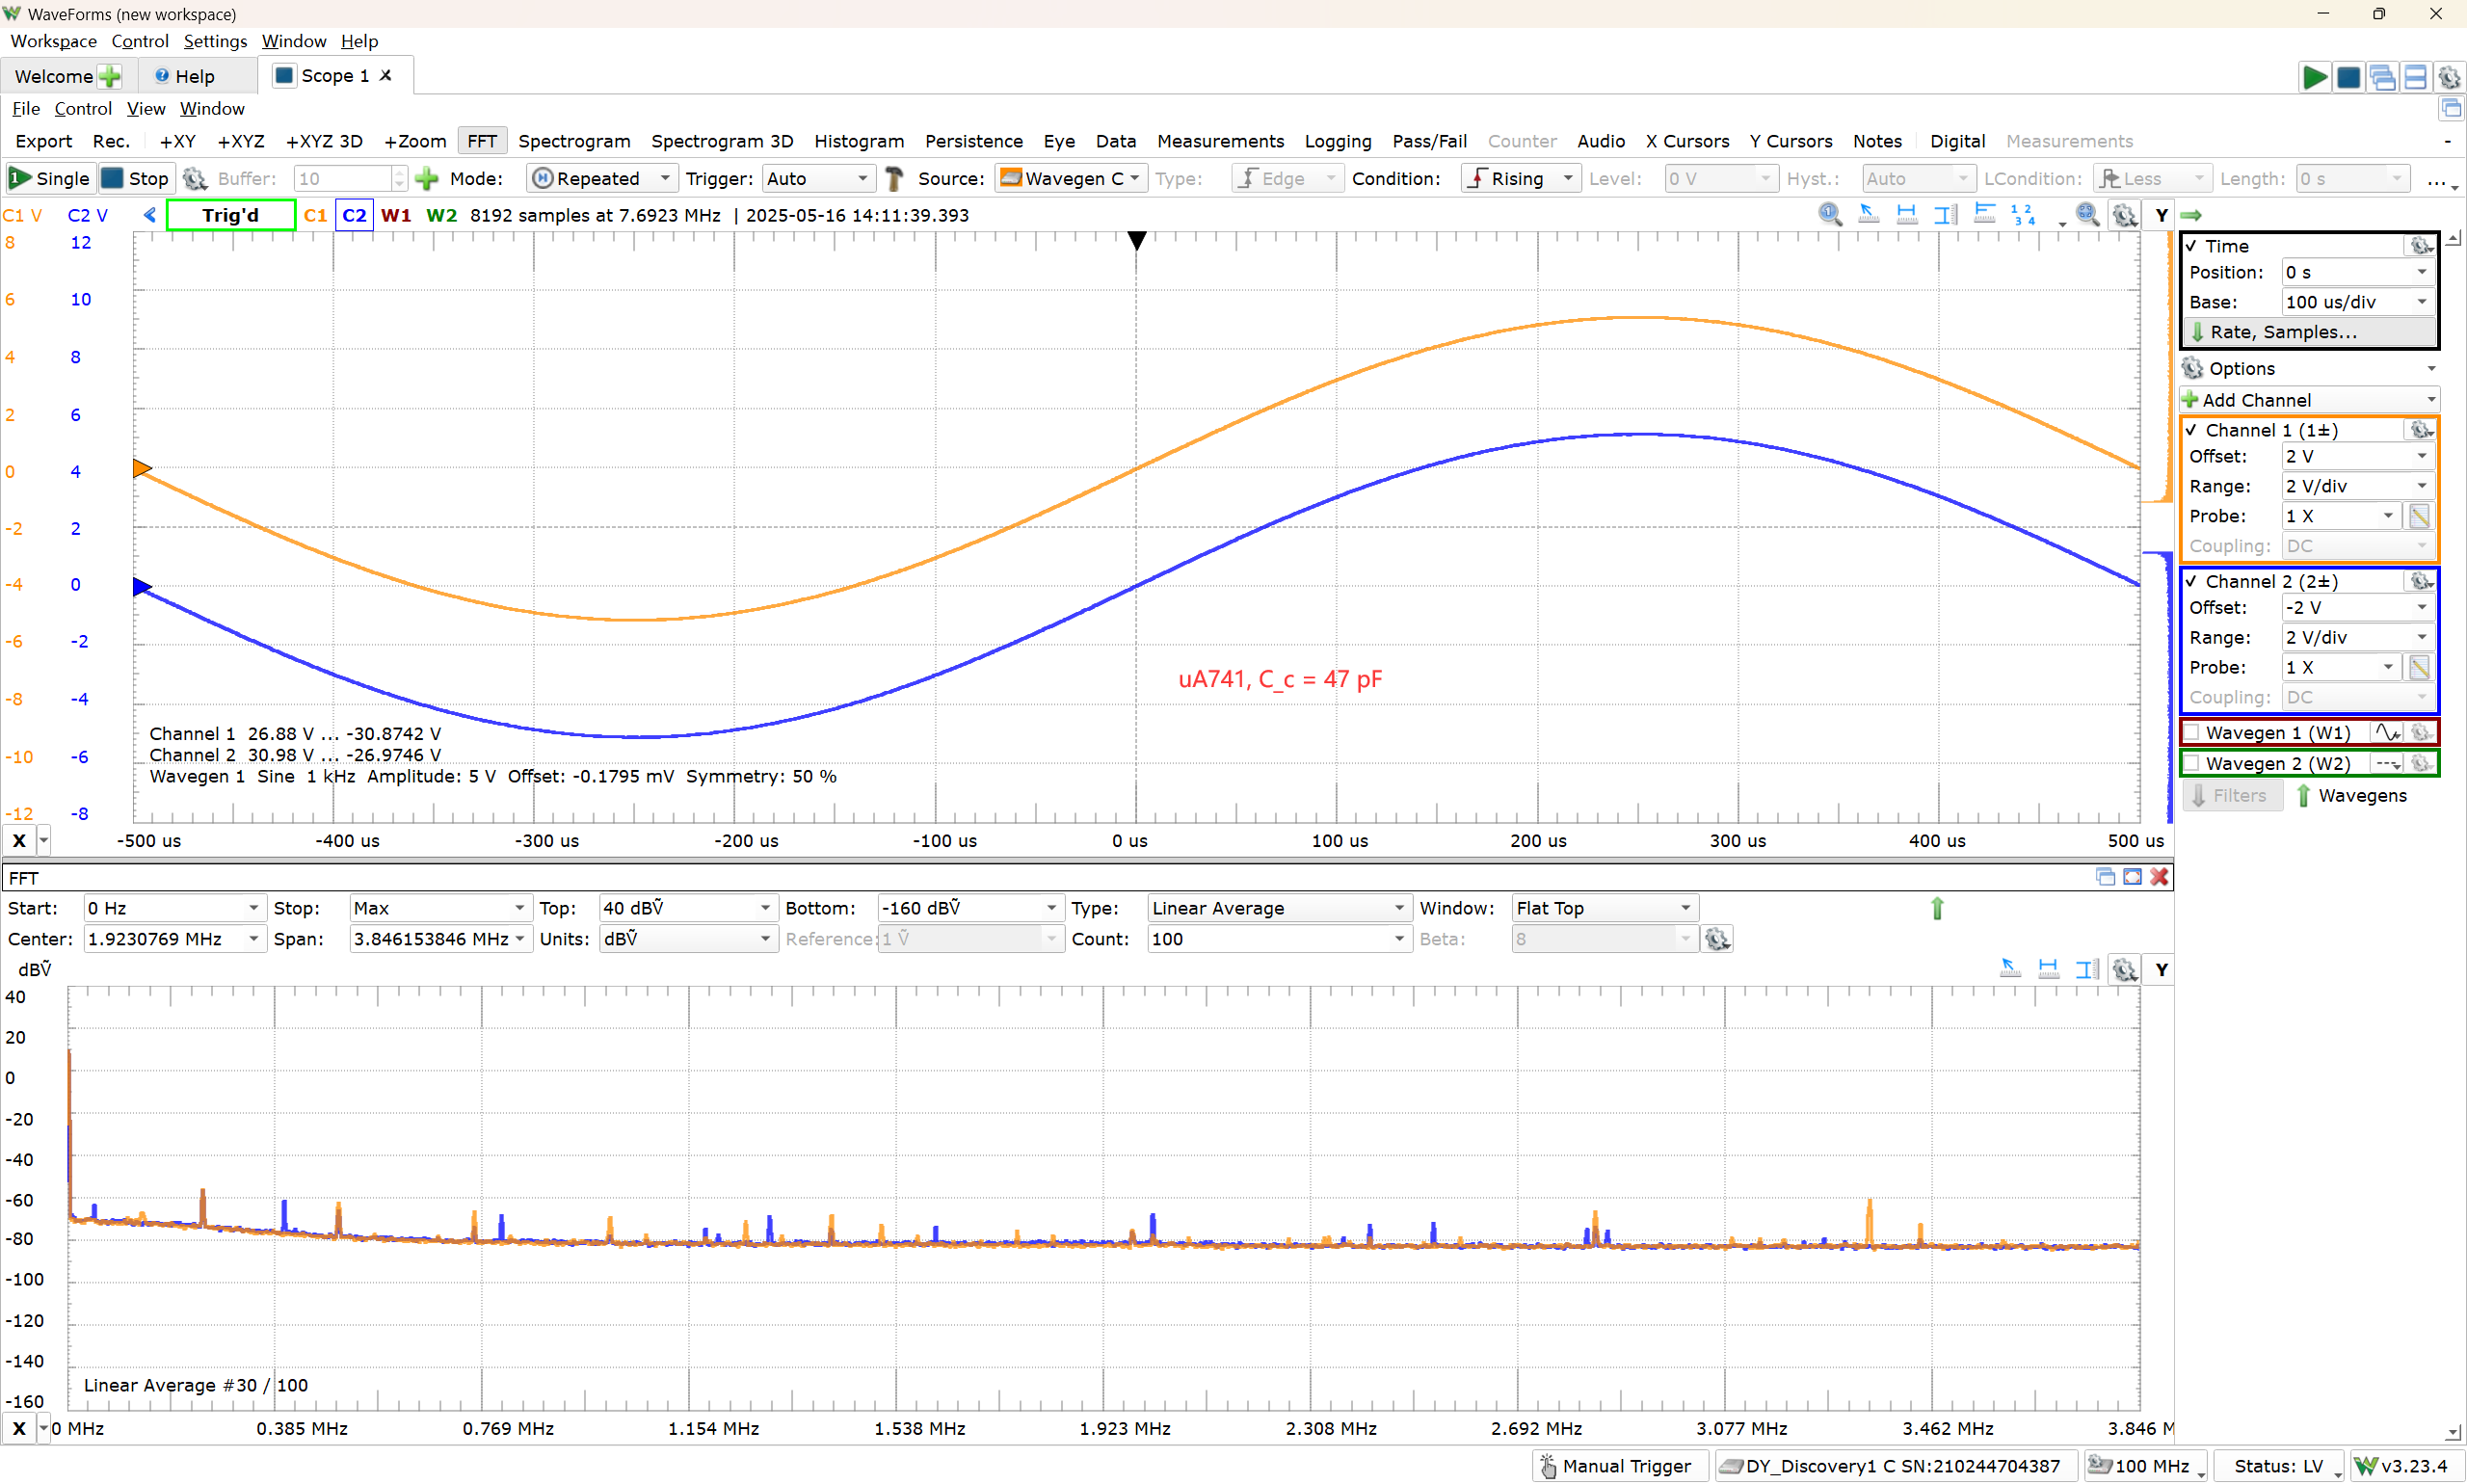
\includegraphics[width=\columnwidth]{LCE-06-07-运放设计/assets/uA741/test/unit buffer 2.png}
    \caption{uA741 unit buffer: sine input test; input 5 Vamp @ 1 kHz, CH1 (orange) input, CH2 (blue) output; misaligned display}
\end{figure}


\begin{figure}[H]\centering
    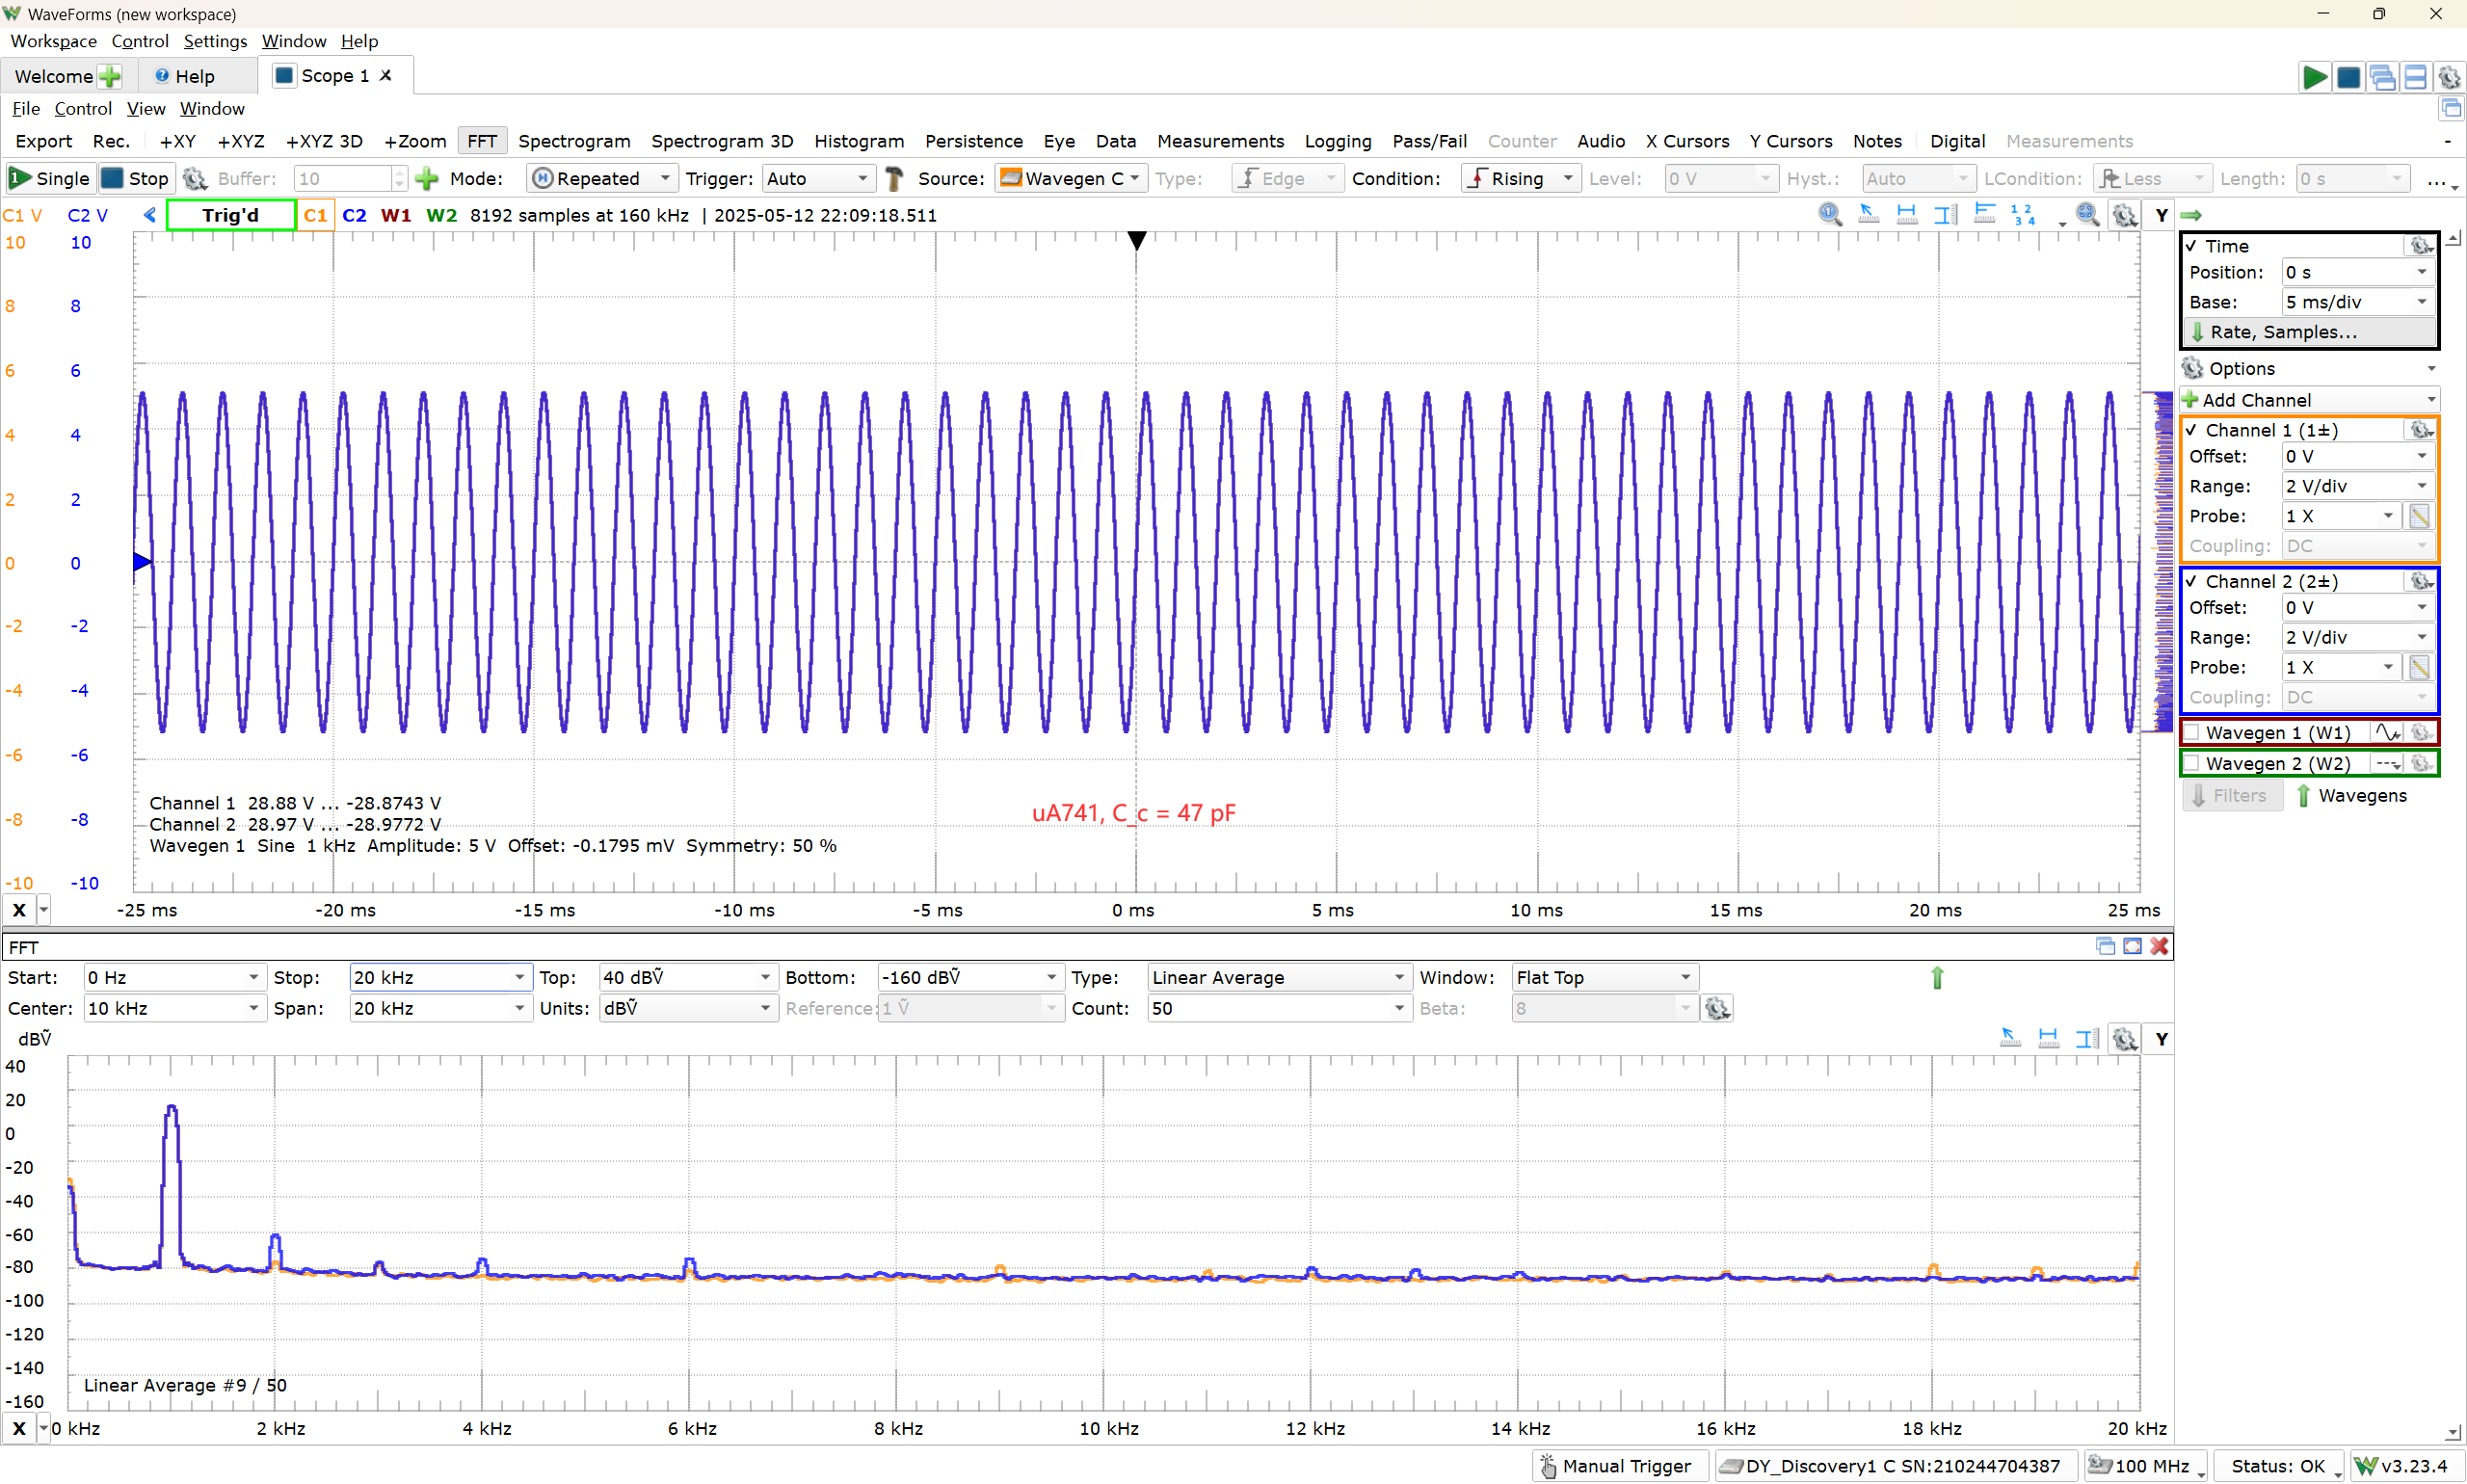
\includegraphics[width=\columnwidth]{LCE-06-07-运放设计/assets/uA741/test/unit buffer 3.png}
    \caption{uA741 unit buffer: harmonic distortion test; input 5 Vamp @ 1 kHz, CH1 (orange) input, CH2 (blue) output}
\end{figure}


\subsubsection{Inverting Amplifier}

\begin{figure}[H]\centering
    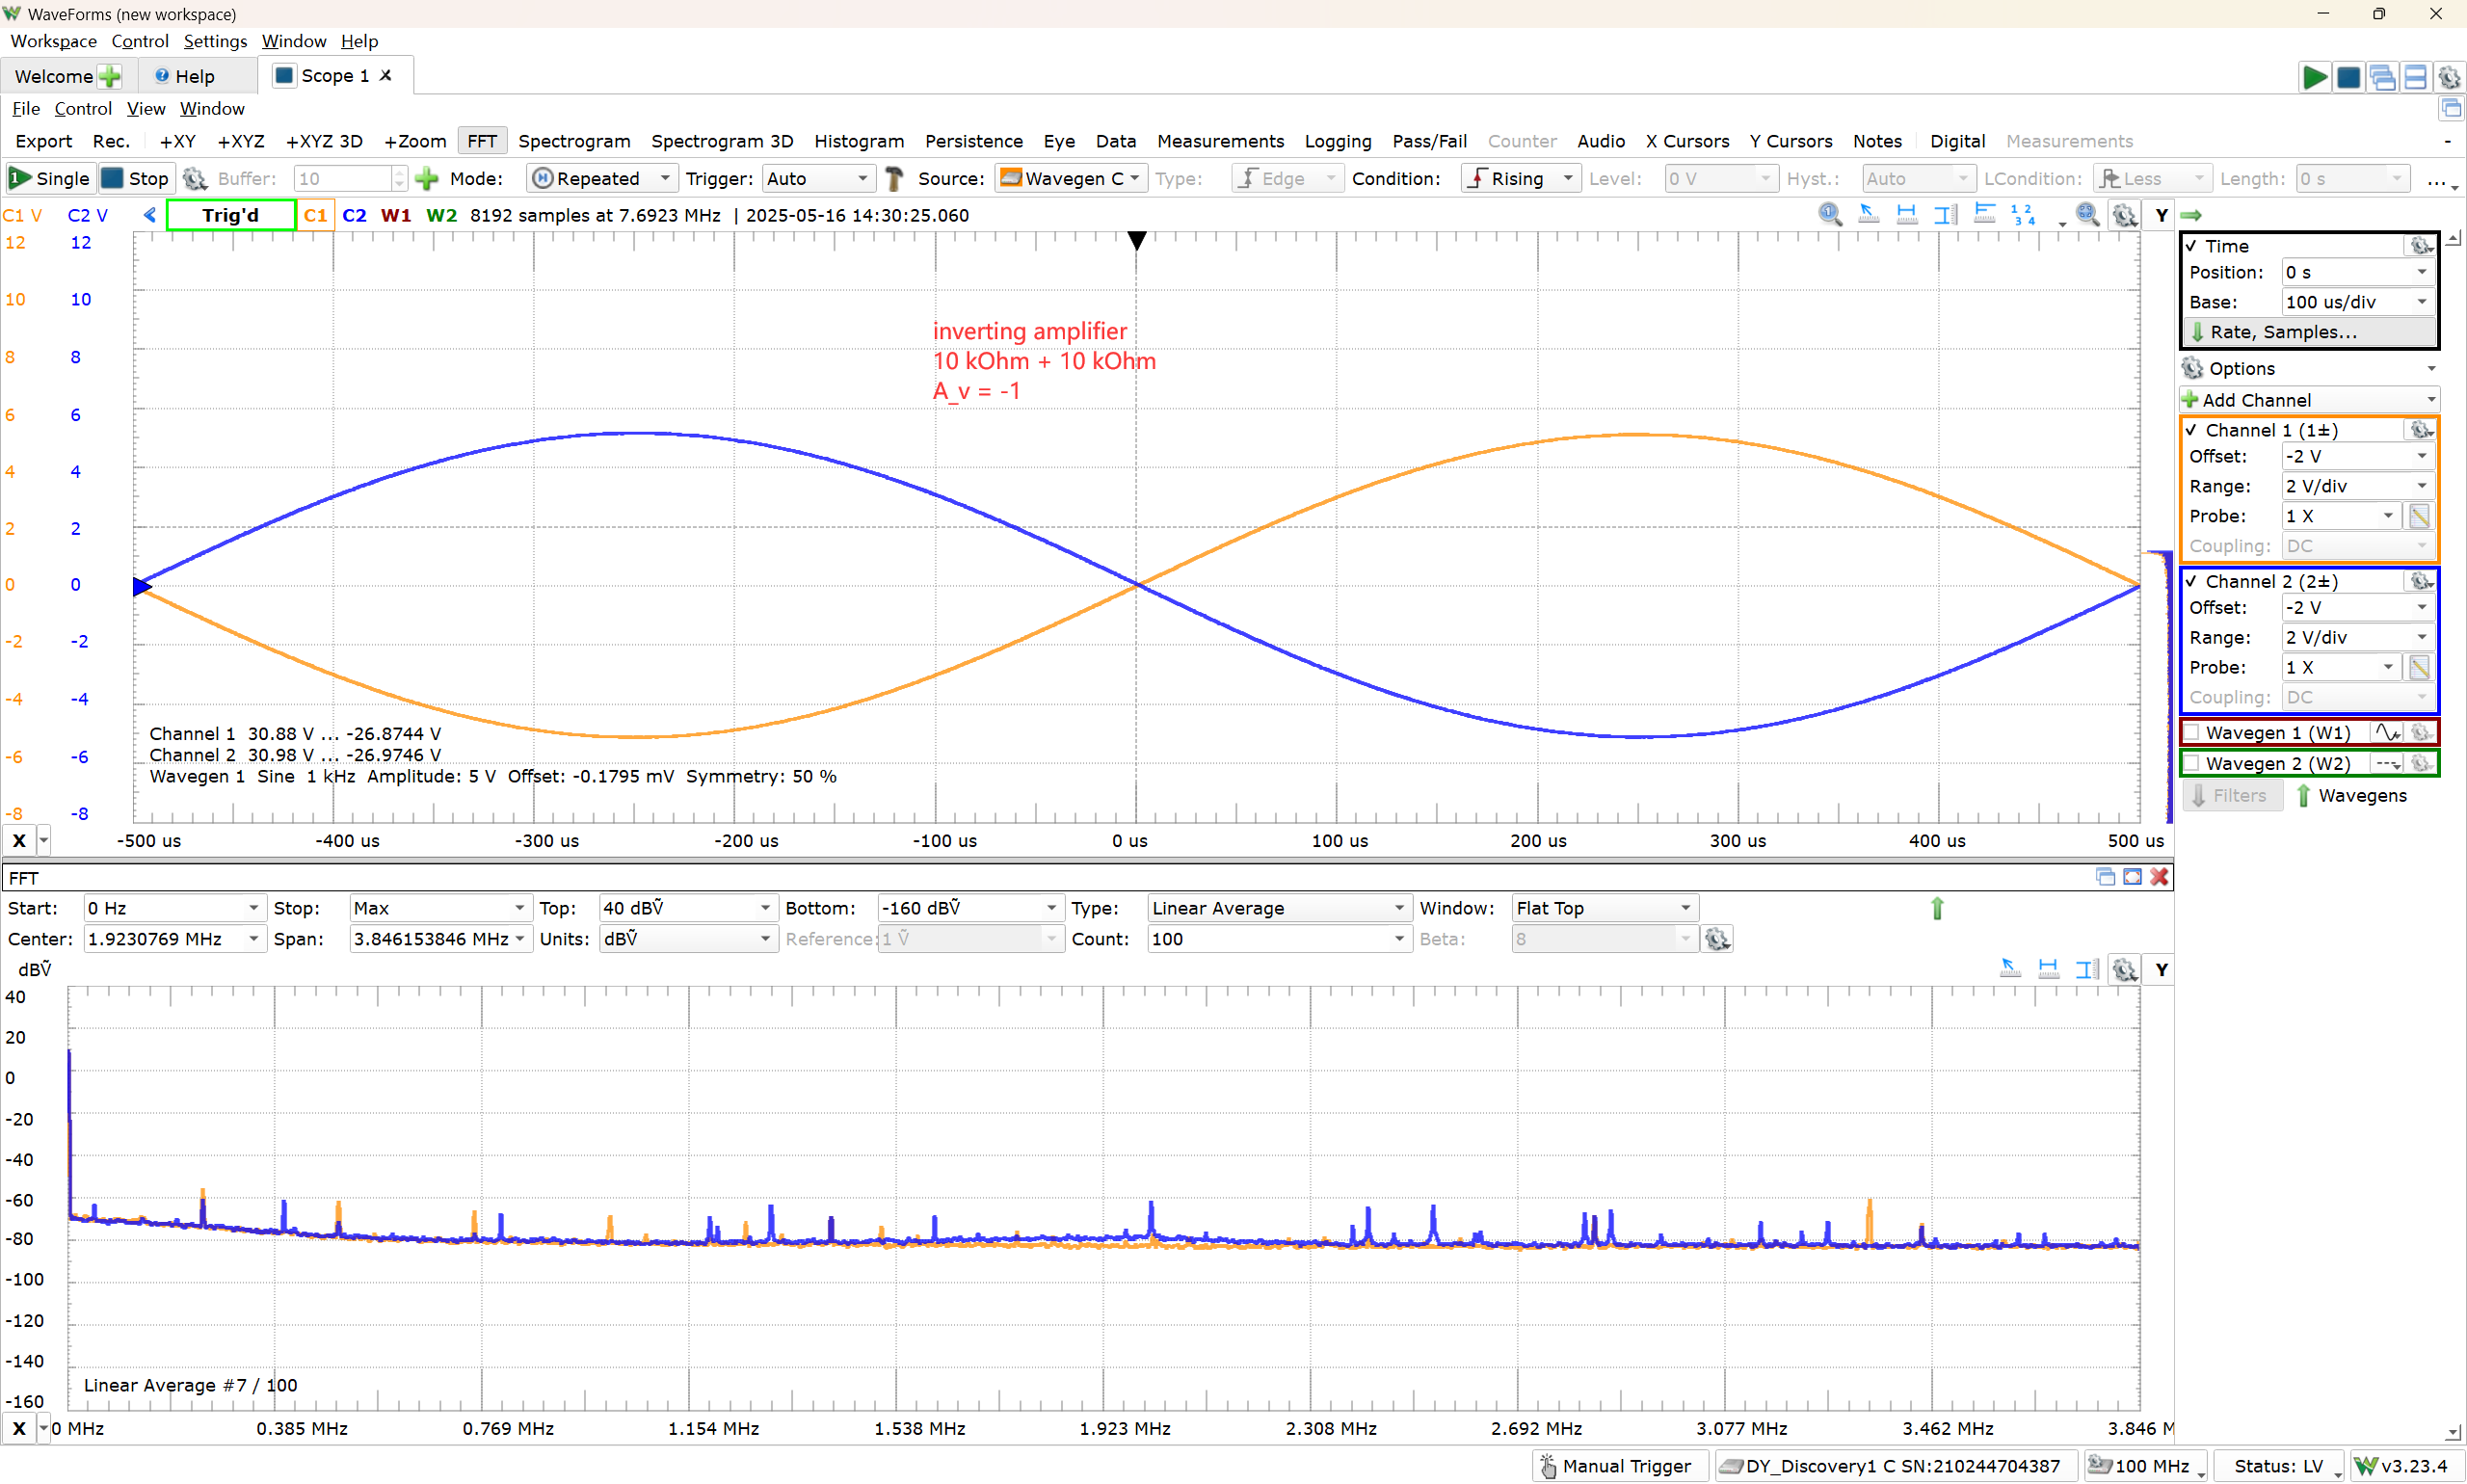
\includegraphics[width=\columnwidth]{LCE-06-07-运放设计/assets/uA741/test/inverting 1.png}
    \caption{uA741 inverting amplifier: sine input test; input 5 Vamp @ 1 kHz, CH1 (orange) input, CH2 (blue) output}
\end{figure}

\begin{figure}[H]\centering
    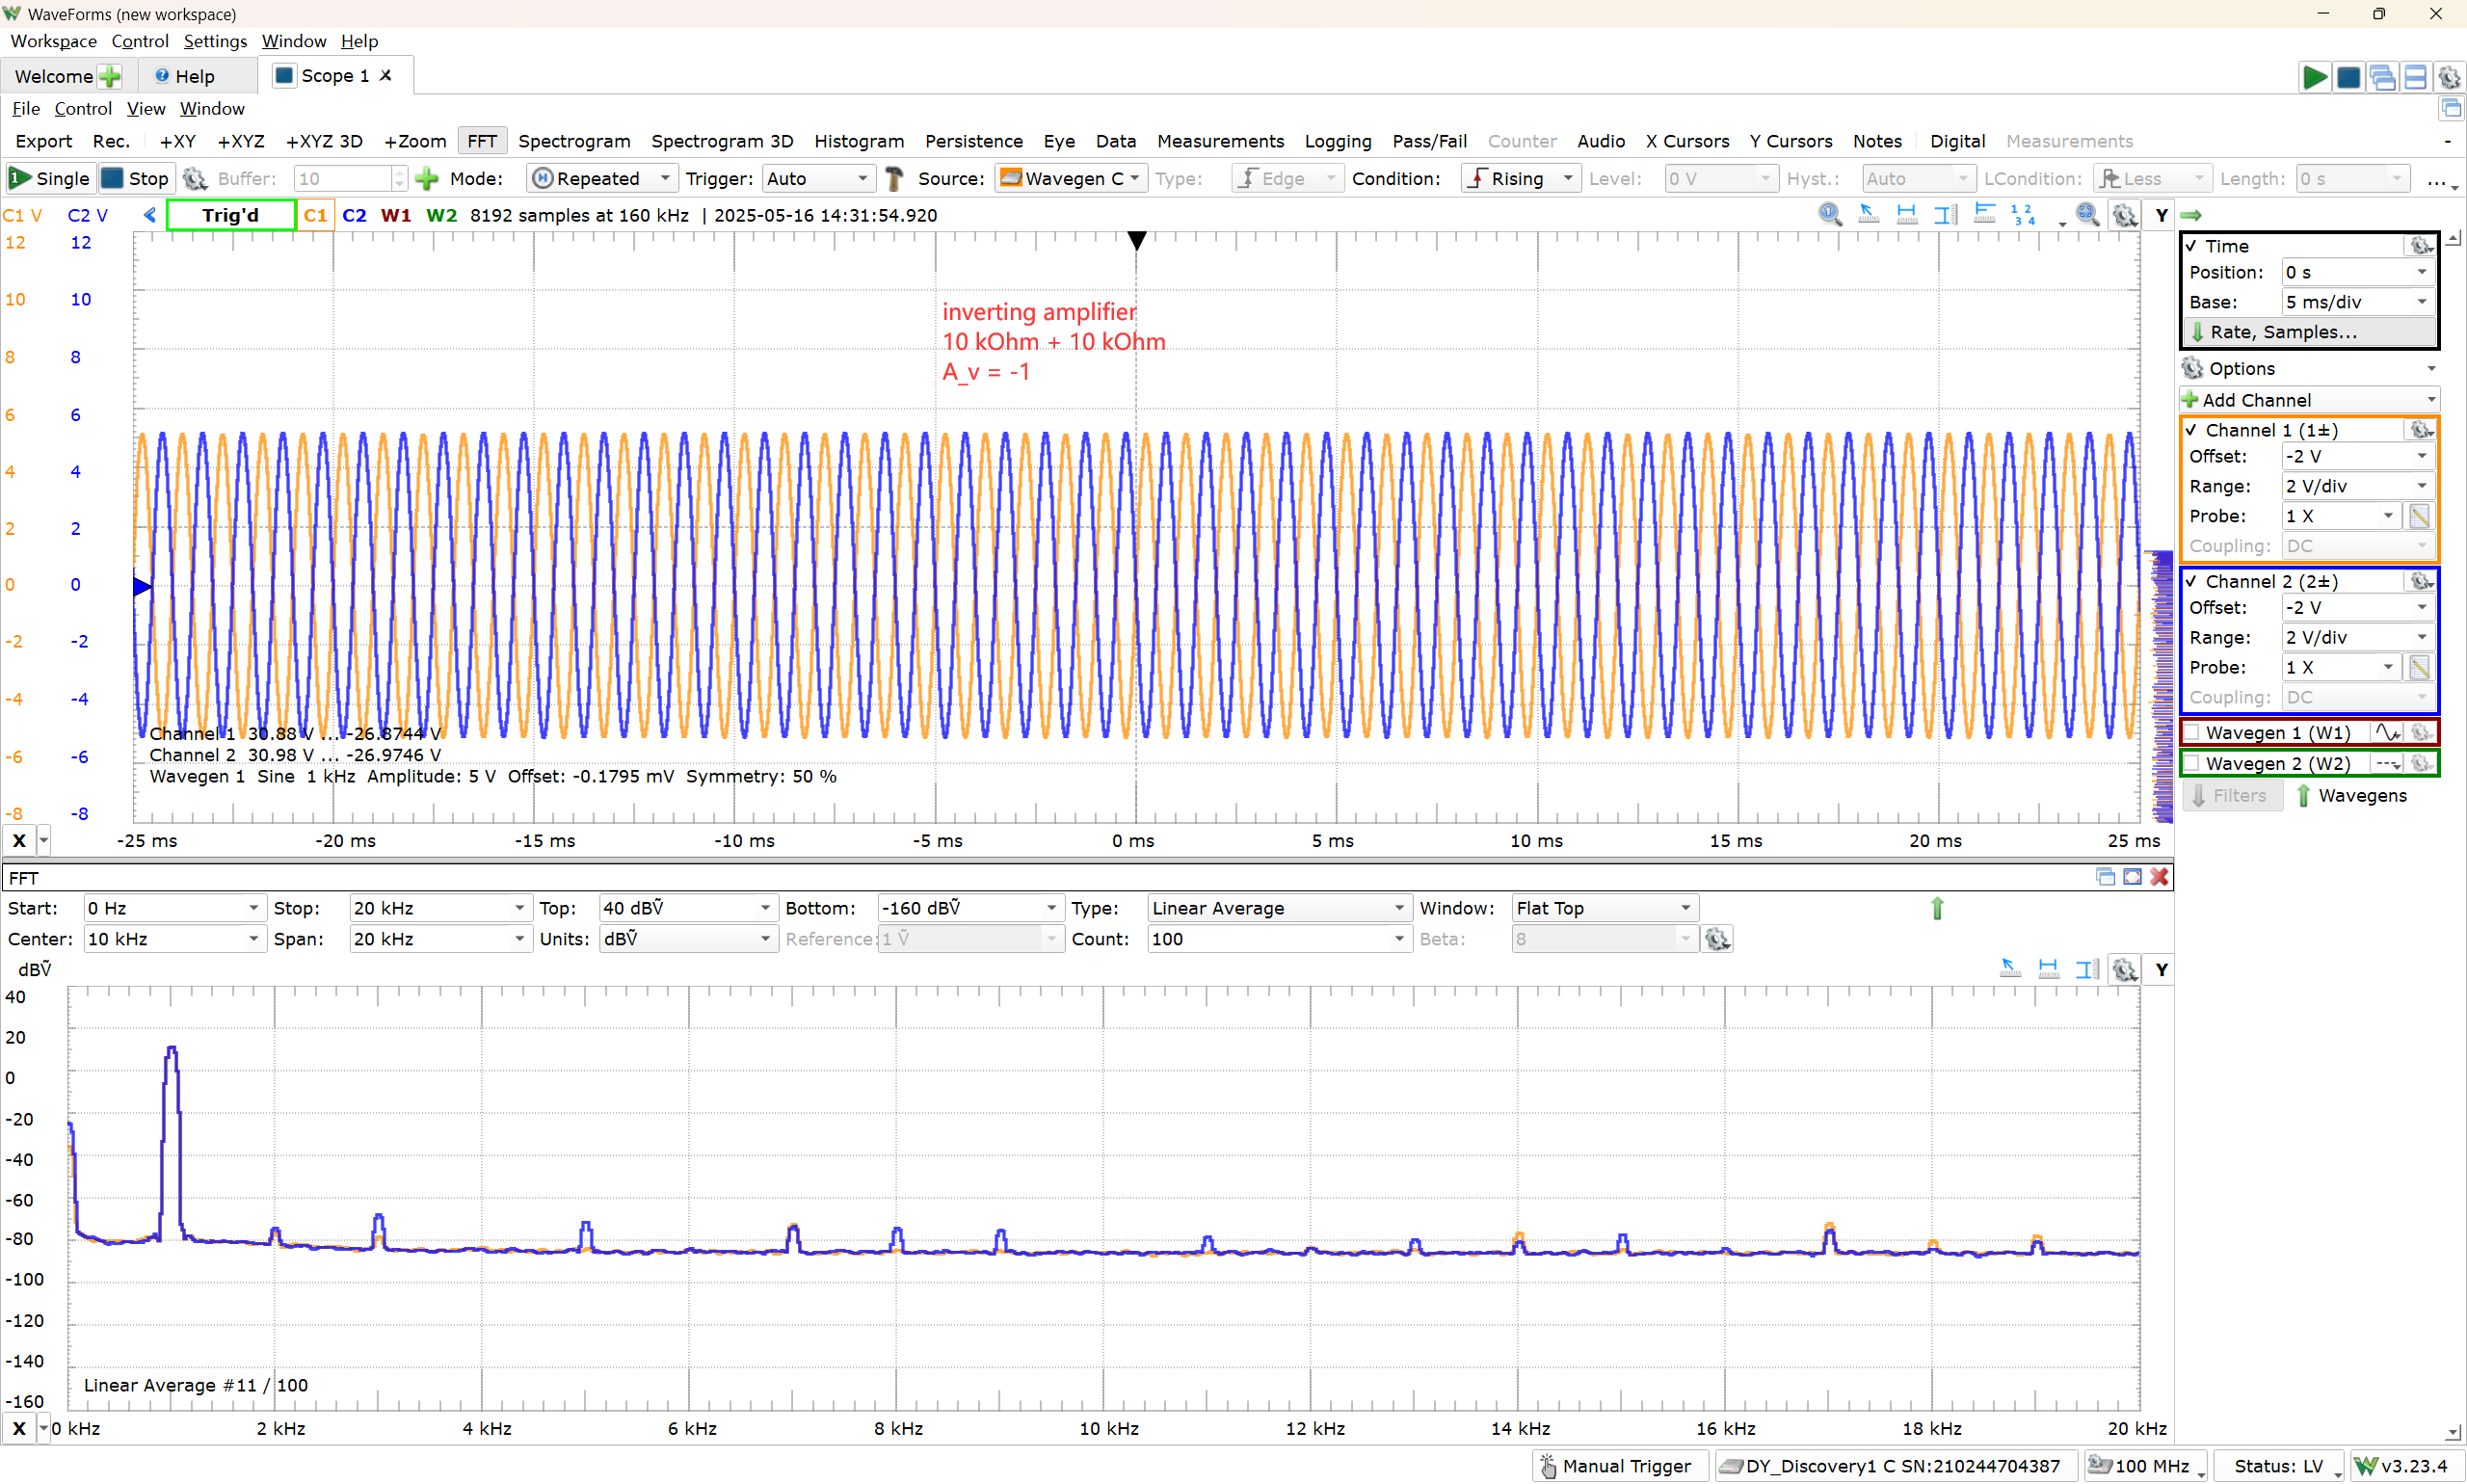
\includegraphics[width=\columnwidth]{LCE-06-07-运放设计/assets/uA741/test/inverting 2.png}
    \caption{uA741 inverting amplifier: harmonic distortion test; input 5 Vamp @ 1 kHz, CH1 (orange) input, CH2 (blue) output}
\end{figure}

\begin{figure}[H]\centering
    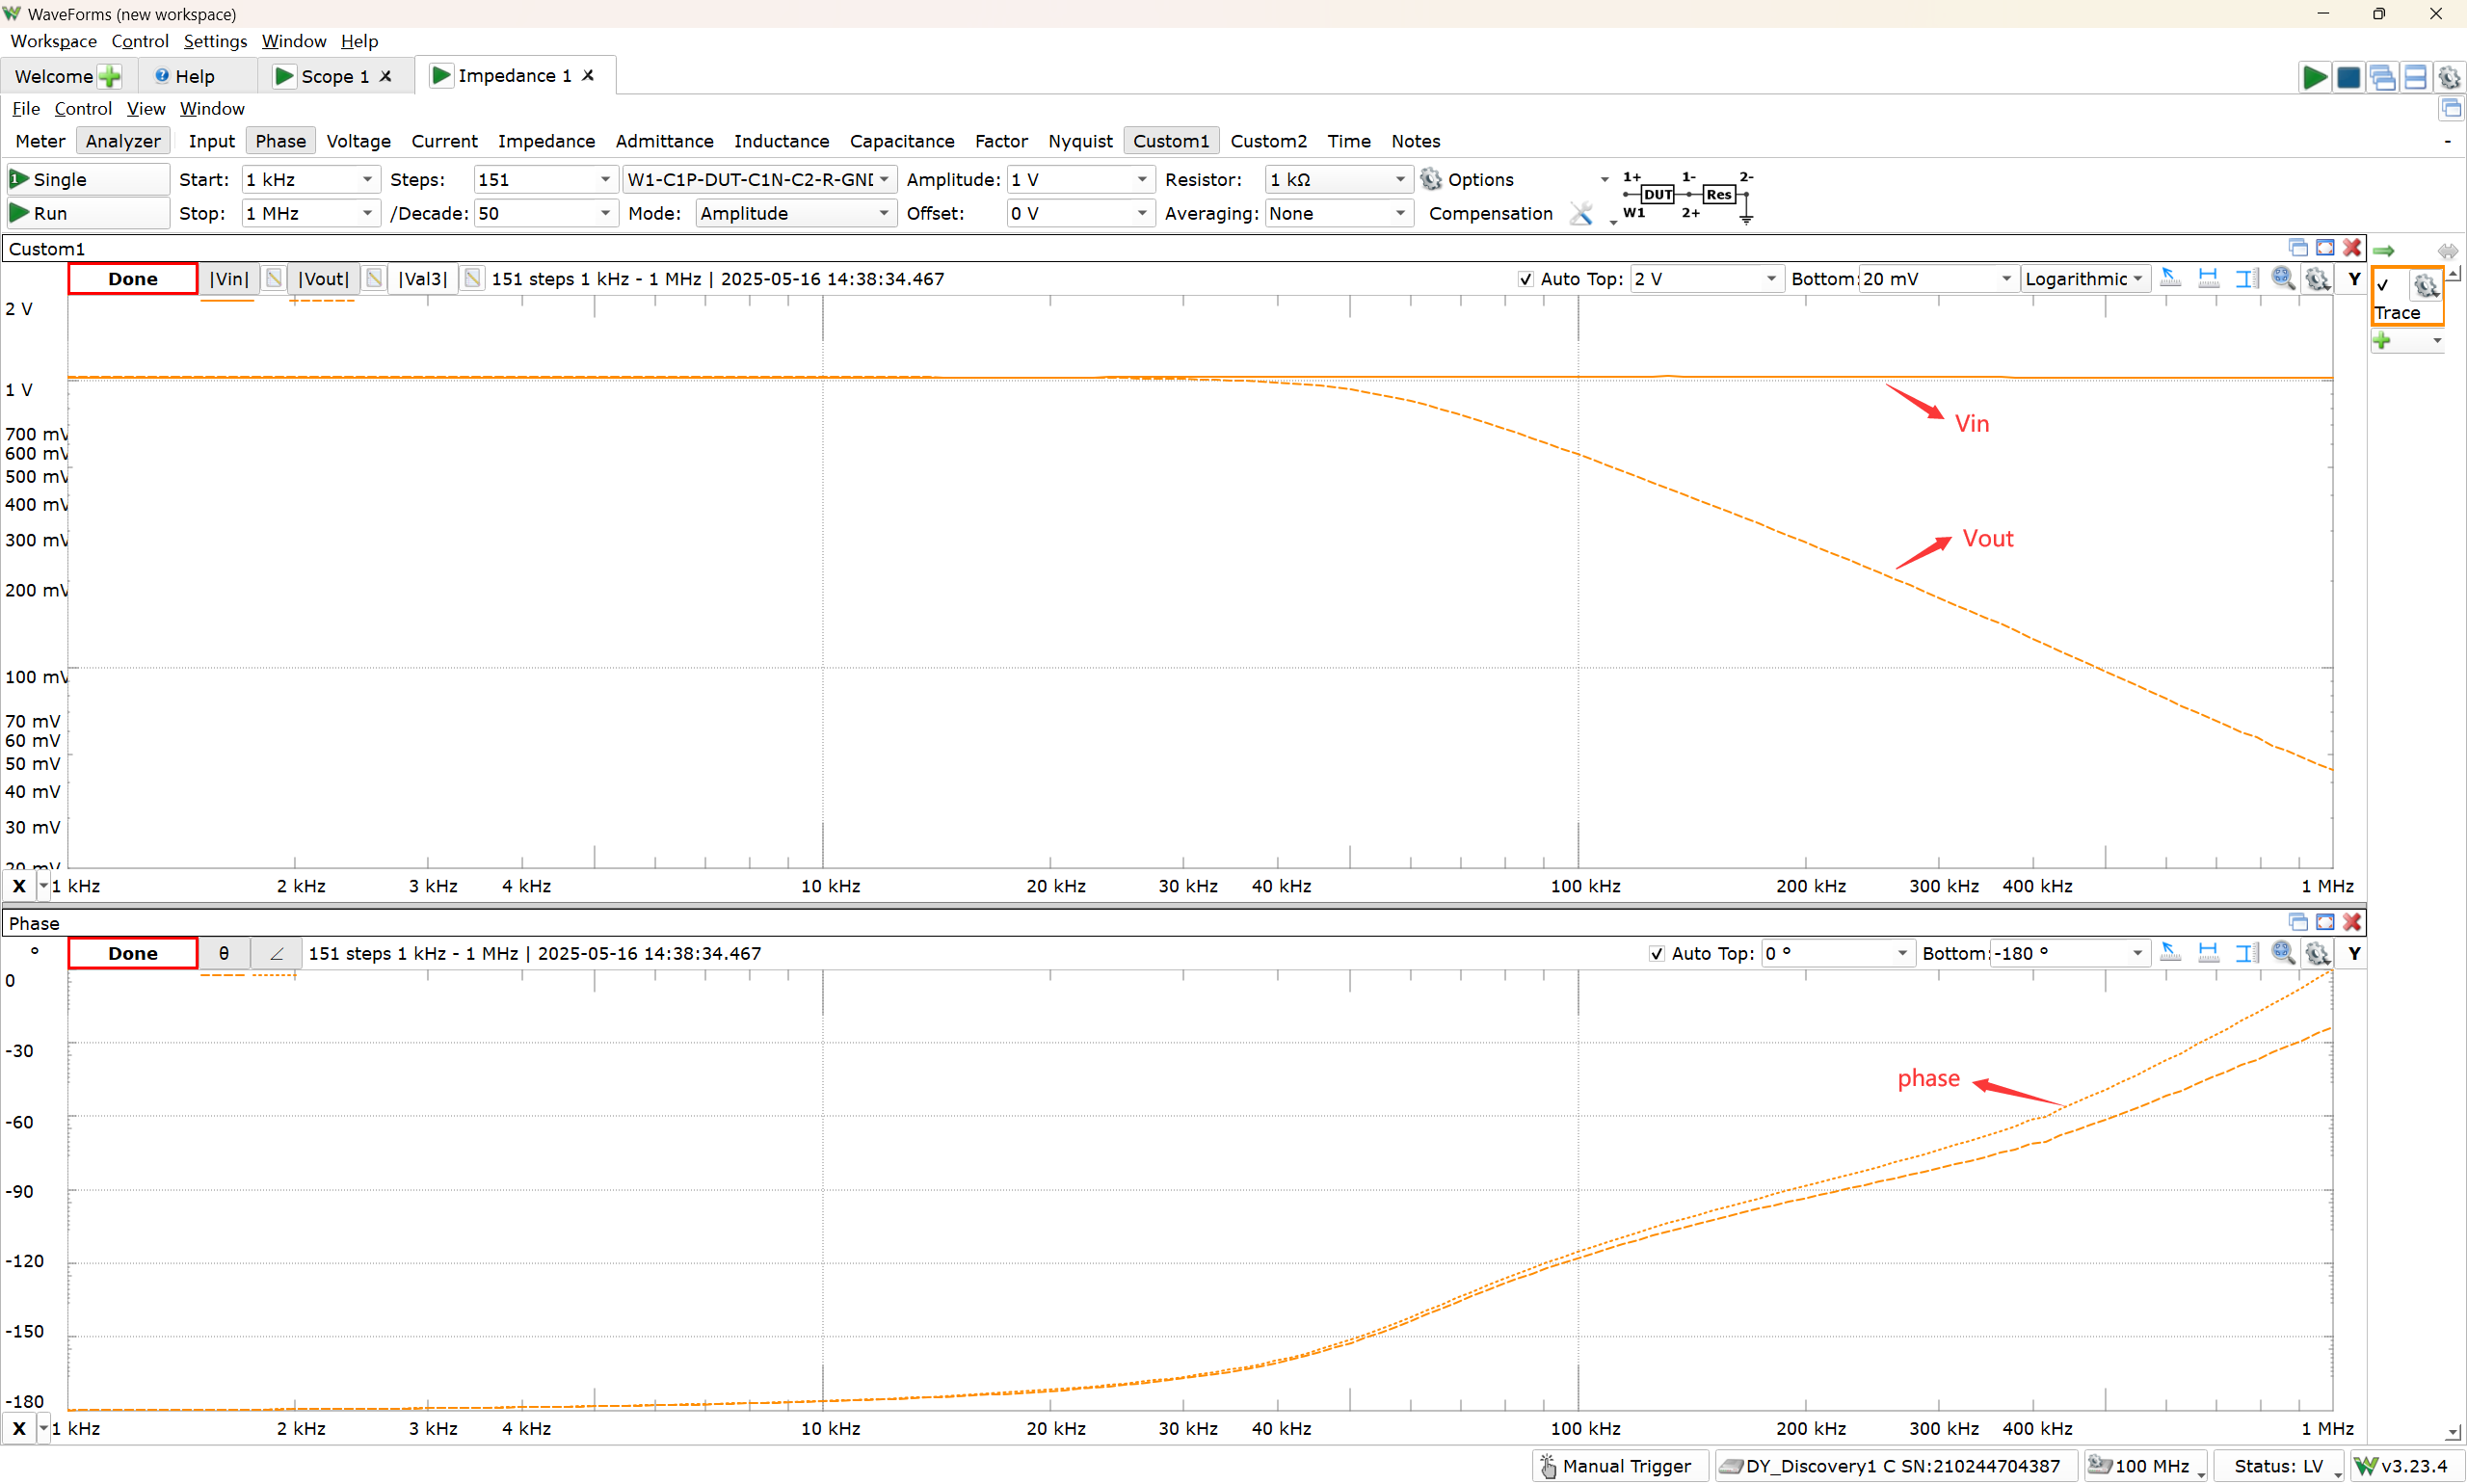
\includegraphics[width=\columnwidth]{LCE-06-07-运放设计/assets/uA741/test/inverting 3.png}
    \caption{uA741 inverting amplifier: frequency response; input 1 Vamp from 1 kHz to 100 kHz, CH1 (orange) input, CH2 (blue) output}
\end{figure}

\subsubsection{Integrating Circuit}

\begin{figure}[H]\centering
    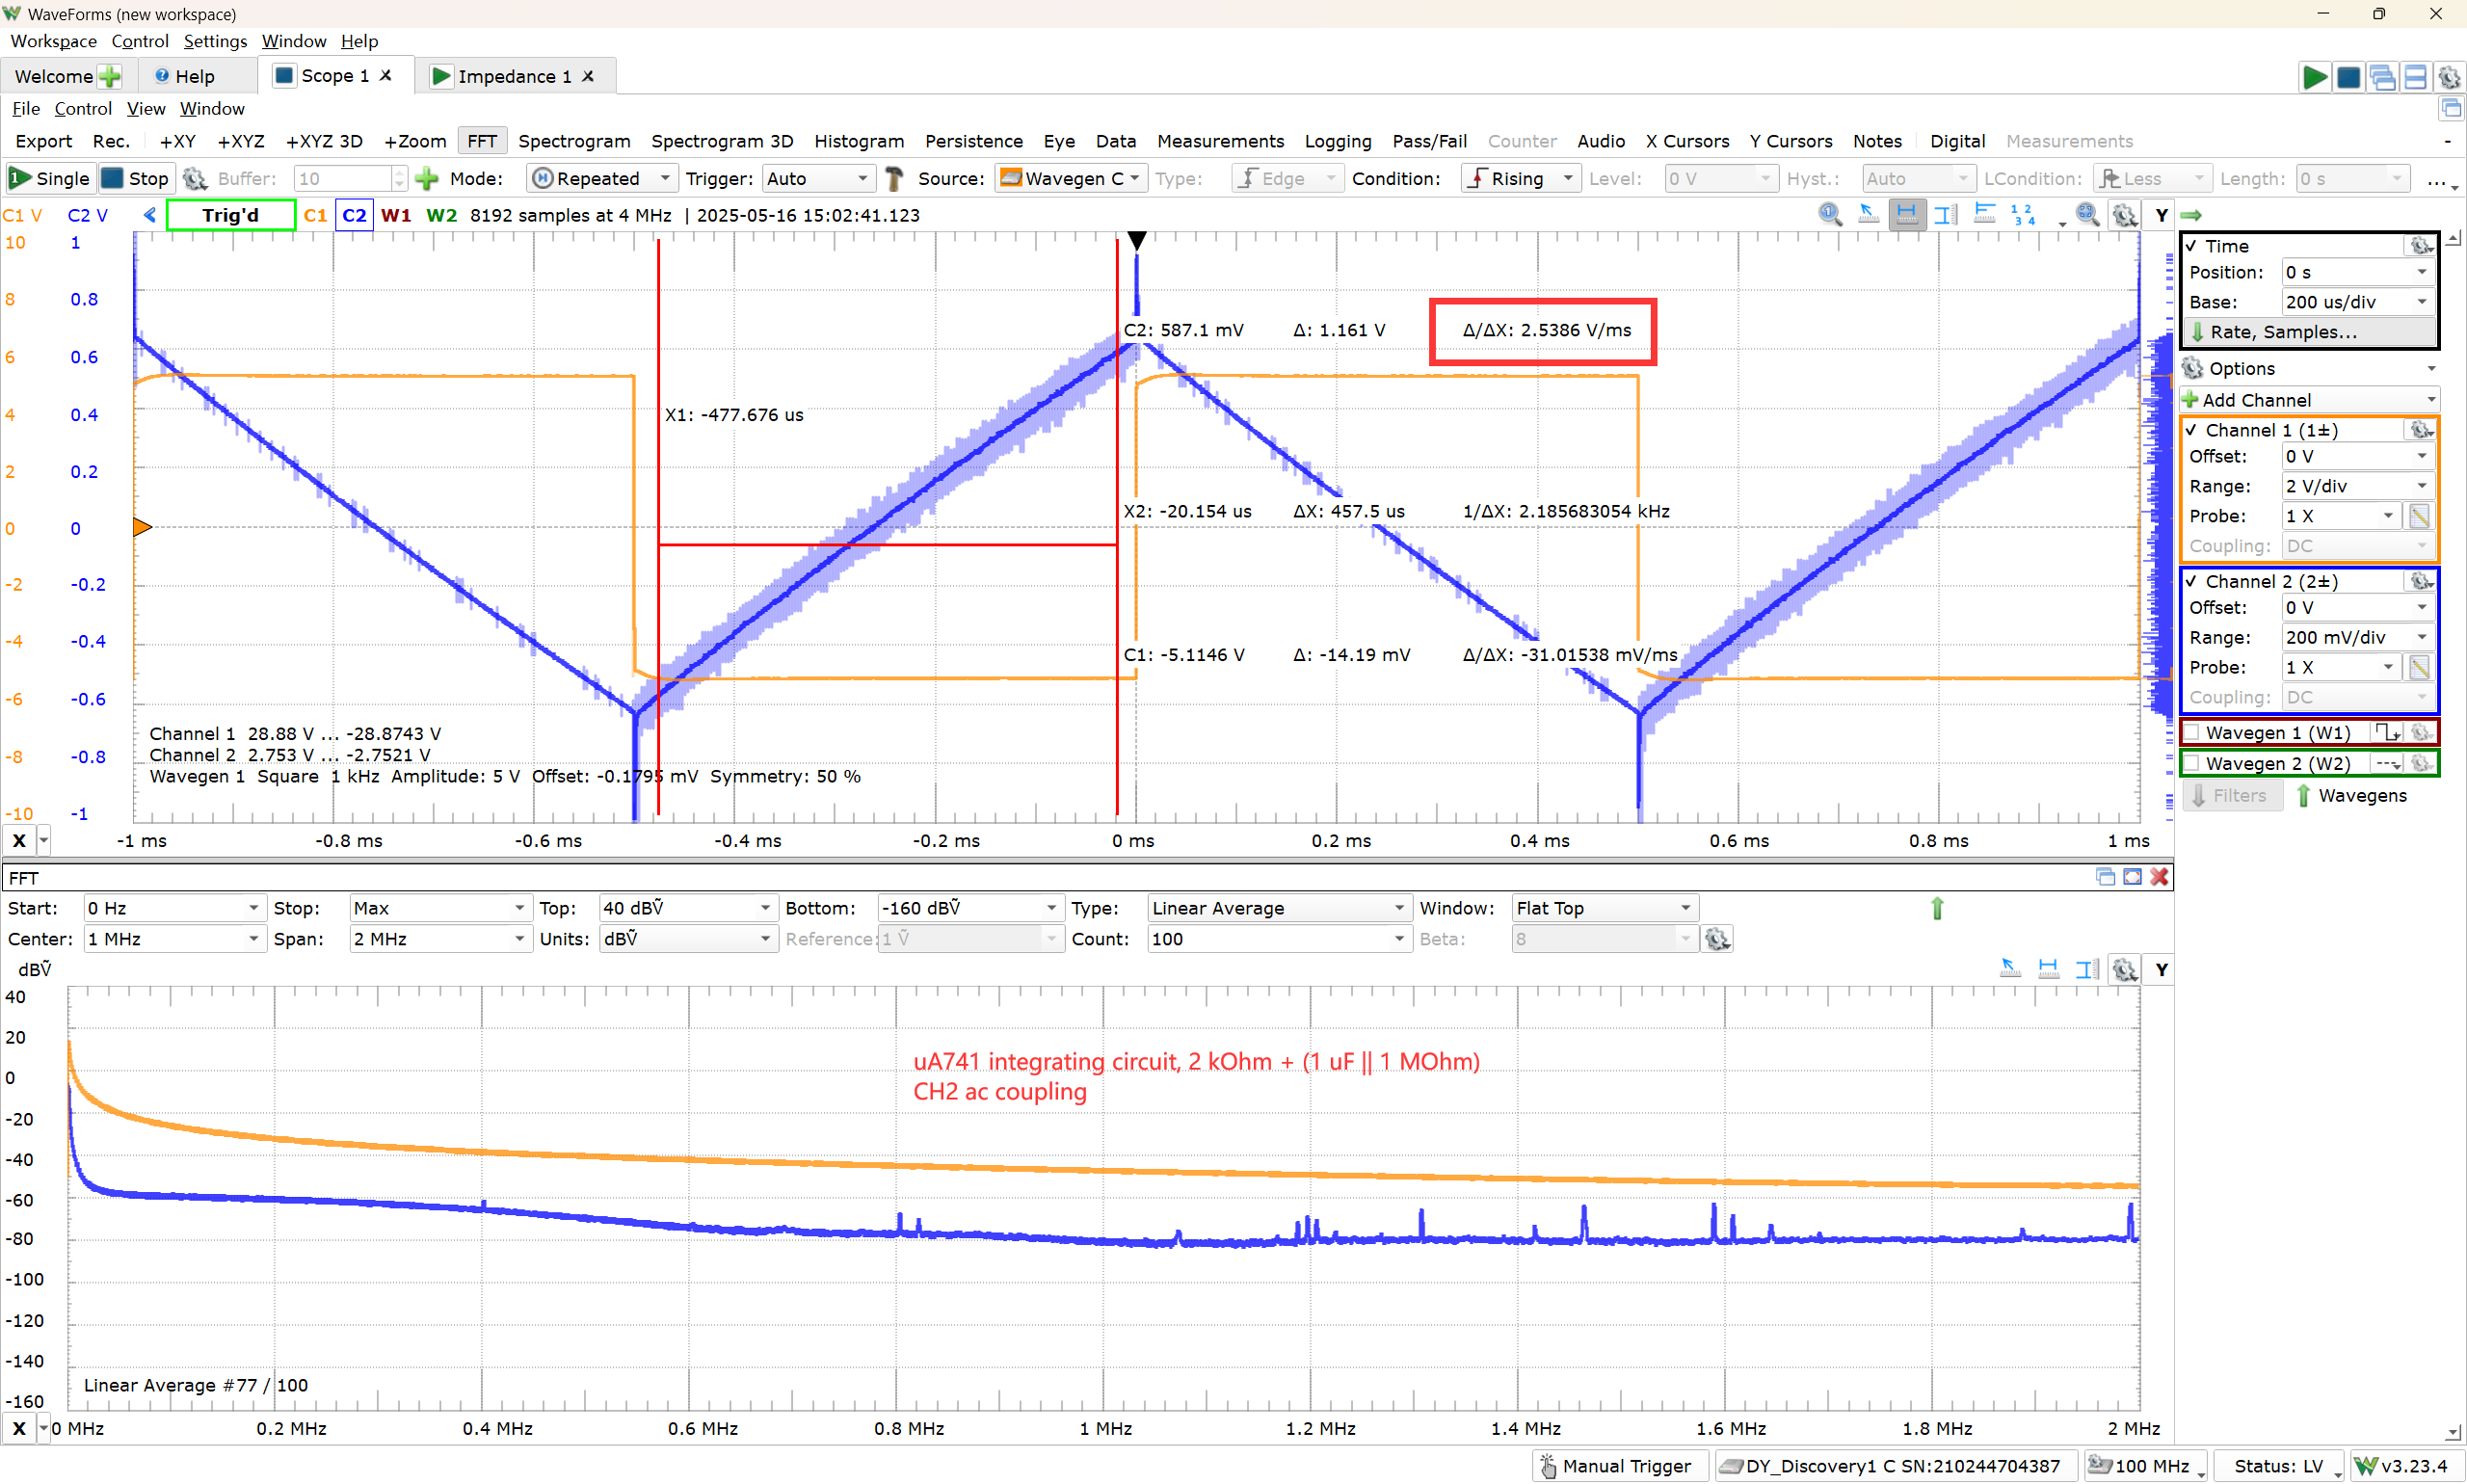
\includegraphics[width=\columnwidth]{LCE-06-07-运放设计/assets/uA741/test/integrating 1.png}
    \caption{uA741 integrating circuit: square input; input 5 Vamp @ 1 kHz, CH1 (orange) input, CH2 (blue) output}
\end{figure}

\subsubsection{Square Wave Generator}

\begin{figure}[H]\centering
    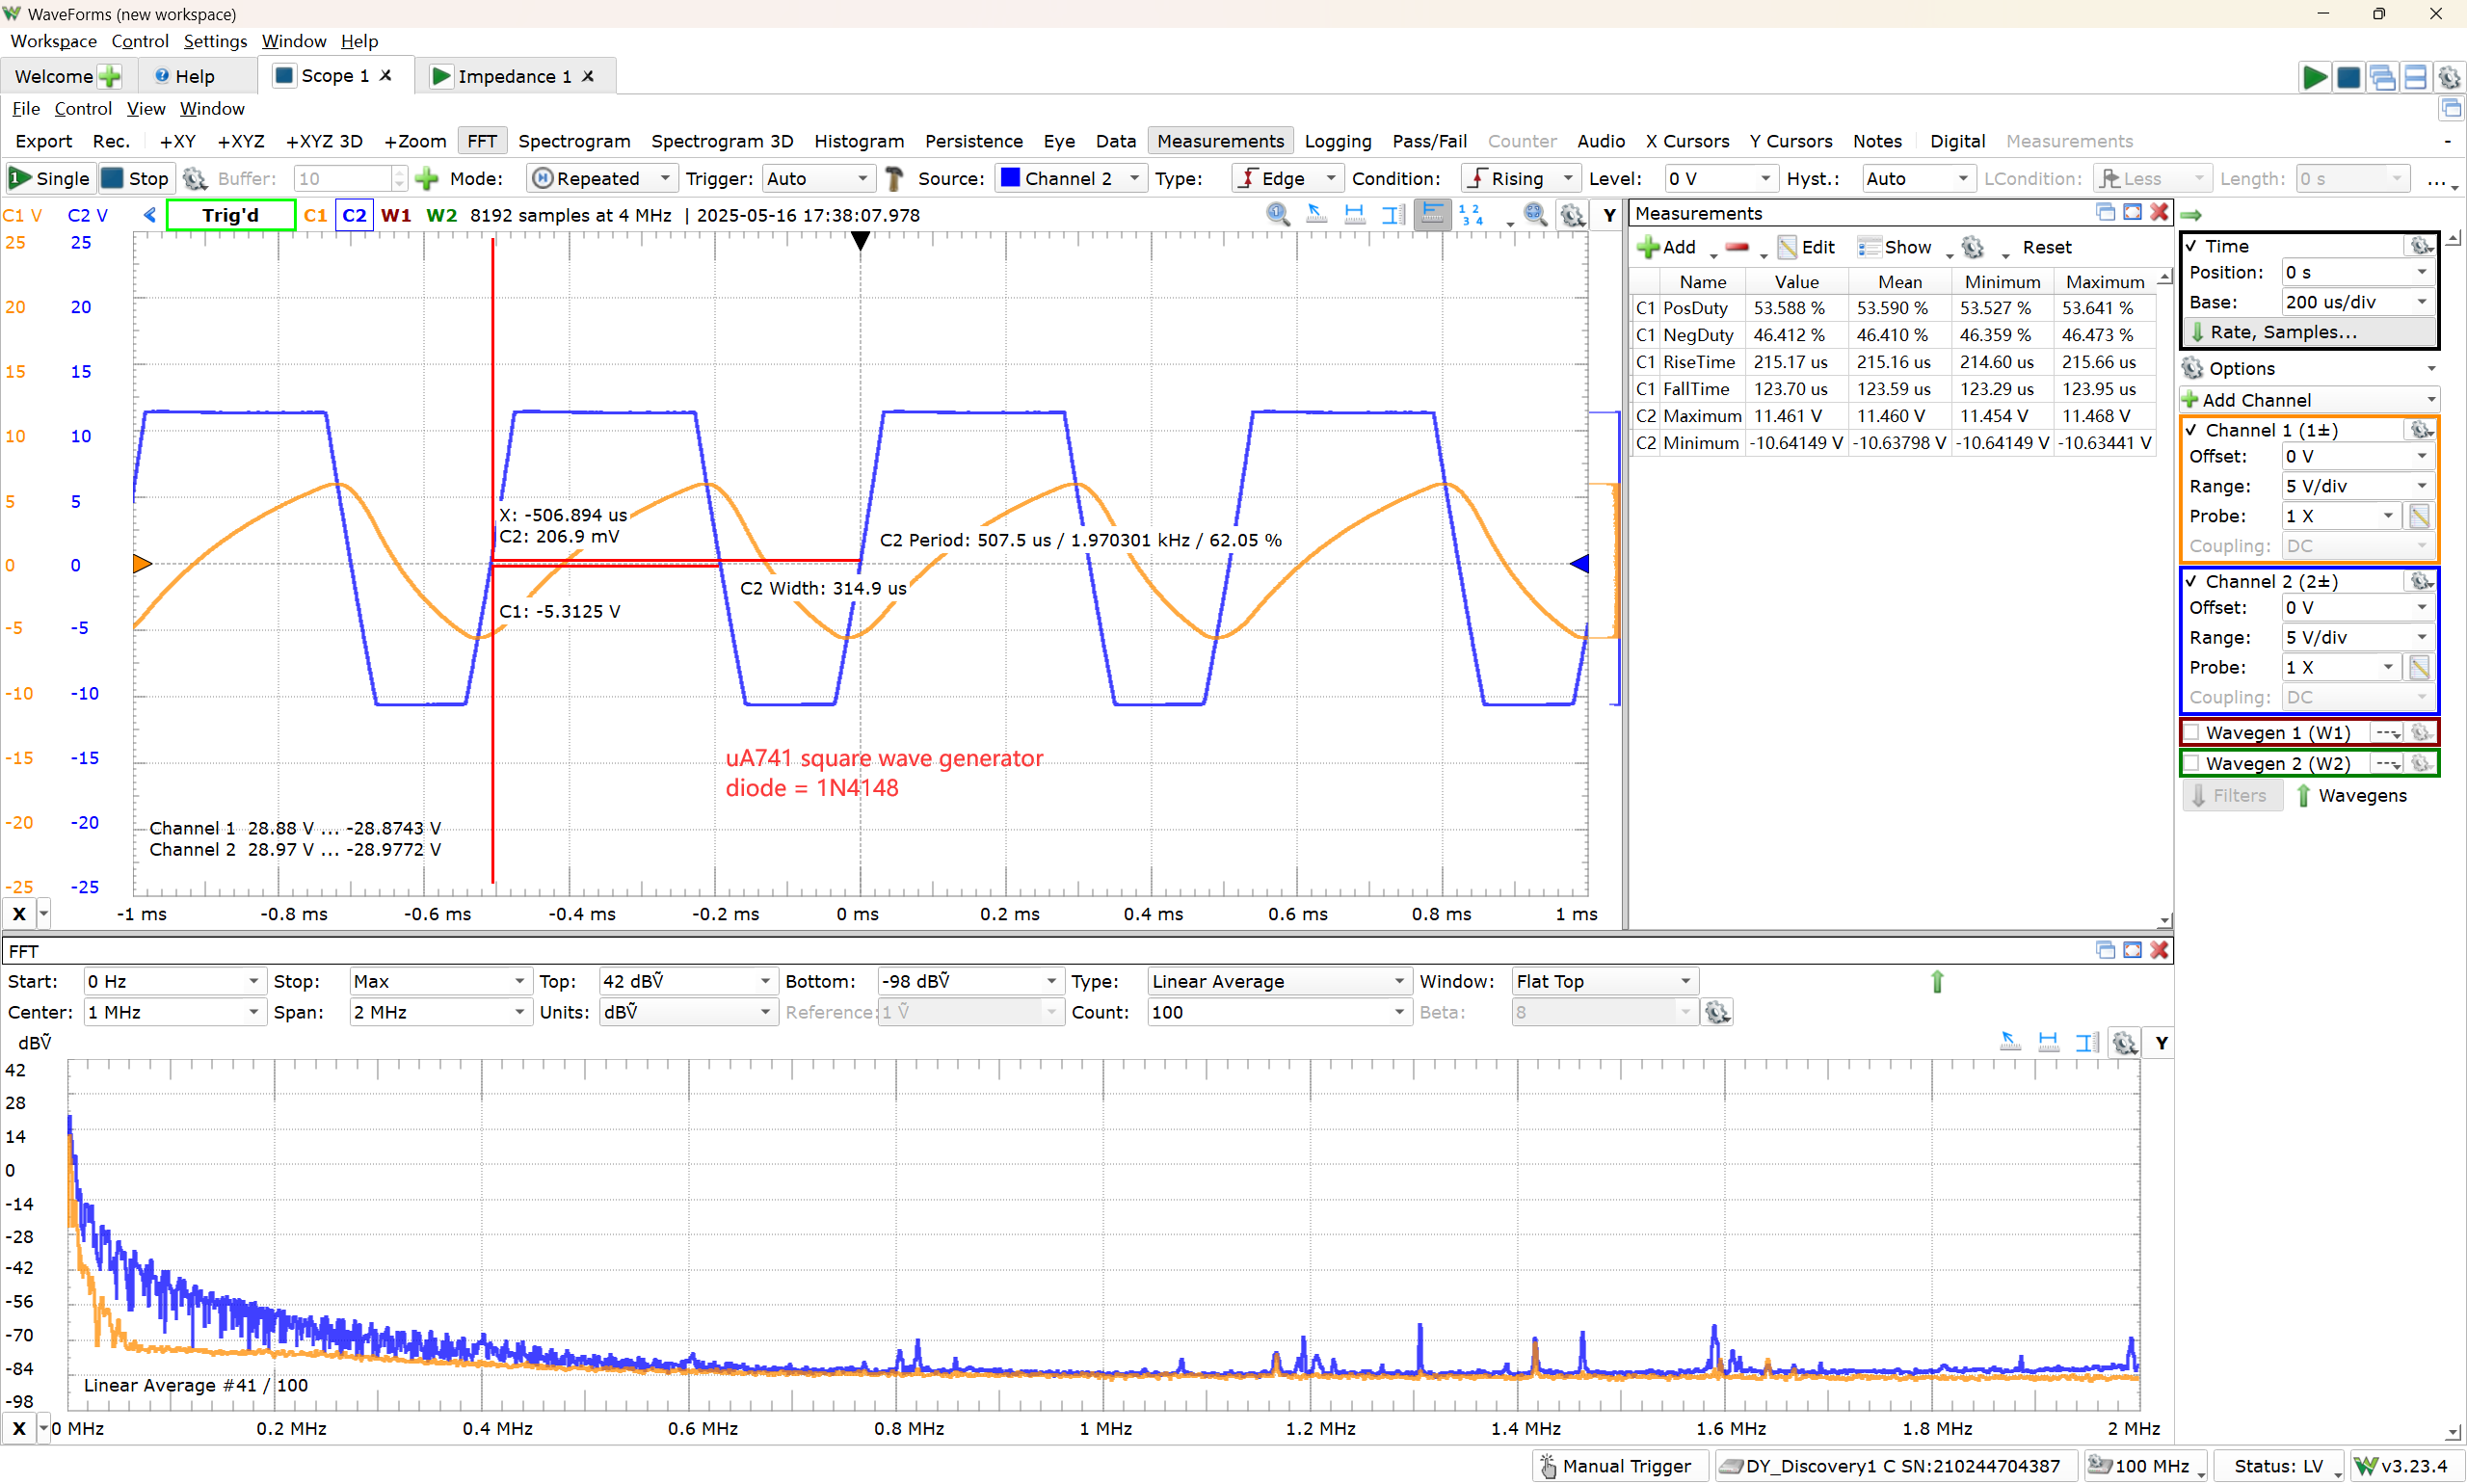
\includegraphics[width=\columnwidth]{LCE-06-07-运放设计/assets/uA741/test/square.png}
    \caption{uA741 square wave generator: CH2 (blue) output}
\end{figure}

\subsubsection{Wien-Bridge Oscillator}

\begin{figure}[H]\centering
    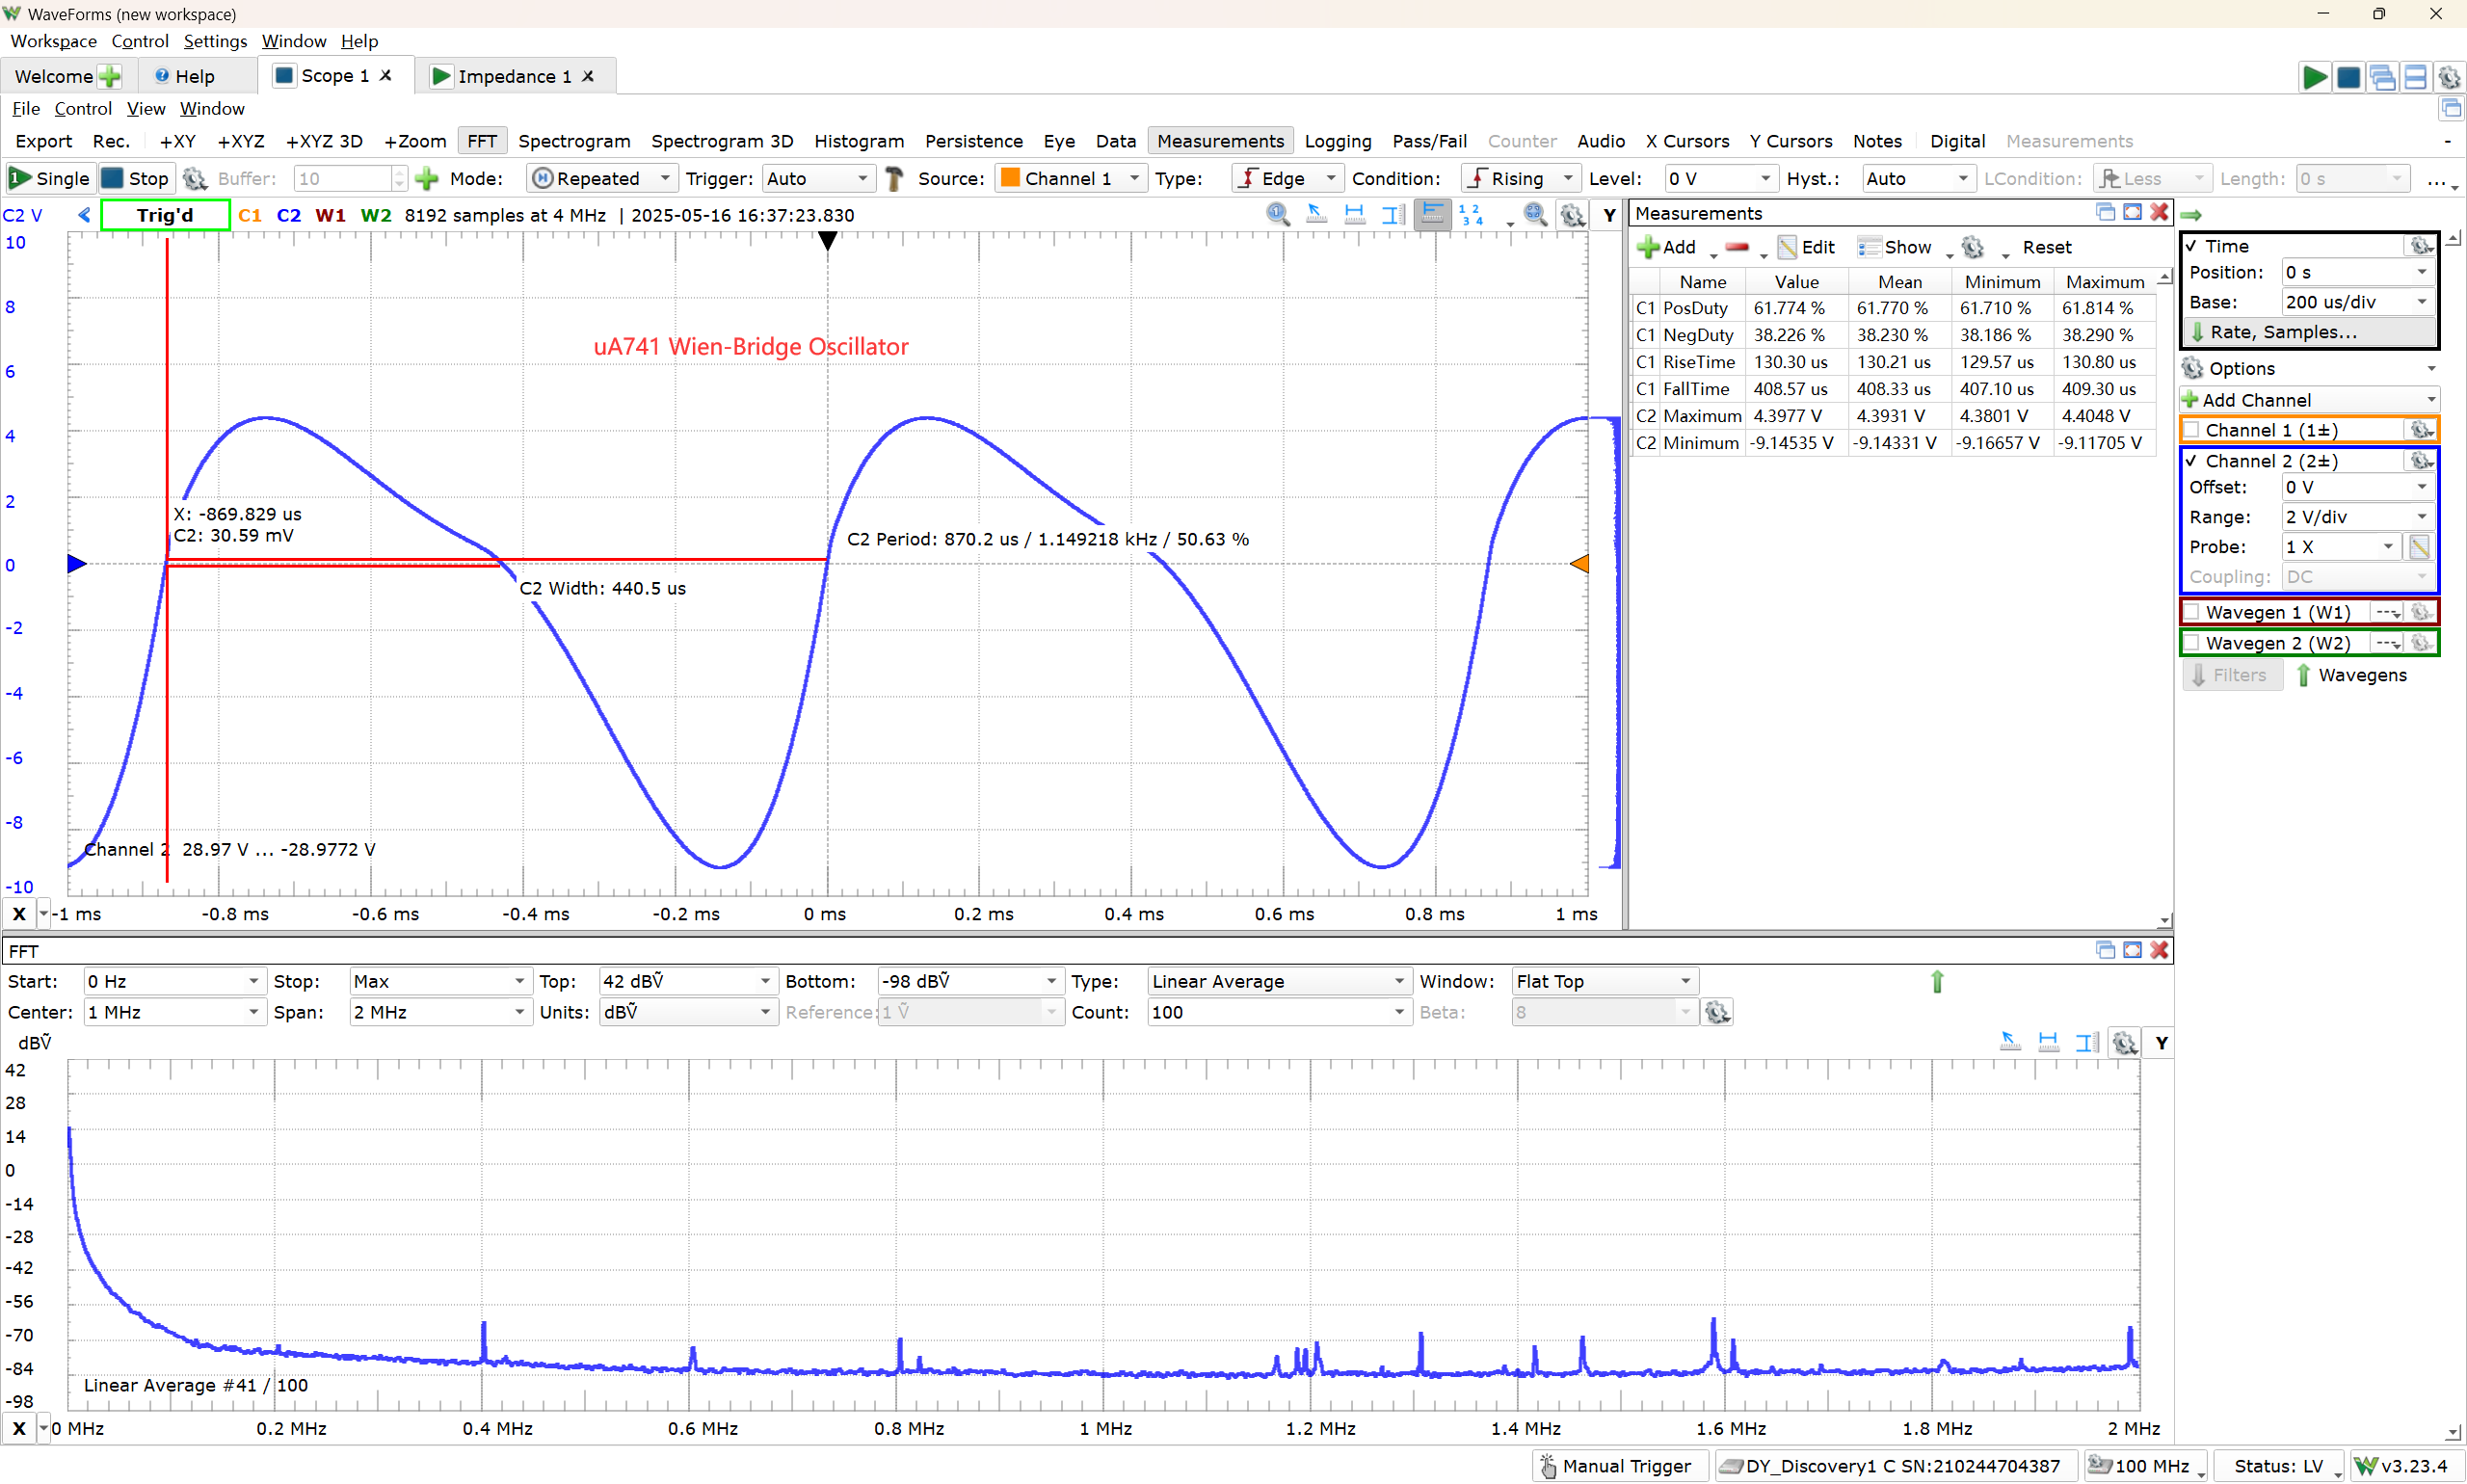
\includegraphics[width=\columnwidth]{LCE-06-07-运放设计/assets/uA741/test/wien 1.png}
    \caption{uA741 Wien-bridge oscillator: CH2 (blue) output}
\end{figure}

\begin{figure}[H]\centering
    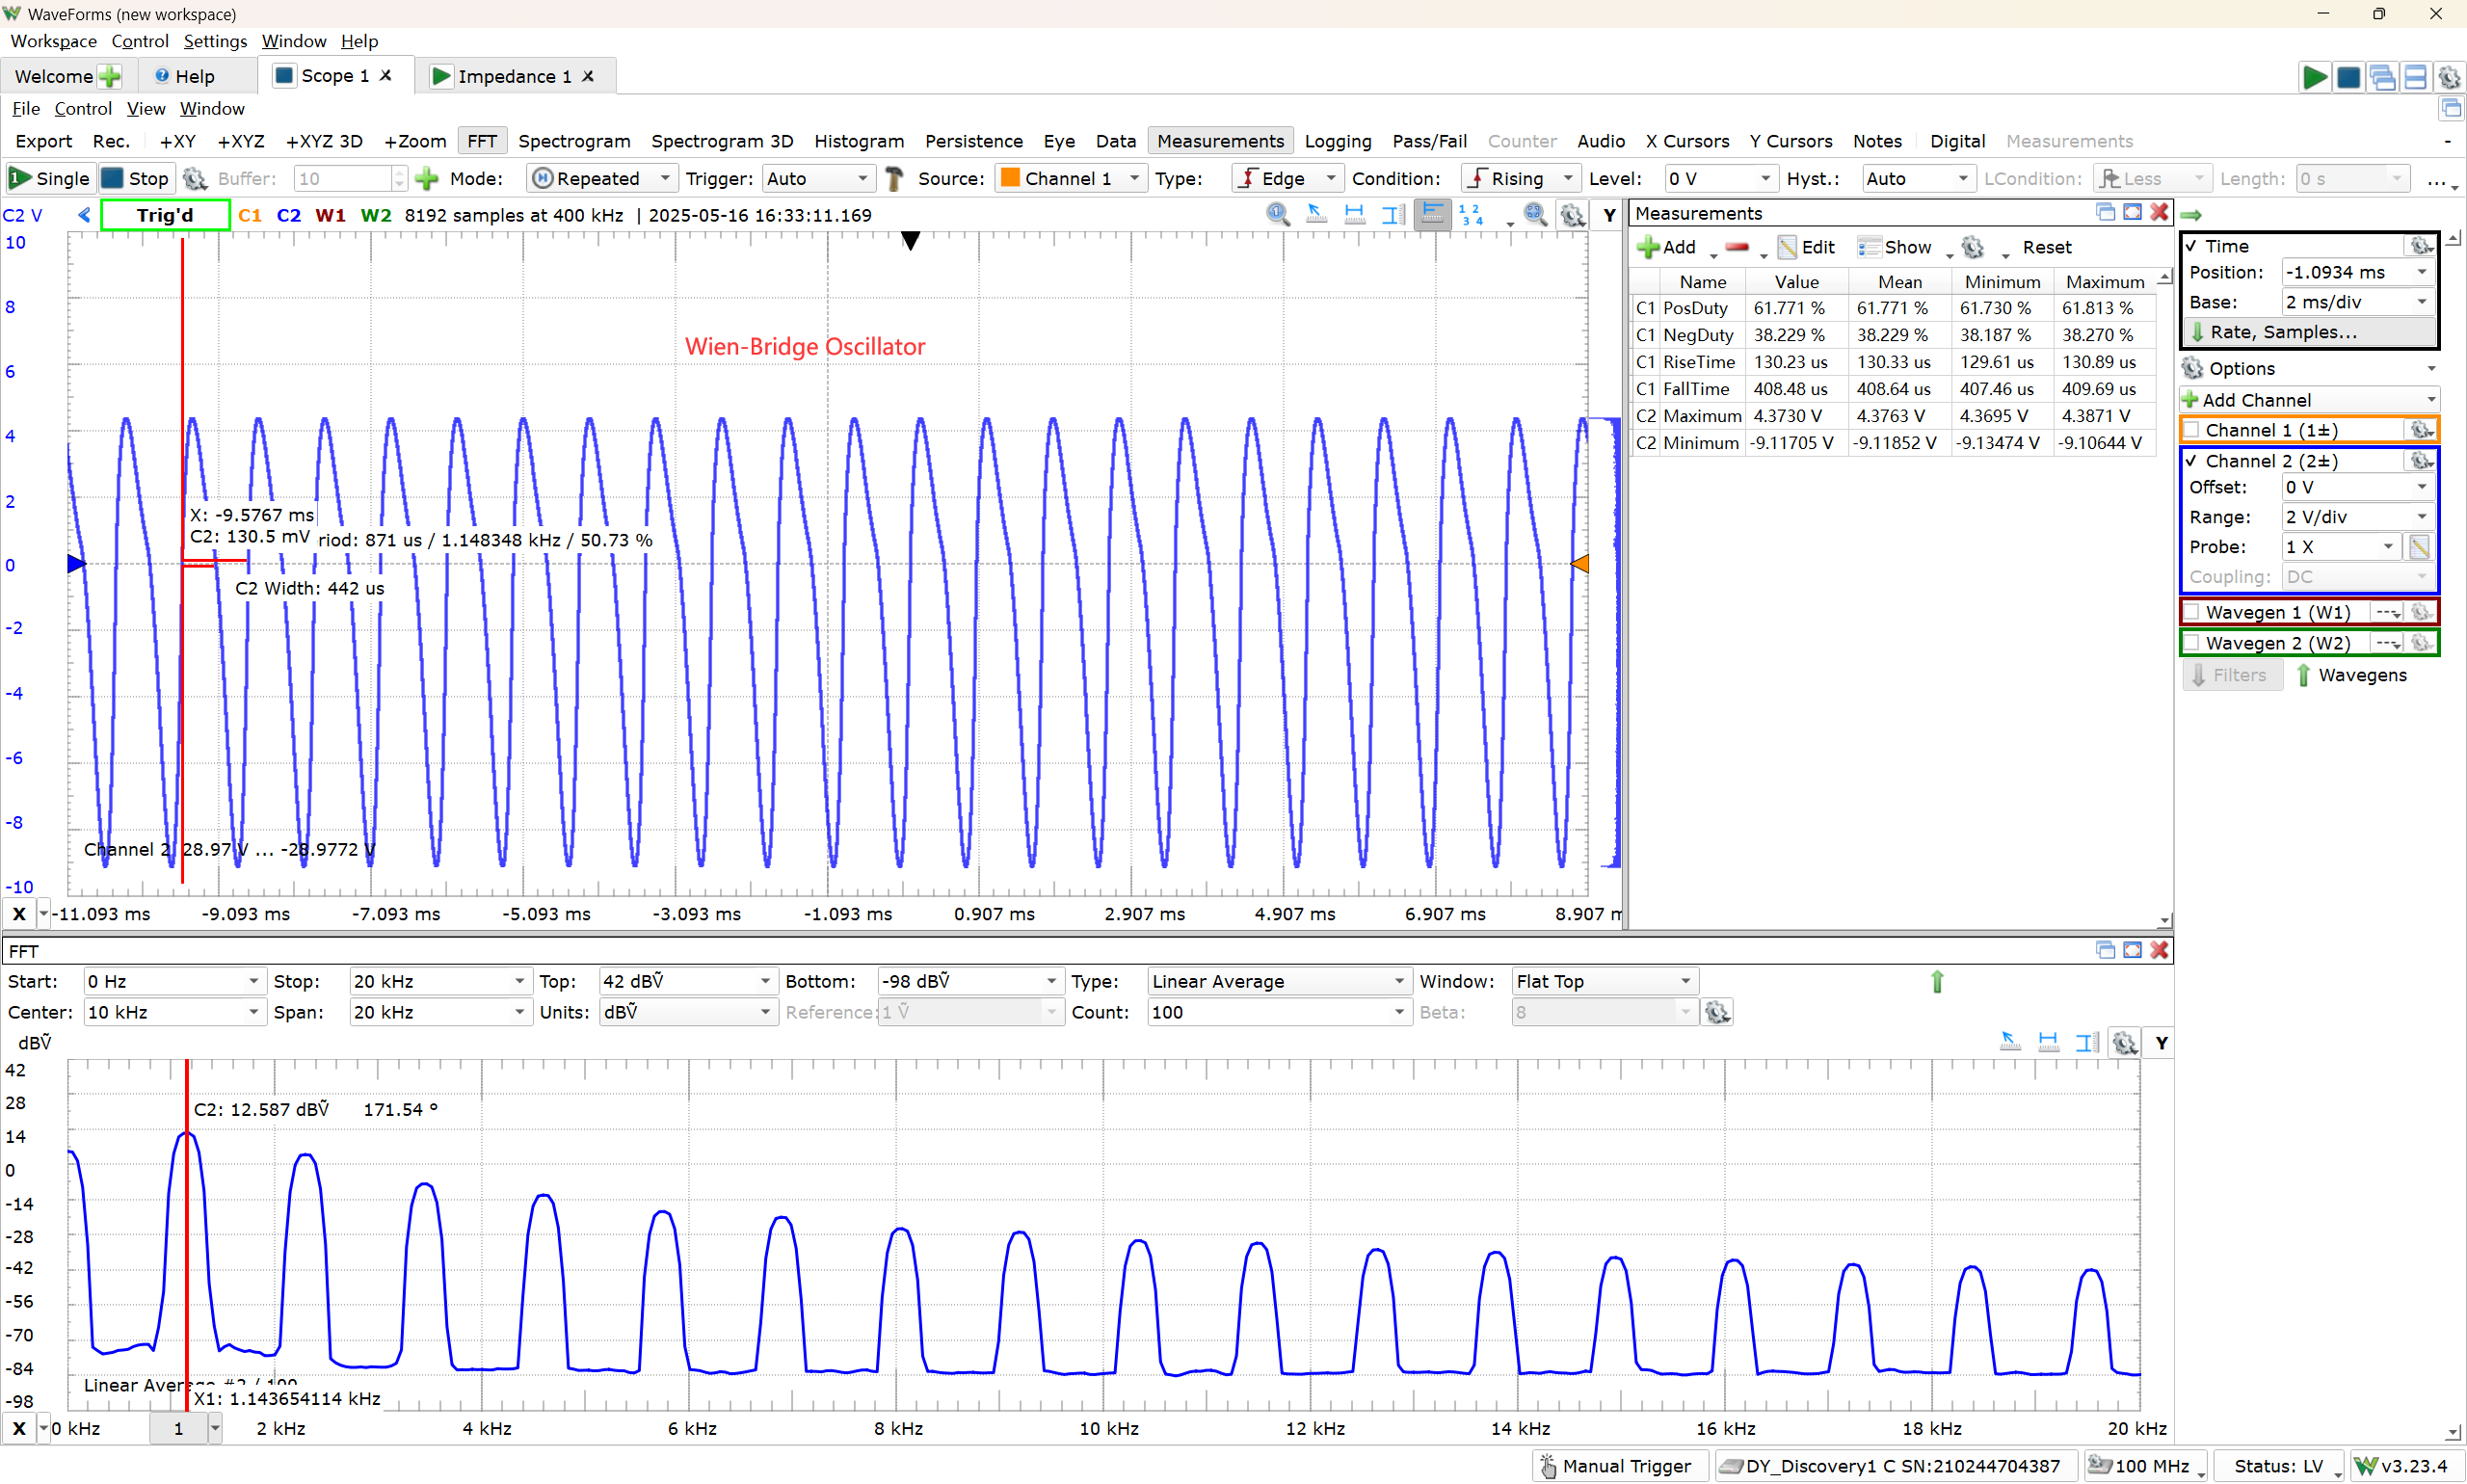
\includegraphics[width=\columnwidth]{LCE-06-07-运放设计/assets/uA741/test/wien 2.png}
    \caption{uA741 Wien-bridge oscillator: CH2 (blue) output; FFT results}
\end{figure}

\subsubsection{Op Amp Measurement of the Discrete μA741}

Use % 这里是链接
\href{https://yidingg.github.io/YiDingg/\#/ElectronicDesigns/Basic\%20Op\%20Amp\%20Measurement\%20Board\%20v2
}{ % 这里是文字
Basic Op Amp Measurement Board v2
} to measure the basic parameters of the discrete μA741, such as $V_{OS}\ I_{B\pm},\ A_{v,DC},\ \mathrm{PSRR}_{DC}$ and so on.
See % 这里是链接
\href{https://yidingg.github.io/YiDingg/#/Electronics/Op\%20Amp\%20Measurement\%20of\%20Discrete\%20uA741
}{ % 这里是文字
YiDingg's Website > Electronics Blogs > Op Amp Measurement of Discrete μA741
}
for the experiment record and the measurement results are shown below:


\begin{table}[H]\centering
    %\renewcommand{\arraystretch}{1.5} % 调整行间距
    %\setlength{\tabcolsep}{1.5mm} % 调整列间距
    \caption{Op Amp Measurement of the Discrete μA741}
    \label{Op Amp Measurement of the Discrete μA741}
\begin{tabular}{cccccccccc}\toprule
    Parameter & Symbol & Value \\
    \midrule
    Input offset voltage & $V_{OS}$ & + 3.5299 mV \\
    input bias current of inverting terminal & $I_{B-}$ & + 35.5542 nA \\
    input bias current of non-inverting terminal & $I_{B+}$ & + 41.8556 nA \\
    input bias current & $I_B$ & + 38.7049 nA \\
    input offset current & $I_{OS}$ & + 3.1507 nA \\
    DC open-loop gain & $A_{v,DC}$ & 79.822 dB \\
    AC open-loop gain @ 1 kHz & $A_{v,\mathrm{1kHz}}$ & 50.889 dB \\
    AC open-loop gain @ 10 kHz & $A_{v,\mathrm{10kHz}}$ & 29.143 dB \\
    AC open-loop gain @ 100 kHz & $A_{v,\mathrm{100kHz}}$ & 9.6738 dB \\
    DC power supply rejection ratio & $\mathrm{PSRR}_{DC}$ & 91.81 dB \\
    Gain Bandwidth product & $\mathrm{GBW}$ & 0.4090 MHz \\
    Phase margin & $\mathrm{PM}$ & 68.73° \\
    \bottomrule
\end{tabular}
\end{table}

\begin{figure}[H]\centering
    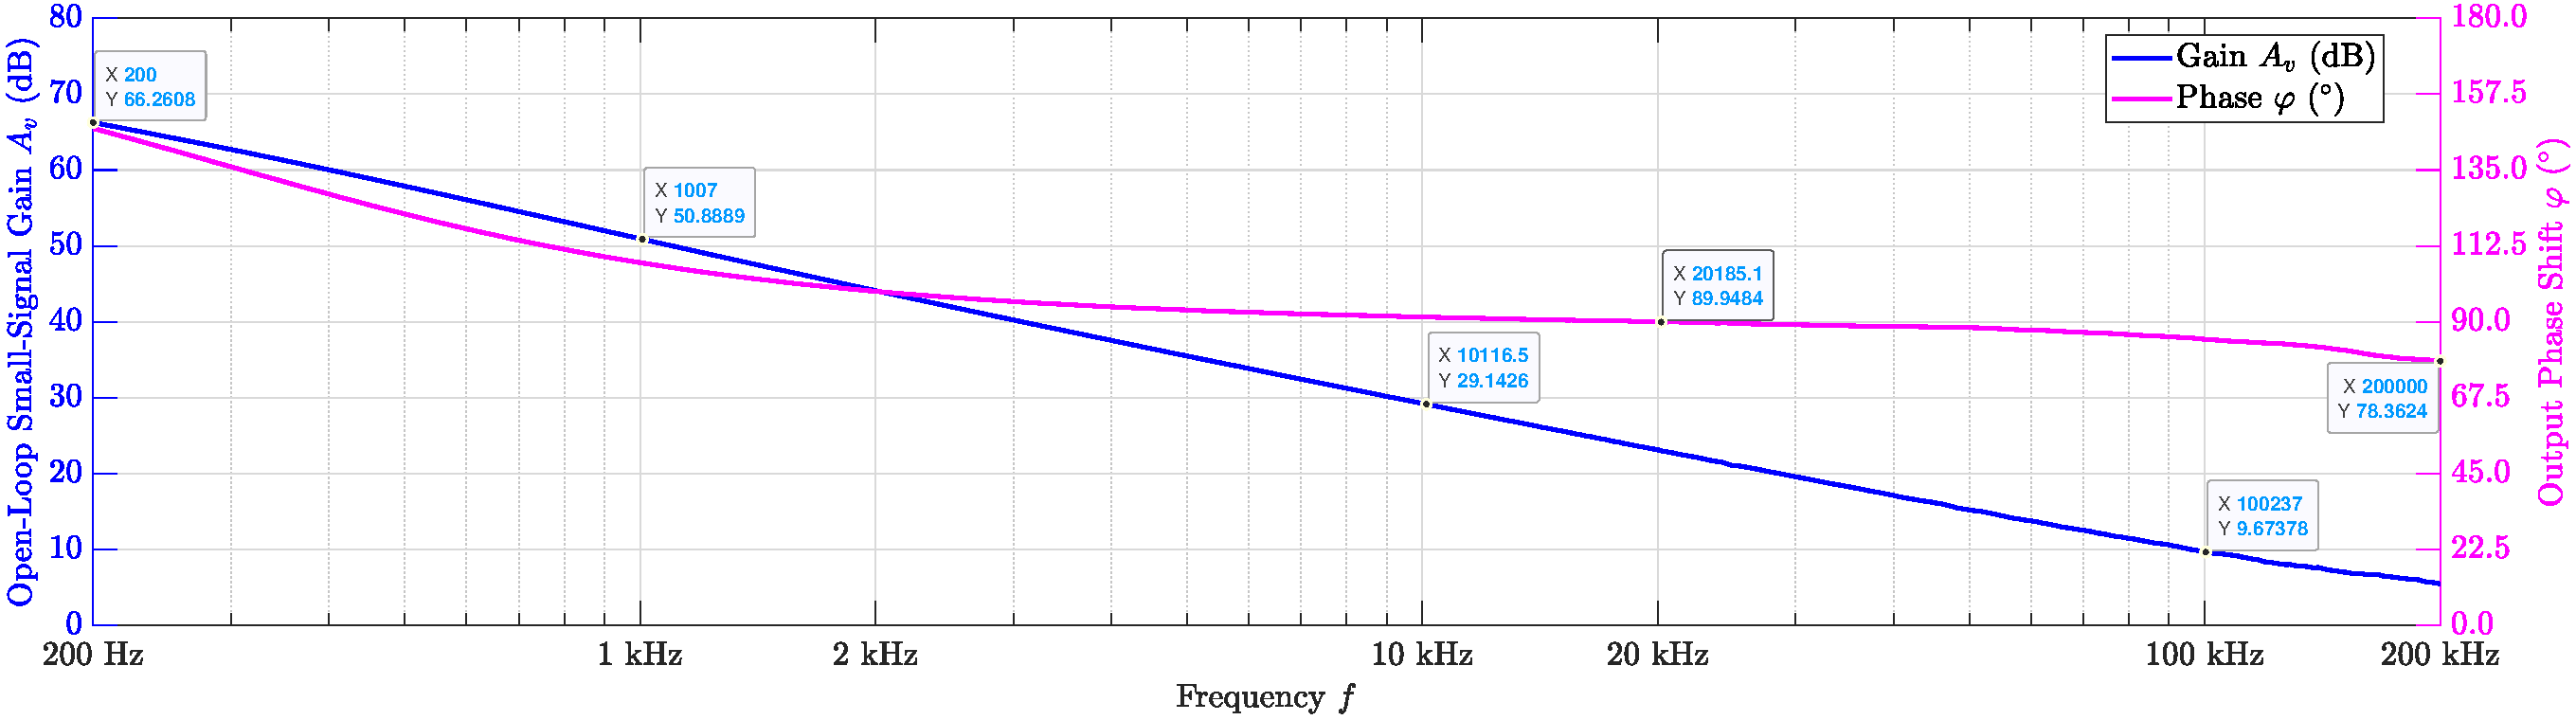
\includegraphics[width=\columnwidth]{LCE-06-07-运放设计/assets/uA741/test/2025-05-19_18-56-03.pdf}
    \caption{Frequency response of the discrete μA741}
\end{figure}

We can see that the dc voltage gain is obviously lower than the theoretical and simulated values (theoretical 155 V/mV, simulation 63 V/mV and experimental 9.8 V/mV). Possibly this error is due to the lower early voltage of the BJTs than that of the theoretical values. And, potentially, our DC gain measurement method might be somewhat inaccurate, causing the gain to be significantly underestimated. This point needs to be further verified.

\section{思考题}

\subsection{异常现象分析}

CMOS op amp 1 和 CMOS op amp 2 的实际补偿电容明显大于仿真值 (否则存在自激振荡)。举一个例子,在 CMOS op amp 2 的仿真中 (图 \ref{gain of CMOS op amp 2}),$C_c = 50\ \mathrm{pF}$ 便已经有约 $60^\circ$ 的相位裕度。但在 op amp 2 的实际测试结果中,即使是 $C_c = 100 \ \mathrm{pF}$ 也存在明显的自激振荡。为避免是 LTspice 中仿真模型的问题,我们在原先电路的基础上,按照数据手册上的典型值,手动添加了寄生电容 $C_{GS}$ 和 $C_{GD}$,此时的仿真结果如下:

\begin{figure}[H]\centering
    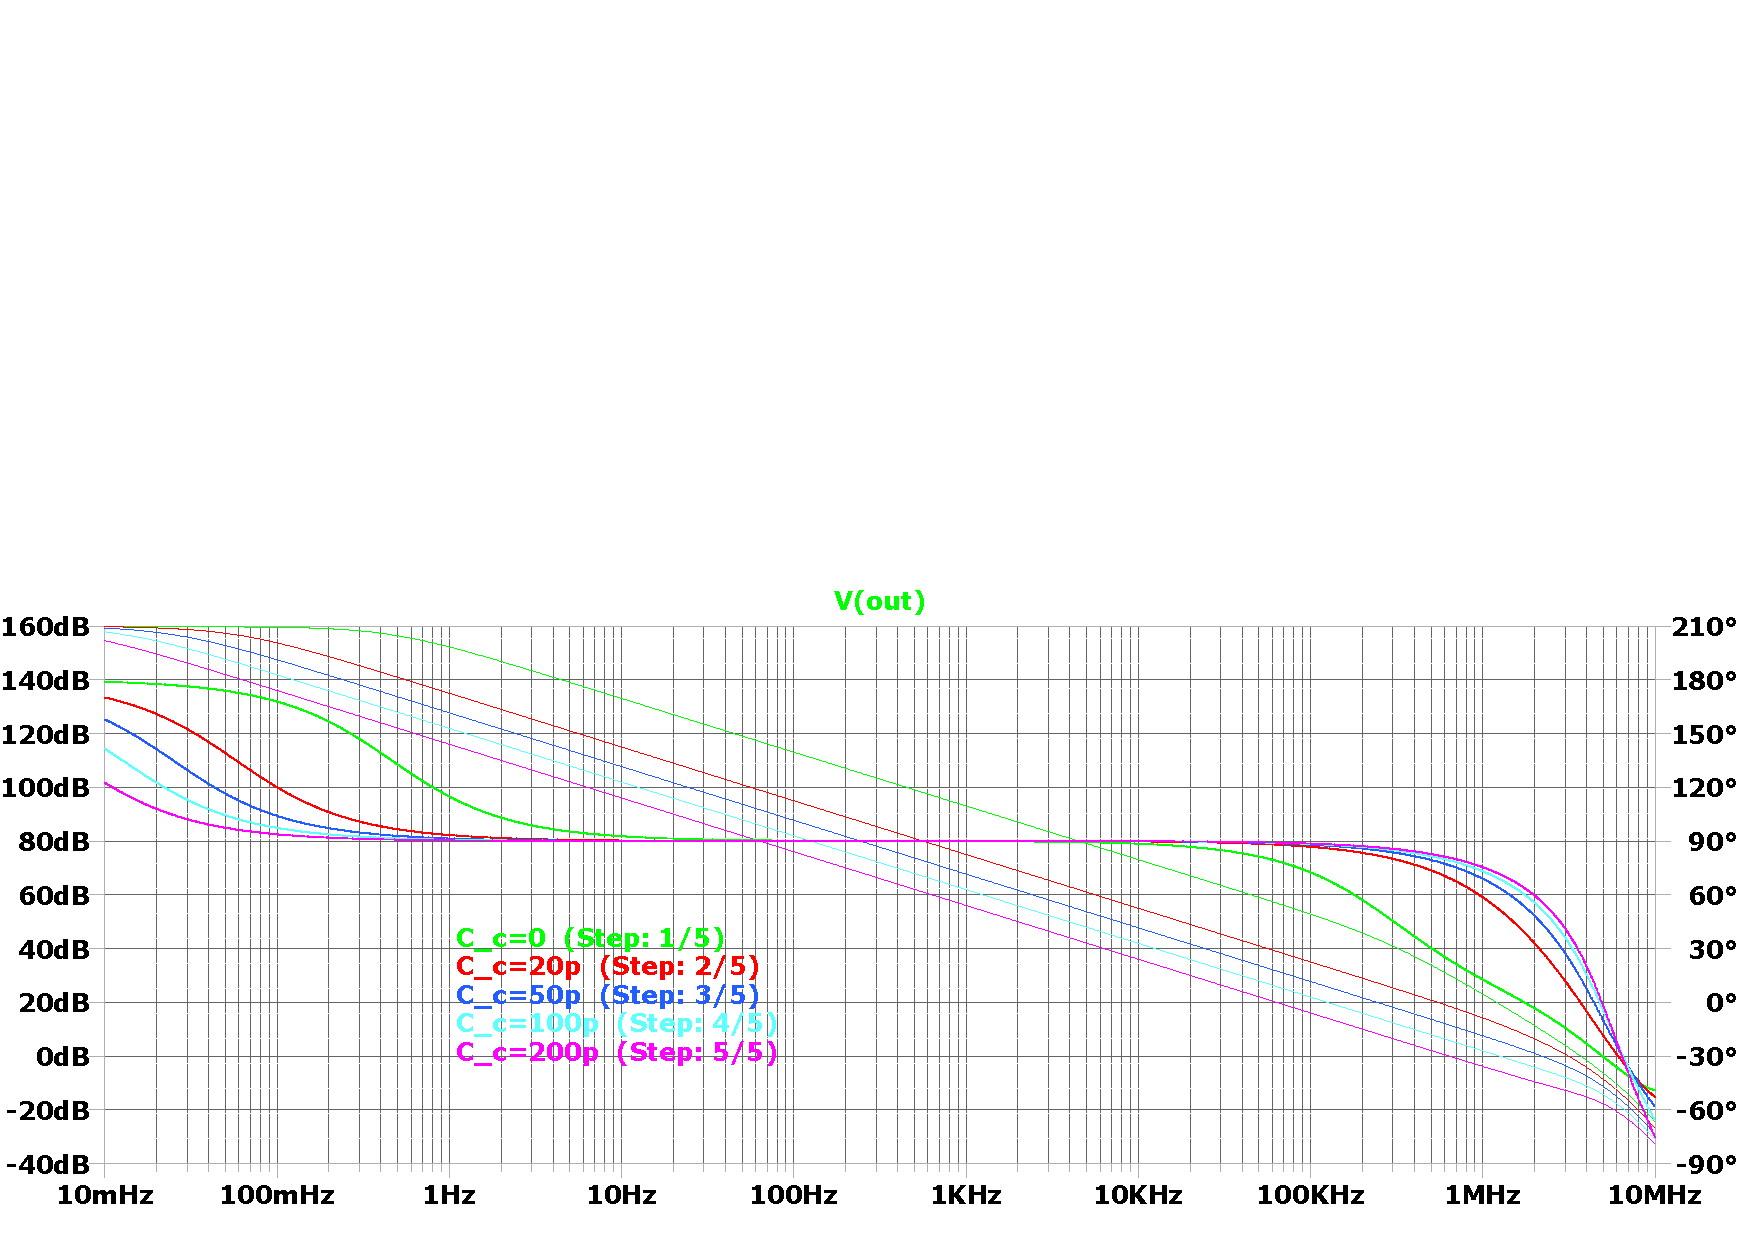
\includegraphics[width=\columnwidth]{LCE-06-07-运放设计/assets/appendix/gain of CMOS op amp 2 (with stray cap).pdf}
    \caption{Simulated frequency response of the CMOS op amp 2 with additional stray capacitances}
    \label{gain of CMOS op amp 2 (with stray cap)}
\end{figure}

图中可以看出,加了电容之后,$C_c = 50 \ \mathrm{pF}$ 的相位裕度降低到约 $43^\circ$,$C_c = 100 \ \mathrm{pF}$ 的相位裕度为 $68.5^\circ$,这仍然比实际测试时的补偿电容要小。实际补偿电容明显增大的具体原因,还有待进一步的讨论和探索。


\subsection{自主设计的分立运放,指标与通用运放 741 相比有无优点,为什么?}

优点:分立 uA741 具有更高的电源输入范围(因为分立元件耐压更高)和更高的最大输出电流,并且故障维修相对容易(更换元件即可)。缺点:器件参数更离散,电路匹配度降低使输入失调增大;并且,由于分立元件的寄生电容更大,运放的增益带宽积会减小,例如本次实验我们测得分立 uA741 的增益带宽积为 $0.4090 \ \mathrm{MHz}$,而 TI 集成 uA741 的增益带宽积为 $4.0 \ \mathrm{MHz}$ (typ.)。

缺点:静态功耗更高;器件参数离散,匹配度降低,失配更明显,导致输入失调增大 ($V_{OS}$ 和 $I_{OS}$)。

\subsection{运放的型号极为丰富,现实工作时是否会有自行设计运放的需求?}

排除某些特殊领域会有单独的分立运放设计需求,但在大多数情况下,使用现有的技术成熟的集成运放是性价比最高的选择,这样可以更加经济、快捷地获得稳定可靠的电路。因此在现实工作时,基本没有自行设计分立运放的需求。





% \subsection*{4.1 \ \ }
% \subsection*{4.2 \ \ }
% \subsection*{4.3 \ \ }
% \subsection*{4.4 \ \ }
% \subsection*{4.5 \ \ }
% \subsection*{4.6 \ \ }





















































\newpage
% 附录
\section*{附录 A\hspace*{20pt} 原始数据记录表}
\addcontentsline{toc}{section}{附录 A\hspace*{6pt} 原始数据记录表} 
\thispagestyle{fancy} 

\begin{enumerate}

\item Detailed explanations of the discrete uA741:
% 这里是链接
\href{https://yidingg.github.io/YiDingg/#/Electronics/Detailed\%20Explanation\%20of\%20uA741
}{ % 这里是文字
\\
YiDingg's Website > Electronics Blogs > Detailed Explanation of Classic Op Amp uA741\\
{\color{gray}\small https://yidingg.github.io/YiDingg/\#/Electronics/Detailed\%20Explanation\%20of\%20uA741}
}

\item Parameters measurement of the discrete μA741:
% 这里是链接
\href{https://yidingg.github.io/YiDingg/#/Electronics/Op\%20Amp\%20Measurement\%20of\%20Discrete\%20uA741
}{ % 这里是文字
\\
YiDingg's Website > Electronics Blogs > Op Amp Measurement of Discrete uA741\\
{\color{gray}\small https://yidingg.github.io/YiDingg/\#/Electronics/Op\%20Amp\%20Measurement\%20of\%20Discrete\%20uA741}
}

\item Parameters measurement of the discrete CMOS op amp 1 (CS):
% 这里是链接
\href{https://yidingg.github.io/YiDingg/#/Electronics/Op\%20Amp\%20Measurement\%20of\%20Discrete\%20CMOS\%20Op\%20Amp\%201\%20(CS)
}{ % 这里是文字
\\
YiDingg's Website > Electronics Blogs > Op Amp Measurement of Discrete CMOS Op Amp 1 (CS)\\
{\color{gray}\footnotesize https://yidingg.github.io/YiDingg/\#/Electronics/Op\%20Amp\%20Measurement\%20of\%20Discrete\%20CMOS\%20Op\%20Amp\%201\%20(CS)}
}

\item Parameters measurement of the discrete CMOS op amp 2 (PP):
% 这里是链接
\href{https://yidingg.github.io/YiDingg/#/Electronics/Op\%20Amp\%20Measurement\%20of\%20Discrete\%20CMOS\%20Op\%20Amp\%202\%20(PP)
}{ % 这里是文字
\\
YiDingg's Website > Electronics Blogs > Op Amp Measurement of Discrete CMOS Op Amp 2 (PP)\\
{\color{gray}\footnotesize https://yidingg.github.io/YiDingg/\#/Electronics/Op\%20Amp\%20Measurement\%20of\%20Discrete\%20CMOS\%20Op\%20Amp\%202\%20(PP)}
}

\item PCB design of the CMOS op amps:
% 这里是链接
\href{https://yidingg.github.io/YiDingg/#/ElectronicDesigns/Basic\%20CMOS\%20Op\%20Amp\%20using\%20Discrete\%20MOSFETs
}{ % 这里是文字
\\
YiDingg's Website > Electronic Designs > Basic CMOS Op Amp using Discrete MOSFETs\\
{\color{gray}\small https://yidingg.github.io/YiDingg/\#/ElectronicDesigns/Basic\%20CMOS\%20Op\%20Amp\%20using\%20Discrete\%20MOSFETs}
}\vspace*{-5mm}
\item PCB design of the discrete  μA741:
% 这里是链接
\href{https://yidingg.github.io/YiDingg/#/ElectronicDesigns/\%CE\%BCA741\%20using\%20Discrete\%20BJTs\%20(SOT-23)
}{ % 这里是文字
\\
YiDingg's Website > Electronic Designs > μA741 (Op Amp) using Discrete BJTs (SOT-23)\\
{\color{gray}\small https://yidingg.github.io/YiDingg/\#/ElectronicDesigns/\%CE\%BCA741\%20using\%20Discrete\%20BJTs\%20(SOT-23)}
}


\end{enumerate}


% 附录
\section*{附录 B \hspace*{20pt} Matlab Codes}
\addcontentsline{toc}{section}{附录 B \hspace*{6pt} Matlab Codes} 
\thispagestyle{fancy} 
\lstinputlisting{D:/a_RemoteRepo/GH.MatlabCodes/本科课程代码/Linear Circuit Experiment/LCE_06_07.m}



\newpage
% 附录
\newpage
\vspace*{\fill}\begin{center}\Huge{\bfseries 
    附录 C\hspace*{20pt} 实验预习报告
}\end{center}\addcontentsline{toc}{section}{附录 C\hspace*{6pt} 实验预习报告} 
\vfill
\thispagestyle{fancy} 
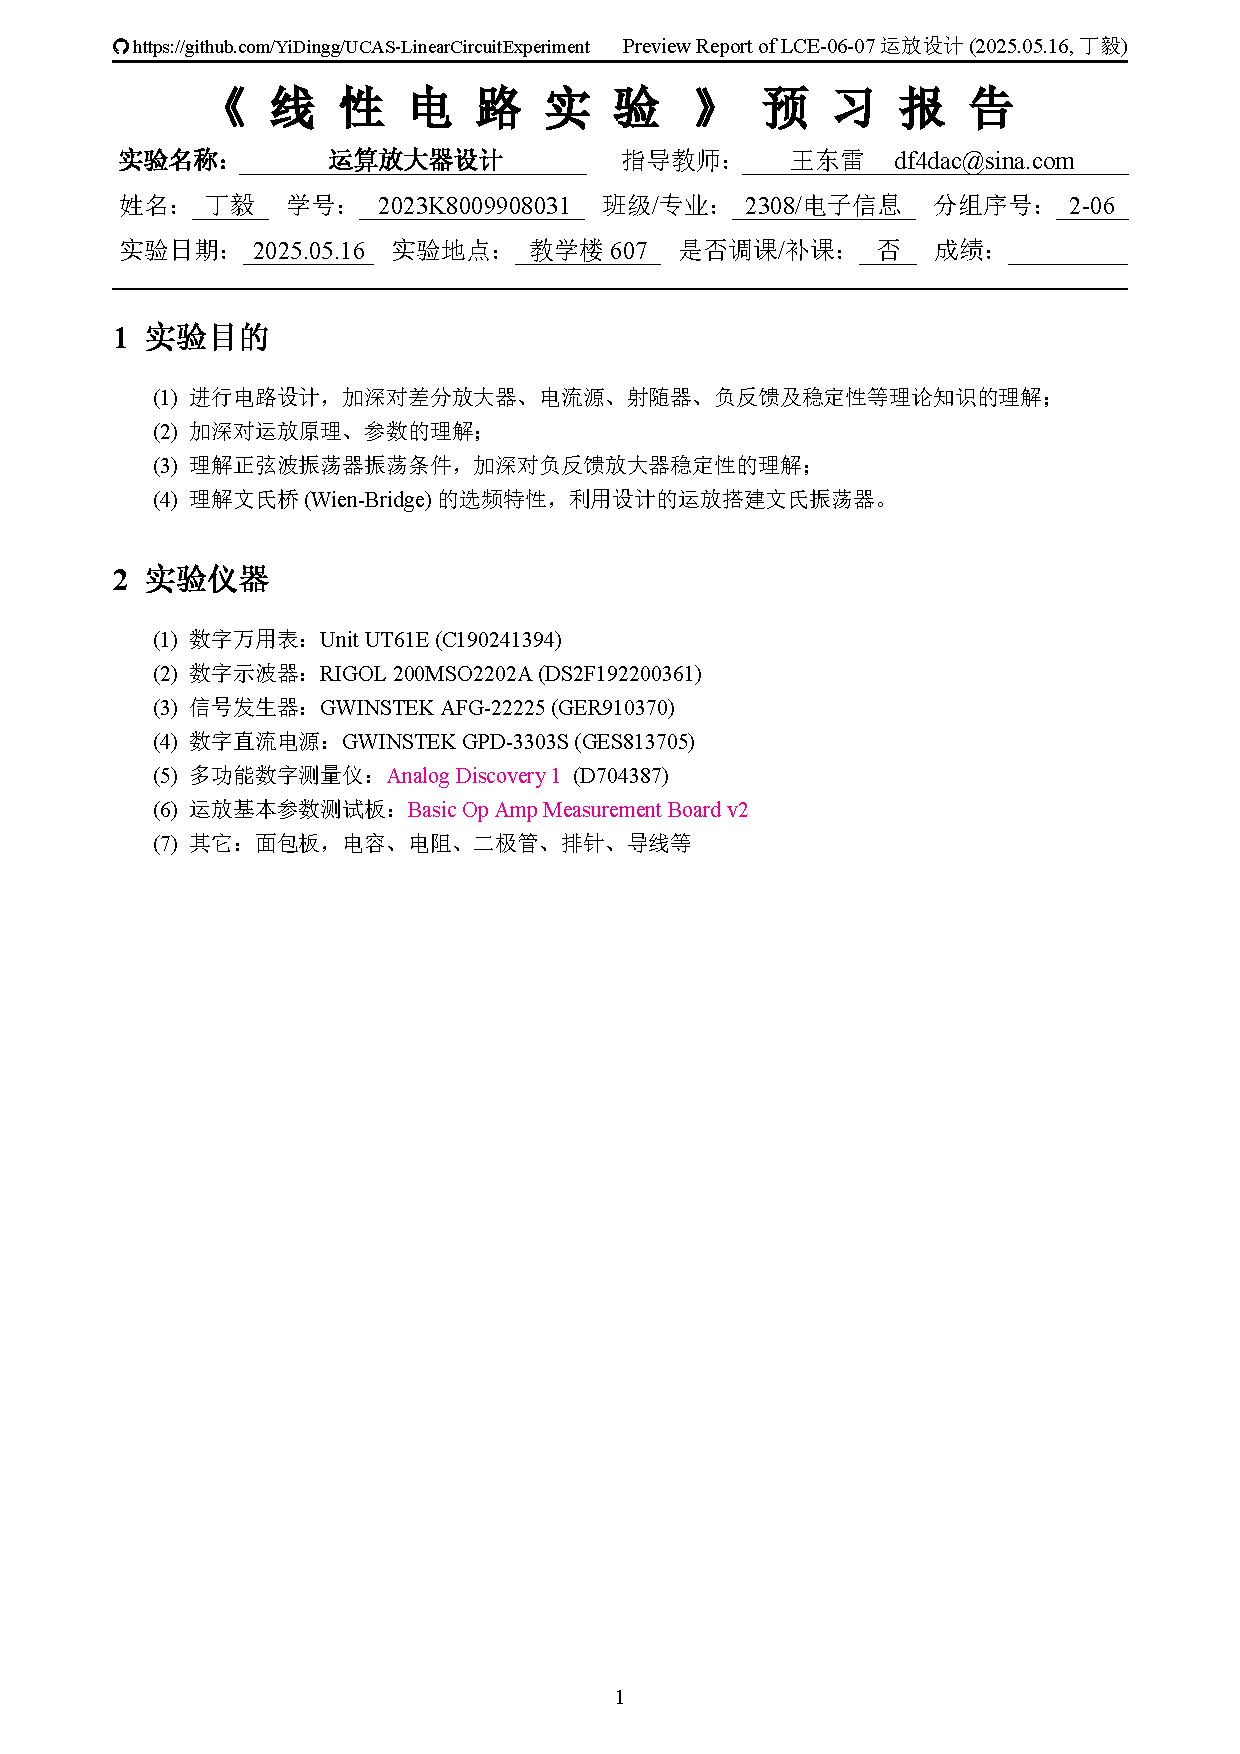
\includepdf[pages={-}]{LCE-06-07-运放设计/preview/LCE-06-07 (preview report).pdf}




















\end{document}

% VScode 常用快捷键:

% F2:                       变量重命名
% Ctrl + Enter:             行中换行
% Alt + up/down:            上下移行
% 鼠标中键 + 移动:           快速多光标
% Shift + Alt + up/down:    上下复制
% Ctrl + left/right:        左右跳单词
% Ctrl + Backspace/Delete:  左右删单词    
% Shift + Delete:           删除此行
% Ctrl + J:                 打开 VScode 下栏(输出栏)
% Ctrl + B:                 打开 VScode 左栏(目录栏)
% Ctrl + `:                 打开 VScode 终端栏
% Ctrl + 0:                 定位文件
% Ctrl + Tab:               切换已打开的文件(切标签)
% Ctrl + Shift + P:         打开全局命令(设置)

% Latex 常用快捷键:

% Ctrl + Alt + J:           由代码定位到PDF


